\documentclass[12pt,italian]{article}
\usepackage[T1]{fontenc}
\usepackage{babel}
\usepackage[utf8]{inputenc}
\usepackage{enumitem}
\usepackage{subfiles}
\usepackage{multirow}
\usepackage{color}
\usepackage{titlesec}
\usepackage{longtable}
\usepackage{xcolor,colortbl}
\usepackage[hidelinks]{hyperref}
\usepackage{graphicx}
\usepackage{adjustbox}
\usepackage{amsmath}
\usepackage{mdframed}
\usepackage{listings}
\usepackage{minted}
\usepackage{subfigure}
\usepackage{changepage}

\usepackage[a4paper,right=25mm,top=25mm,bottom=25mm, left=25mm]{geometry}
\usepackage{afterpage}
\usepackage{array,ragged2e}
\usepackage{booktabs}

\titlespacing*{\section}
{0pt}{20pt}{30pt}

\titlespacing*{\subsection}
{0pt}{20pt}{30pt}

\titlespacing*{\subsubsection}
{0pt}{20pt}{25pt}

\setlist[itemize]{noitemsep, topsep=0pt}



\graphicspath{
  {./immagini/}
}

\definecolor{LightGray}{gray}{0.9}

\definecolor{codegreen}{rgb}{0,0.6,0}
\definecolor{codegray}{rgb}{0.5,0.5,0.5}
\definecolor{codepurple}{rgb}{0.58,0,0.82}
\definecolor{backcolour}{rgb}{0.95,0.95,0.92}

\newcolumntype{P}[1]{>{\RaggedRight\arraybackslash}p{#1}}
\renewcommand{\baselinestretch}{1.5} 

\newlist{tabitem}{itemize}{1}
\setlist[tabitem]{nosep,
                  topsep     = 0pt,
                  partopsep  = 0pt,
                  leftmargin = *,
                  label      = \textbullet,
                  before = \vspace{-1\baselineskip},
                  after = \vspace{-0.5\baselineskip}}

\hypersetup{
    linktoc=all,
    pdfpagemode=FullScreen,
}
\definecolor{Gray}{gray}{0.85}
\definecolor{LightCyan}{rgb}{0.88,1,1}


\newcommand{\mycomment}[1]{}

\mycomment{}

\begin{document}


\begin{titlepage}
    
\pagestyle{empty}
\newgeometry{
    left=20mm,
    right=20mm,
    top=20mm,
    bottom=20mm
}


\begin{center}

% marchio di ateneo

\includegraphics[width=6.5cm,height=4.7cm]{marchio-di-ateneo_gs.png}

\vspace{10mm}

% \large is 12pt
{\normalsize{\bf{DIPARTIMENTO DI INFORMATICA - SCIENZA e INGEGNERIA}}} 

\vspace{5mm}

{\large{\bf{CORSO DI LAUREA MAGISTRALE IN INGEGNERIA INFORMATICA}}}

\vspace{23mm}

{\LARGE{\bf Analisi, Progettazione e Distribuzione in Cloud di applicativo multipiattaforma}}\\
\vspace{3mm}
{\LARGE{\bf per l'organizzazione di eventi condivisi e la condivisione multimediale automatica in tempo reale}}\\
\vspace{3mm}
%{\Huge{\bf }}\\
\vspace{3mm}

\end{center}

\vspace{32mm}

\begin{minipage}[t]{0.40\textwidth}
{\Large{\bf Relatore: \\ Chiar.mo Prof.\\ Michele Colajanni}}

\vspace{3mm}

{\Large{\bf }}
\end{minipage}
\hfill
\begin{minipage}[t]{0.40\textwidth}\raggedleft
{\Large{\bf Presentata da: \\ Giacomo Romanini}}
\end{minipage}

\vspace{10mm}

\rule[0.5cm]{15.8cm}{0.6mm}

\begin{center}
{\large{\bf Sessione Marzo 2025 \\}}
{\large{\bf Anno Accademico 2024/2025\\}}
\end{center}

\end{titlepage}

\restoregeometry



\section*{Abstract}


Lo sviluppo di un applicativo multipiattaforma diretto all’organizzazione di eventi condivisi, 
caratterizzato in particolare dalla condivisione multimediale in tempo reale, richiede opportune capacità di scalabilità, 
atte a garantire una risposta efficace anche con alti volumi di richieste, offrendo prestazioni ottimali. 
Le tecnologie cloud, con la loro disponibilità pressoché illimitata di risorse e alla completa e continua garanzia  di manutenzione, 
offrono l'architettura ideale per il supporto di simili progetti. \\
Tuttavia, l'integrazione tra la logica applicativa ed i molteplici servizi cloud, insieme alla gestione delle loro interazioni reciproche, 
comporta sfide specifiche, in particolare legate all'ottimizzazione di tutte le risorse. 
L’individuazione e la selezione delle soluzioni tecnologiche più adatte per ogni obiettivo
e l'adozione delle migliori pratiche progettuali devono procedere parallelamente con lo sviluppo del codice, al fine di sfruttare efficacemente le potenzialità offerte. \\
In tale prospettiva, questa tesi illustra le scelte progettuali e implementative adottate nello sviluppo dell'applicativo in questione, 
evidenziando l’impatto dell'integrazione delle risorse cloud sul risultato finale.
\clearpage
\pagenumbering{gobble}
\tableofcontents
\clearpage
\pagenumbering{arabic}
%

\section*{Introduzione}
\addcontentsline{toc}{section}{Introduzione}


In un contesto sempre più connesso, la crescente quantità di contatti, la rapidità delle comunicazioni e l'accesso universale alle informazioni rendono la creazione, l'organizzazione e la partecipazione ad eventi estremamente facile, ma al contempo generano un ambiente frenetico e spesso dispersivo.\\
Risulta infatti difficile seguire tutte le opportunità a cui si potrebbe partecipare, considerando le numerose occasioni che si presentano quotidianamente, rischiando di ricordarsene solo successivamente, una volta passate. Basti pensare, ad esempio, alle riunioni di lavoro, alle serate con amici, agli appuntamenti informali per un caffè, ma anche a eventi più strutturati come fiere, convention aziendali, concerti, partite sportive o mostre di artisti che visitano occasionalmente la città.\\
Questi eventi possono sovrapporsi, causando dimenticanze o conflitti di pianificazione, con il rischio di delusione o frustrazione. Quando si è invitati a un evento, può capitare di essere già impegnati, o di trovarsi in attesa di una conferma da parte di altri contatti. In questi casi, la gestione degli impegni diventa complessa: spesso si conferma la partecipazione senza considerare possibili sovrapposizioni, o dimenticandosi, per poi dover scegliere e disdire all'ultimo momento. \\
D’altra parte, anche quando si desidera proporre un evento, la ricerca di un'attività interessante può diventare un compito arduo, con la necessità di consultare numerosi profili social di locali e attività, senza avere inoltre la certezza che gli altri siano disponibili.\\
Tali problemi si acuiscono ulteriormente quando si tratta di organizzare eventi di gruppo, dove bisogna allineare gli impegni di più persone. \\
In questo contesto, emergono la necessità e l'opportunità di sviluppare uno strumento che semplifichi la proposta e la gestione degli eventi, separando il momento della proposta da quello della conferma di partecipazione. In tal modo, gli utenti possono valutare la disponibilità degli altri prima di impegnarsi definitivamente, facilitando l'invito e la partecipazione.\\ 
\clearpage
In risposta a tali richieste è nata Wyd, un'applicazione che permette ai clienti di organizzare i propri impegni, siano essi confermati oppure proposti. Essa permette anche di rendere più intuitiva la ricerca di eventi attraverso la creazione di uno spazio virtuale centralizzato dove gli utenti possano pubblicare e consultare tutti gli eventi disponibili, diminuendo l’eventualità di perderne qualcuno. 
La funzionalità chiave di questo progetto si fonda sull'idea di affiancare alla tradizionale agenda degli impegni certi un calendario separato, che mostri tutti gli eventi a cui si potrebbe partecipare. Una volta confermata la partecipazione a un evento, questo verrà spostato automaticamente nell'agenda personale dell'utente.
Gli eventi creati potranno essere condivisi con persone o gruppi, permettendo di visualizzare le conferme di partecipazione. 
Inoltre, considerando l'importanza della condivisione di contenuti multimediali, questo progetto prevede la possibilità di condividere foto e video con tutti i partecipanti all'evento, attraverso la generazione di link per applicazioni esterne o grazie all'ausilio di gruppi di profili. Al termine dell’evento,
l'applicazione carica automaticamente le foto scattate durante l'evento,
per allegarle a seguito della conferma dell'utente.\\
\\
Come anticipato, la realizzazione di un progetto come Wyd implica la risoluzione e la gestione di diverse problematiche tecniche. 
In primo luogo, garantire la persistenza dell'agenda dell'utente, che deve essere aggiornata e mantenuta in modo affidabile e coerente, tale da permettere per un uso distribuito del servizio. 
Inoltre, la funzionalità di condivisione degli eventi richiede l'aggiornamento in tempo reale di tutti gli utenti coinvolti, al fine di rimanere sempre aggiornati. 
Infine, il caricamento e il salvataggio delle foto introduce la necessità di gestire richieste di archiviazione di dimensioni significative.
In questa prospettiva, risulta fondamentale esplorare il procedimento di analisi e progettazione che ha portato allo sviluppo di un applicativo multipiattaforma efficace, affidabile e scalabile, in grado di soddisfare le esigenze degli utenti nell’ambito dell'organizzazione di eventi condivisi e della condivisione multimediale automatica in tempo reale.
Seguendo l’esame dei requisiti necessari, l’analisi dello sviluppo del progetto affronterà in una prima parte le scelte infrastrutturali che hanno portato a definire la struttura centrale dell’applicazione, spiegando brevemente i requisiti e le soluzioni trovate. 
Successivamente si osserverà lo studio effettuato per gestire la memoria, in quanto fattore che più incide sulle prestazioni. Particolare attenzione è stata dedicata, infatti, a determinare le tecnologie e i metodi che meglio corrispondono alle esigenze derivate dal salvataggio e dall’interazione logica degli elementi.
Infine, per permettere la gestione delle immagini, che introducono problematiche impattanti sia sulle dimensioni delle richieste sia sull'integrazione con la persistenza, una terza parte si concentrerà sulle scelte implementative adottate per l’inserimento delle funzionalità.


\clearpage

\section{L'Analisi delle funzionalità}

La realizzazione di qualunque prodotto software inizia da una fase in cui, 
partendo dall’abstract del progetto, si analizzano i requisiti e le funzionalità da realizzare.
L’obiettivo è arrivare ad una definizione delle proprietà e del comportamento desiderato nell’applicazione che sia concisa e condivisa col cliente,
senza però entrare nel merito delle scelte implementative.\\
Solo a quel punto si può procedere con la progettazione del programma vero e proprio.

\subsection{I requisiti e i casi d’uso}

Lo studio dell’abstract del progetto porta all’individuazione e alla descrizione delle sue caratteristiche essenziali.
In particolare, si distinguono i requisiti ed i casi d'uso.
I requisiti formalizzano le funzionalità che l'applicazione deve fornire, 
sintetizzando e schematizzando le parti che descrivono del prodotto.
I casi d'uso descrivono invece le interazioni previste tra l'utente e il sistema, 
suddividendo le funzionalità in azioni elementari.\\

\subsubsection{I requisiti e il vocabolario}
I requisiti devono risultare chiari e precisi per permettere di procedere alle fasi sucessive in maniera corretta e trasparente.
Ogni requisito deve essere breve e puntuale, limitato ad un solo particolare desiderata,
focalizzando una necessità specifica.\\
\\
Si suddividono in funzionali o non funzionali in base alle loro caratteristiche.\\
I requisiti funzionali descrivono le funzionalità che il sistema deve fornire,
mentre i requisiti non funzionali illustrano le caratteristiche che il sistema deve soddisfare per essere considerato valido.\\

Si noti come le caratteristiche di velocità e scalabilità vengono individuate ed introdotte fin da subito.
\begin{table}
    \begin{tabular} {|P{1.3cm}|P{11.2cm}|P{3cm}|}
        \hline
        \textbf{ID} & \textbf{Requisiti}                                                          & \textbf{Tipo}  \\
        \hline
        R1F         & Registrazione di un account tramite l’interfaccia web                       & Funzionale     \\
        \hline
        R2F         & Identificazione attraverso mail univoca e password di almeno 6 caratteri    & Funzionale     \\
        \hline
        R3F         & Visualizzazione degli eventi confermati                                     & Funzionale     \\
        \hline
        R4F         & Visualizzazione degli eventi proposti                                       & Funzionale     \\
        \hline
        R5F         & Creazione di un evento impostando almeno la data di inizio e quella di fine & Funzionale     \\
        \hline
        R6F         & La data di fine deve essere successiva alla data di inizio                  & Funzionale     \\
        \hline
        R7F         & Modifica di un evento                                                       & Funzionale     \\
        \hline
        R8F         & La conferma di un evento lo sposta negli eventi confermati                  & Funzionale     \\
        \hline
        R9F         & La disdetta di un evento lo sposta negli eventi proposti                    & Funzionale     \\
        \hline
        R10F        & Caricamento delle foto di un evento                                         & Funzionale     \\
        \hline
        R11F        & Condivisione tramite link                                                   & Funzionale     \\
        \hline
        R12F        & Condivisione tramite gruppo o ad altri profili                              & Funzionale     \\
        \hline
        R13F        & Ricerca automatica delle foto sul dispositivo mobile                        & Funzionale     \\
        \hline
        R14F        & Conferma delle foto                                                         & Funzionale     \\
        \hline
        R15F        & Ricerca di altri profili                                                    & Funzionale     \\
        \hline
        R16F        & Creazione di un gruppo da due o più profili                                 & Funzionale     \\
        \hline
        R17F        & Visualizzazione dei profili collegati                                       & Funzionale     \\
        \hline
        R18F        & Creazione di un nuovo profilo                                               & Funzionale     \\
        \hline
        R19F        & Cambio del profilo attualmente in uso                                       & Funzionale     \\
        \hline
        R20F        & Aggiornamento in tempo reale delle modifiche agli eventi                    & Funzionale     \\
        \hline
        R1NF        & Per interagire l’utente deve essere autenticato                             & Non Funzionale \\
        \hline
        R2NF        & Velocità di richiesta iniziale dei dati                                     & Non Funzionale \\
        \hline
        R3NF        & Semplicità e fluidità dell'interfaccia grafica                              & Non Funzionale \\
        \hline
        R4NF        & Velocità in lettura e scrittura dei dati                                    & Non Funzionale \\
        \hline
        R5NF        & Velocità nella ricerca dei profili                                          & Non Funzionale \\
        \hline
        R6NF        & Scalabilità delle richieste                                                 & Non Funzionale \\
        \hline
    \end{tabular}
    \caption{Tabella dei requisiti di Wyd}
\end{table}
\clearpage

Alla tabella dei requisiti si affianca quella del vocabolario, 
definendo i termini utilizzati nel progetto per allinearli definitivamente alle volontà del cliente.\\

\begin{table}[htb]
    \begin{tabular} {|P{3.5cm}|P{9cm}|P{3cm}|}
        \hline
        \textbf{Voce}     & \textbf{Definizione}                                                             & \textbf{Sinonimi}                 \\
        \hline
        Account           & combinazione di mail e password che identifica un utente                         &                                   \\
        \hline
        Utente            & Persona che utilizza l’applicazione                                              &                                   \\
        \hline
        Profilo           & Entità logica che raggruppa eventi e interazioni                                 &                                   \\
        \hline
        Profili collegati & Profili a cui l'utente può avere accesso                                         &                                   \\
        \hline
        Gruppo            & Insieme di profili                                                               &                                   \\
        \hline
        Evento            & Azione(o previsione di azione) con una durata nel tempo                          &                                   \\
        \hline
        Data e ora evento & Indicazione temporale del momento in cui avverrà l'azione                        &                                   \\
        \hline
        Evento confermato & Evento a cui il profilo ha dato conferma di partecipazione                       &                                   \\
        \hline
        Evento proposto   & Evento a cui il profilo non ha dato conferma di partecipazione                   & Evento disdetto, evento condiviso \\
        \hline
        Email             & Indirizzo di posta elettronica del cliente utilizzata anche per l'autenticazione &                                   \\
        \hline
        Password          & Codice alfanumerico di almeno 8 caratteri                                        &                                   \\
        \hline
        Credenziali       & Insieme composto da email e password necessari per accedere al sistema           &                                   \\
        \hline
    \end{tabular}
    \caption{Vocabolario di Wyd}
\end{table}

\clearpage


\subsubsection{I casi d’uso}

I casi d’uso descrivono le interazioni tra gli attori ed il sistema, suddividendo le funzionalità in azioni elementari.
Si definiscono attori tutti gli elementi che compiono una parte attiva nei confronti del programma.
Ogni attore può interagire con uno o più casi d'uso, 
ed ogni caso d'uso può essere relazionazionato con altri, definendo la loro relazione.\\
\\
I casi d'uso possono essere collegati tra loro tramite rapporti di inclusione o estensione.
Si dice che un caso include un altro se contiene il suo comportamento.
Si dice invece che un caso d'uso ne estende un altro se il suo comportamento può essere inserito all'interno del secondo.\\
\\

\begin{figure}[htb]
    \centering
    \adjustbox{width=\textwidth}{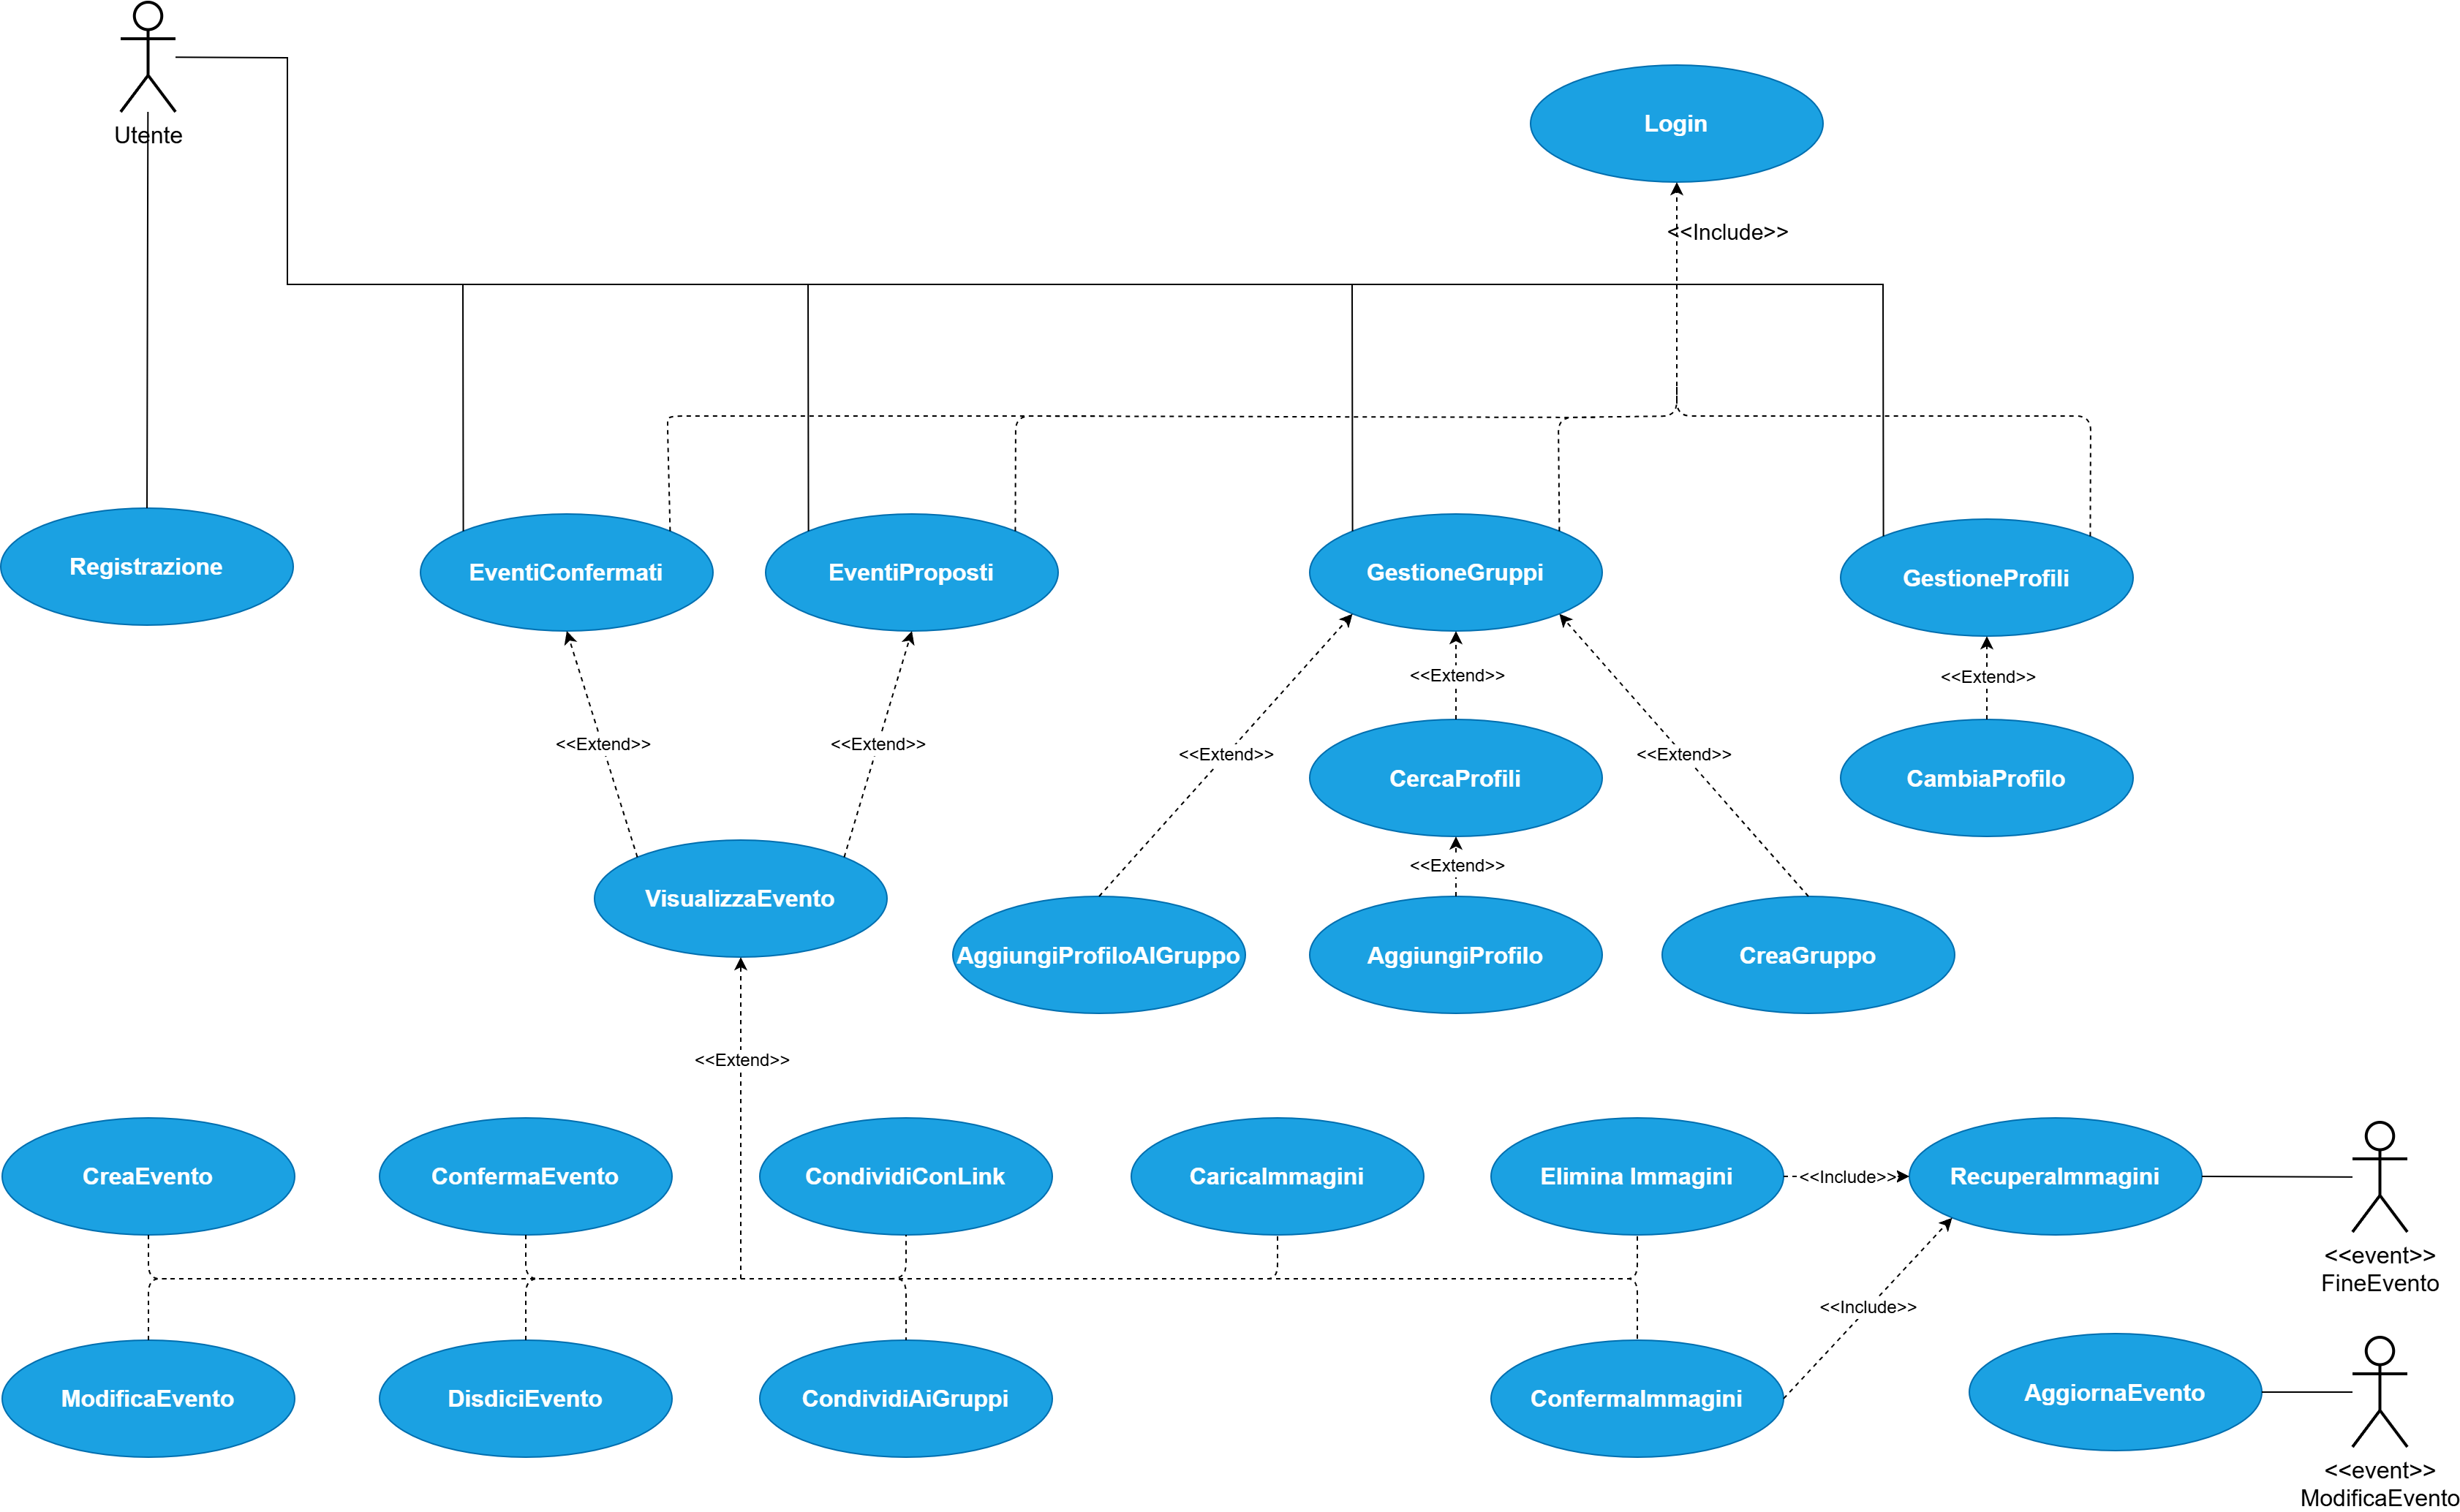
\includegraphics{Casiduso.png}}
    \caption{Diagramma dei casi d'uso}
\end{figure}
\clearpage
Per ogni caso d'uso viene identificato uno scenaro di utilizzo, che chiarifica il contesto, il comportamento ed i punti critici dell'utilizzo.
In particolare, si riportano gli scenari di utilizzo per i principali casi d'uso di Wyd, ovvero quelli
che più andranno ad impattare sulla struttura e sulle esigenze del progetto.\\
\\
Lo scenario di registrazione vede la responsabilità, oltre che di creare un account, di collegare un profilo all'utente.
Questa separazione consente di avere una struttura gerarchica che permette di associare più profili ad un'unico utente, che può così in seguito crearne o unirne di nuovi.\\

\begin{table}[htbp]
    \begin{tabular} {|P{4.5cm}|P{11cm}|}
        \hline
        \textbf{Titolo}                   & Registrazione                                                                         \\
        \hline
        \textbf{Descrizione}              & L'utente si registra al servizio                                                      \\
        \hline
        \textbf{Attori}                   & Utente                                                                                \\
        \hline
        \textbf{Relazioni}                &                                                                                       \\
        \hline
        \textbf{Precondizioni}            &                                                                                       \\
        \hline
        \textbf{Postcondizioni}           & L'utente è registrato nel sistema e può interagire con il resto dell'applicazione     \\
        \hline
        \textbf{Scenario principale}      & 1.L'utente accede alla schermata di registrazione      \newline
        2. L'utente inserisce email e  password                      \newline
        3. Il sistema crea un account con le credenziali inserite, associando un utente ed un primo profilo   \newline
        4. L'utente termina la registrazione, se avvenuta con successo viene reindirizzato alla pagina principale
        \\
        \hline
        \textbf{Scenari Alternativi}      &

        Il sistema verifica che è già presente un account con la mail inserita, quindi procede con la procedura di login normale. \\
        \hline
        \textbf{Requisiti non funzionali} &
        Per interagire l’utente deve essere autenticato \linebreak
        Velocità in lettura e scrittura dei dati                                                                                  \\
        \hline
        \textbf{Punti aperti}             &                                                                                       \\
        \hline
    \end{tabular}

    \caption{Scenario di registrazione}
\end{table}
\clearpage
A seguito della modifica di un evento, che implica il salvataggio dei suoi nuovi dati, viene chiesto l'aggiornamento in tempo reale verso tutte le parti interessate.
La modifica dei dati necessita inoltre un controllo sulle richieste che avvengono in contemporanea per evitare conflitti.\\
\begin{table}[htbp]
    \begin{tabular} {|P{4.5cm}|P{11cm}|}
        \hline
        \textbf{Titolo}                   & ModificaEvento                                                                               \\
        \hline
        \textbf{Descrizione}              & Salva le modifiche ad un evento                                                              \\
        \hline
        \textbf{Attori}                   & Utente                                                                                       \\
        \hline
        \textbf{Relazioni}                & VisualizzaEvento                                                                             \\
        \hline
        \textbf{Precondizioni}            & L'evento esiste e sono stati modificati dei dati                                             \\
        \hline
        \textbf{Postcondizioni}           & Le modifiche vengono salvate e propagate a tutti i profili collegati                         \\
        \hline
        \textbf{Scenario Principale}      & 1. VisualizzaEvento \linebreak
        2. Il sistema controlla che i dati modificati siano corretti\linebreak
        3. I cambiamenti vengono salvati\linebreak
        4. Tutti i dispositivi collegati ai profili collegati all'evento visualizzano le immagini                                        \\
        \hline
        \textbf{Scenari Alternativi}      & 2. Se i dati risultano sbagliati, il sistema notifica l'utente originario indicando l'errore \\
        \hline
        \textbf{Requisiti non funzionali} & Velocità in lettura e scrittura dei dati \newline
        Scalabilità delle richieste                                                                                                      \\
        \hline
        \textbf{Punti aperti}             & Le modifiche all'evento devono essere consistenti, soprattutto in caso di richieste simultanee     \\
        \hline
    \end{tabular}
    \caption{Scenario della modifica di un evento}
\end{table}

Il salvataggio delle immagini è un'operazione di particolare importanza vista la sua rilevanza
nel coinvolgimento degli utenti nell'utilizzo delle funzionalità centrali dell'applicazione, e quindi nel successo del progetto.
Oltre a mostrare un'interfaccia intuitiva, il sistema deve essere in grado di gestire le richieste di caricamento, 
che generalmente richiedono più tempo e memoria. 
Prevedendo che la maggior parte di queste avvenga in seguito alla conclusione dell'evento, 
la probabilità che più richieste simultanee vertano sullo stesso evento risulta elevata,
creando la necessità di una gestione parallela di modifiche concorrenti.

\begin{table}[htb]
    \begin{tabular} {|P{4.5cm}|P{11cm}|}
        \hline
        \textbf{Titolo}                   & CaricaImmagini                                                                  \\
        \hline
        \textbf{Descrizione}              & Permette all'utente di selezionare immagini da collegare all'evento, salvandole \\
        \hline
        \textbf{Attori}                   & Utente                                                                          \\
        \hline
        \textbf{Relazioni}                & VisualizzaEvento                                                                \\
        \hline
        \textbf{Precondizioni}            & L'evento esiste                                                                 \\
        \hline
        \textbf{Postcondizioni}           & Le immagini vengono salvate e propagate a tutti i profili collegati             \\
        \hline
        \textbf{Scenario Principale}      & 1. VisualizzaEvento \linebreak
        2. L'utente seleziona le immagini che vuole caricare\linebreak
        3. Le immagini vengono salvate\linebreak
        4. Tutti i dispositivi relativi ai profili collegati all'evento visualizzano le immagini                            \\
        \hline
        \textbf{Scenari Alternativi}      &
        Scenario alternativo A:\linebreak
        3. Almeno una delle immagini crea problemi di lettura,
        l'utente viene notificato e può riprovare a caricare le immagini\newline
        Scenario alternativo B:\newline
        3. Solo una parte delle immagini vengono salvate, altre comportano errori\newline
        4. l'utente viene notificato dell'errore e può riprovare a caricare le immagini\newline
        5. Tutti i dispositivi relativi ai profili collegati all'evento visualizzano le immagini\newline
        Scenario alternativo C:\linebreak
        3. Nessuna immagine risulta salvata con successo\linebreak
        4. l'utente viene notificato dell'errore e può riprovare                                   \\
        \hline
        \textbf{Requisiti non funzionali} & Semplicità e fluidità dell'interfaccia grafica   \linebreak
        Velocità in lettura e scrittura dei dati\linebreak
        Scalabilità delle richieste                                                                                         \\
        \hline
        \textbf{Punti aperti}             &                                                                                 \\
        \hline
    \end{tabular}

    \caption{Scenario del caricamento delle immagini}
\end{table}
\clearpage

L'azione di recupero delle immagini facilita l'utilizzo dell'applicazione semplificando il procedimento di ricerca delle immagini, 
richiedendo all'utente solo la loro conferma.
La sua corretta implementazione ne fa apprezzare l'utilità, con una significativa influenza sull'esperienza utente.
Richede però la pianificazione e l'automazione del processo di cernita di dati, 
con effetti sull'analisi tecnologica, sui processi in background e sulla gestione della memoria locale.\\
\begin{table}[htb]
    \begin{tabular} {|P{4.5cm}|P{11cm}|}
        \hline
        \textbf{Titolo}                   & RecuperaImmagini                                                                                                                           \\
        \hline
        \textbf{Descrizione}              & L'applicazione controlla la galleria e salva in locale le foto scattate durante l'evento                                                   \\
        \hline
        \textbf{Attori}                   & FineEvento                                                                                                                                 \\
        \hline
        \textbf{Relazioni}                & EliminaImmagini, ConfermaImmagini                                                                                                          \\
        \hline
        \textbf{Precondizioni}            & L'evento esiste ed è concluso\linebreak
        l'utente ha dato il permesso all'accesso alla galleria                                                                                                                         \\
        \hline
        \textbf{Postcondizioni}           & Le immagini sono salvate in locale e l'utente viene notificato                                                                             \\
        \hline
        \textbf{Scenario Principale}      & 1. Il sistema attende la fine dell'evento\linebreak
        2. Il sistema controlla la galleria per trovare le immagini scattate nell'arco temporale dell'evento\linebreak
        3. Se ci sono immagini, vengono salvate in locale e l'utente viene notificato                                                                                                  \\
        \hline
        \textbf{Scenari Alternativi}      &                                                                                                                                            \\
        \hline
        \textbf{Requisiti non funzionali} & Velocità in lettura e scrittura dei dati                                                                                                   \\
        \hline
        \textbf{Punti aperti}             & L'implementazione dipende dal dispositivo su cui viene eseguita l'applicazione, alcuni dispositivi potrebbero non permetterne l'esecuzione \\
        \hline
    \end{tabular}


    \caption{Scenario di recupero delle immagini dal dispositivo dell'utente}
\end{table}

\clearpage
\subsubsection{I requisiti di sicurezza}

Ogni sistema è esposto a vulnerabilità che impattano sul corretto funzionamento dell'applicazione
e possono comportare disservizi in base alla loro rilevanza nel funzionamento del sistema.
La definizione dei requisiti di sicurezza deriva dall'analisi del rischio.
L'analisi del rischio individua i possibili vettori di attacco e serve ad orientare le risorse dove più necessario,
tramite la valutazione dei beni, l'identificazione delle minacce e dei punti deboli noti nelle tecnologie.\\
\\
La valutazione dei beni determina i componenti fondamentali da proteggere,
risaltandone il valore e l'esposizione relativa.
Questo permette di stabilire le priorità dei componenti sui cui concentrare le attenzioni.\\
\\
\begin{table}[htb]
    \begin{tabular} {|P{3.5cm}|P{5.5cm}|P{6.7cm}|}
        \hline
        \textbf{Bene}                     & \textbf{Valore}                                                                                              & \textbf{Esposizione}      \\
        \hline
        Sistema Informativo               & Alto. Fondamentale per il funzionamento del servizio                                                         &
        Alta. Perdita finanziaria e di immagine                                                                                                                                      \\
        \hline
        Informazioni dei clienti          & Alto. Informazioni personali                                                                                 &
        Alta. Perdita di immagine dovuta alla divulgazione
        di dati sensibili                                                                                                                                                            \\
        \hline
        Informazioni relativi agli eventi & Medio-alto, necessari per offrire il servizio e contenenti informazioni personali e potenzialmente riservate &
        Molto Alta. Perdita di immagine possibile con la divulgazione dei dati relativi ai
        clienti                                                                                                                                                                      \\
        \hline
        Dati dei gruppi                   & Medio. Necessario per condividere gli eventi                                                                 & Alta. Perdita di immagine \\
        \hline
    \end{tabular}
    \caption{Valutazione dei beni}
\end{table}

\clearpage

La tabella delle minacce individua gli attacchi principali previsti che possono avvenire sul sistema. 
Esamina la loro probabilità, le azioni richieste per controllarli ed il costo di realizzazione delle contromisure necessarie.
Fornisce quindi una prima analisi sulle necessità implementative.\\
\\

\begin{table}[htbp]
    \centering
    \begin{tabular} {|P{3cm}|P{2cm}|P{6.1cm}|P{4cm}|}
        \hline
        \textbf{Minaccia}                                 & \textbf{Probab.} & \textbf{Controllo}                                                                                                                                                                                                                      & \textbf{Fattibilità}                                              \\
        \hline
        Furto credenziali utente                          & Alta             & Controllo sulla sicurezza della password - Log delle operazioni, autenticazione a due fattori                                                                                                                                           & Costo implementativo medio                                        \\
        \hline
        Alterazione o intercettazione delle comunicazioni & Alta             & Utilizzo di un canale sicuro - Log delle operazioni, autenticazione integrata nel messaggio                                                                                                                                             & Basso costo di realizzazione con determinati protocolli           \\
        \hline
        Accesso non autorizzato al database               & Bassa            & Accesso da macchine sicure - Log di tutte le operazioni                                                                                                                                                                                 & Basso costo di realizzazione, il server deve essere ben custodito \\
        \hline
        DoS                                               & Bassa            & Controllo e limitazione delle richieste                                                                                                                                                                                                 & Media complessità di implementazione                              \\
        \hline
        Saturazione del database                          & Bassa            & 1. Limitazione delle richieste in un dato intervallo di tempo. \linebreak 2. Limitazione della grandezza delle richieste singole \linebreak 3. Limitazione della grandezza richiesta dallo stesso utente in un dato intervallo di tempo & Media complessità di implementazione                              \\
        \hline
    \end{tabular}

    \caption{Tabella delle minacce}
    \label{<label>}
\end{table}

\clearpage

L'analisi tecnologica della sicurezza entra nel merito delle tecnologie che si prevede necessarie.
Per ognuna esamina i punti deboli e i limiti intrinseci, 
producendo un quadro delle particolarità su cui porre maggiore attenzione.\\
\\


\begin{table}[htbp]
    \centering
    \begin{tabular} {|P{4cm}|P{12cm}|}
        \hline
        Tecnologia                     & Vulnerabilità                                            \\
        \hline
        Autenticazione email/password  &
        \begin{itemize} 
            \item Utente rivela volontariamente la password
            \item Utente rivela la password con un attacco di ingegneria sociale
            \item Password banali        
        \end{itemize}                                                                 \\
        \hline
        Cifratura comunicazioni        &
        \begin{itemize}
            \item In caso di cifratura simmetrica particolare attenzione va alla lunghezza delle chiavi ed alla loro memorizzazione   
        \end{itemize}                   \\
        \hline
        Architettura Client/Server     & 
        \begin{itemize} 
            \item DoS
            \item Man in the Middle
            \item Sniffing delle comunicazioni  
        \end{itemize}                                                           \\
        \hline
        Connessione Server/Persistenza & \begin{itemize} 
            \item Limite massimo di connessioni contemporanee
            \item Saturazione del Database     
        \end{itemize}                                                            \\
        \hline
    \end{tabular}
    \caption{Analisi tecnologica della sicurezza}
    \label{<label>}
\end{table}

\clearpage
Si prevedono quindi i principali attori malevoli e i relativi casi d'uso, 
per poi definire i requisiti su cui si baseranno le contromisure necessarie. 
I casi d'uso identificano le principali modalità di attacco, 
e ad ognuno ne viene corrisposto un altro che ne comporta la mitigazione. 
Vengono quindi integrati con i casi d'uso individuati in precedenza, 
evidenziando le necessità e la loro applicazione.\\
\\
\begin{figure}[h!]
    \begin{center}
        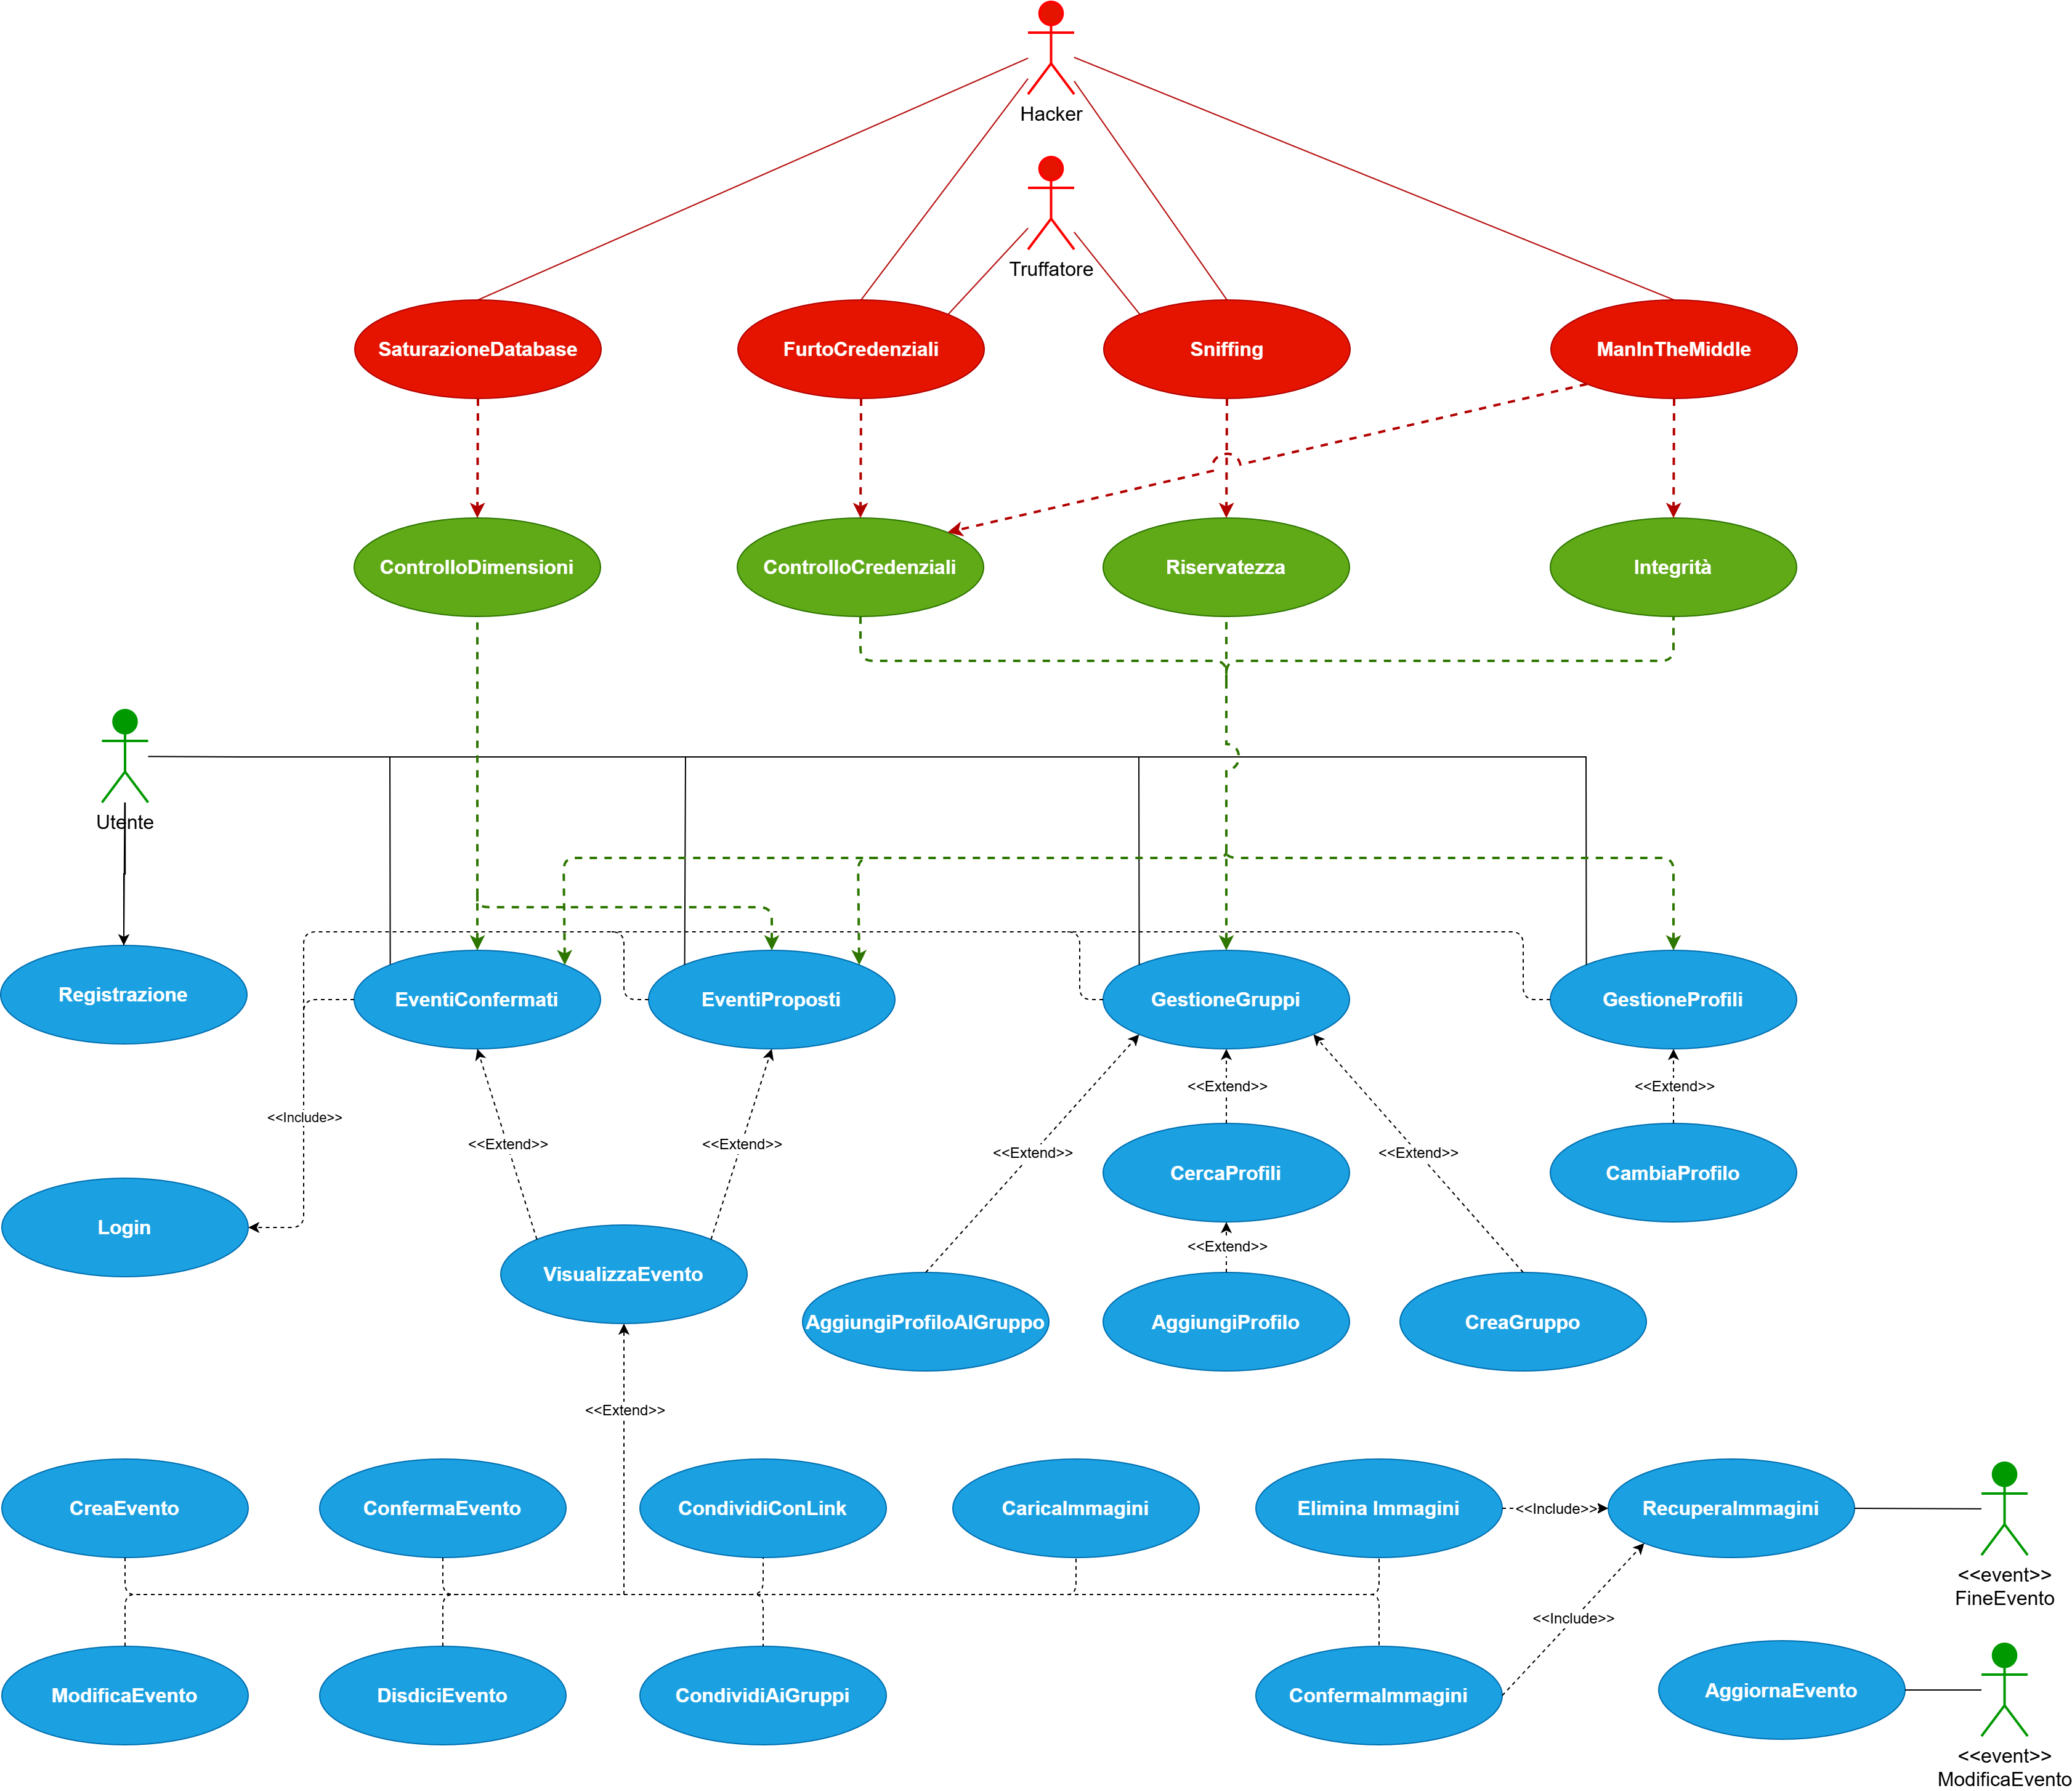
\includegraphics[width=\textwidth]{SecurityCase.png}
        \caption{Casi d'uso relativi alla sicurezza}
    \end{center}

\end{figure}
\clearpage

Visti i costi ed appurate le risorse a disposizione sussistono quindi i seguenti requisiti 
inerenti alla protezione dei dati e delle funzionalità di Wyd:
\begin{enumerate}
    \item Implementare un sistema di log per tracciare tutti i messaggi tra i client e i server, inclusi gli accessi, le richieste di prenotazione, di conferma, di sospensione e di invio e ricezione di dati
    \item I dati salvati devono essere protetti da un attaccante che abbia accesso al sistema, prendendo misure di sicurezza fisica, eventualmente cifrando i dati
    \item I dati inviati tra le parti remote devono essere protetti, utilizzando la cifratura dei dati
    \item Tutte le azioni avvenute sul sistema devono essere tracciate tramite un sistema di log.
    \item Il sistema deve essere resistente ad un alto numero di richieste contemporanee
    \item La dimensione delle richieste non deve superare una determinata soglia
\end{enumerate}

La visione e l'analisi dei log verrà gestita con uno strumento esterno, accessibile solo al personale autorizzato.


\begin{table}[htbp]
    \centering
    \begin{tabular} {|P{1.3cm}|P{11.2cm}|P{3cm}|}
        \hline
        \textbf{ID}                       & \textbf{Requisiti}                                                  & \textbf{Tipo} \\
        \hline
        R21F                              & Implementazione di un sistema di log per tracciare tutti i messaggi
        tra i client e i server           & Funzionale                                                                          \\
        \hline
        R22F                              & Le richieste non devono superare una certa dimensione               & Funzionale    \\
        \hline
        R7NF                              & I dati salvati devono essere protetti da un attaccante che abbia
        accesso al sistema, prendendo misure di sicurezza fisica, eventualmente
        cifrando i dati                   & Non Funzionale                                                                      \\
        \hline
        R8NF                              & I dati inviati tra le parti remote devono essere protetti, utilizzando la cifratura dei dati & Non Funzionale                                                                      \\
        \hline
        R9NF & Il sistema deve essere resistente ad un alto numero di richieste contemporanee & Non funzionale  \\
        \hline
    \end{tabular}
    \caption{Requisiti di sicurezza}
\end{table}

\clearpage
\subsection{L’analisi del problema}

Una volta identificati i requisiti ed i casi d'uso, si procede con l'analisi del problema.\\
\\
L'analisi del problema entra nel merito del comportamento dell'applicazione,
 evidenziando il rapporto tra requisiti, casi d'uso e funzionalità.
Determina quindi l'architettura logica, che delinea le relazioni fondamentali del sistema, 
individuando i componenti logici principali e le loro responsabilità.\\

\subsubsection{Analisi delle funzionalità}
Le funzionalità sono dedotte dai casi d'uso, sintetizzando i servizi principali dell'applicazione.
In particolare, le funzionalità vengono rilevate in base alla loro relazione con gli agli casi d'uso,
alla specificità del compito che assolvono e alla pertinenza reciproca.\\
\\
Si riportano in tabella le funzionalità che racchiudono altri casi d'uso.

\begin{table}[htb]
    \centering
    \begin{tabular} {|P{7.3cm}|P{8cm}|}
        \hline
        \textbf{Funzionalità} & \textbf{Scomposizione}                                                                                                                            \\
        \hline
        EventiConfermati      & VisualizzaEvento                                                                                                                                  \\
        \hline
        EventiProposti        & VisualizzaEvento                                                                                                                                  \\
        \hline
        VisualizzaEvento      & CreaEvento, ModificaEvento, ConfermaEvento, DisdiciEvento, CondividiConLink, CondividiAiGruppi, CaricaImmagini, EliminaImmagini, ConfermaImmagini \\
        \hline
        GestioneGruppi        & CercaProfili, AggiungiProfiloAlGruppo, CreaGruppo                                                                                                 \\
        \hline
        CercaProfili          & AggiungiProfilo                                                                                                                                   \\
        \hline
        GestioneProfili       & CambiaProfilo                                                                                                                                     \\
        \hline
    \end{tabular}
    \caption{Scomposizione delle funzionalità}

\end{table}

\clearpage

Di ogni funzionalità vengono evidenziati il grado di complessità, la tipologia di azione che svolgono ed i requisiti collegati.
Il grado di complessità riassume la quantità e la difficoltà implementativa delle azioni che una funzionalità ricopre.
La tipologia riporta in maniera generale la qualità dei servizi offerti.
Infine si riportano gli identificatori dei requisiti funzionali che ogni finzionalità soddisfa.\\

\begin{table}[htbp]
    \centering
    \begin{tabular} {|P{3.8cm}|P{4.5cm}|P{2.5cm}|P{4cm}|}
        \hline
        \textbf{Funzionalità} & \textbf{Tipo}                                                 & \textbf{Grado di complessità} & \textbf{Requisiti Collegati}                    \\
        \hline
        Login                 & Interazione esterno e lettura dati                            & semplice                      & R2F                                             \\
        \hline
        Registrazione         & Interazione esterno e memorizzazione dati                     & semplice                      & R1F                                             \\
        \hline
        EventiConfermati      & Interazione esterno e gestione dati                           & complessa                     & R3F, R8F                                        \\
        \hline
        EventiProposti        & Interazione esterno e gestione dati                           & complessa                     & R4F, R9F                                        \\
        \hline
        GestioneGruppi        & Interazione esterno e gestione dati                           & complessa                     & R15F, R16F                                      \\
        \hline
        GestioneProfili       & Interazione esterno e gestione dati                           & complessa                     & R17F, R18F, R19F                                \\
        \hline
        VisualizzaEvento      & Interazione esterno e gestione, lettura e memorizzazione dati & complessa                     & R5F, R6F, R7F, R8F, R9F, R10F, R11F, R12F, R14F \\
        \hline
        AggiornaEvento        & Gestione dati                                                 & complessa                     & R20F                                            \\
        \hline
        RecuperaImmagini      & Lettura dati                                                  & complessa                     & R13F                                            \\
        \hline
        ScritturaLog          & Memorizzazione dati                                           & semplice                      & R21F                                            \\
        \hline
    \end{tabular}

    \caption{Funzionalità}
\end{table}
Si procede analizzando i dati che ogni funzionalità gestisce, indicandone la tipologia, la protezione richesta ed i vincoli correlati,
per conoscere in maniera definitiva tutte le caratteristiche delle informazioni scambiate.
A seguito dell'analisi delle informazioni, si procede con l'analisi dei vincoli,
in cui si chiarificano i requisiti non funzionali, evidenziandone le criticità e quali componenti ne vengono coinvolti.

\begin{table}[htbp]
    \centering
    \begin{tabular} {|P{3.5cm}|P{2cm}|P{3.5cm}|P{6cm}|}
        \hline
        \textbf{Requisito}                  & \textbf{Categorie} & \textbf{Impatto}                                                         & \textbf{Funzionalità}                                                                                                                       \\
        \hline
        Semplicità dell'interfaccia         & Usabilità          & Intuitività di utilizzo                                                  & Login, Registrazione, EventiConfermati, EventiProposti, GestioneGruppi, GestioneProfili, VisualizzaEvento, RecuperaImmagini                 \\
        \hline
        Velocità della ricerca dei dati     & Tempo di Risposta  & Maggiore reattività                                                      & EventiConfermati, EventiProposti, GestioneGruppi, GestioneProfili, RecuperaImmagini                                                         \\
        \hline
        Velocità di memorizzazione dei dati & Tempo di Risposta  & Maggiore reattività                                                      & Registrazione, AggiornaEvento, RecuperaImmagini                                                                                             \\
        \hline
        Controllo Accessi                   & Sicurezza          & Peggiorano tempo di risposta e usabilità, migliorano la privacy dei dati & EventiConfermati, EventiProposti, GestioneGruppi, GestioneProfili, VisualizzaEvento                                                         \\
        \hline
        Protezione dei\linebreak Dati       & Sicurezza          & Peggiorano tempo di risposta, migliorano la privacy dei dati             & Login, Registrazione, EventiConfermati, EventiProposti, GestioneGruppi, GestioneProfili, VisualizzaEvento, AggiornaEvento, RecuperaImmagini \\
        \hline
        Scalabilità delle richieste         & Tempo di Risposta  & Minor degradamento delle prestazioni                                     & EventiConfermati, EventiProposti, AggiornaEvento, RecuperaImmagini                                                                          \\
        \hline
    \end{tabular}
    \caption{Vincoli}
\end{table}
\clearpage

Infine si definiscono logicamente le maschere, ovvero i componenti visuali essenziali del programma.
Ad ogni maschera corrisponderà un'interfaccia grafica tramite la quale l'utente potrà accedere alle funzionalità.
Vengono quindi associate le maschere alle funzionalità di cui permettono l'esecuzione, indicando le informazioni relative.

\begin{table}[htbp]
    \centering
\begin{tabular} {|P{4.5cm}|P{6.5cm}|P{4cm}|}
    \hline
    \textbf{Maschera}     & \textbf{Informazioni}                                                                                                              & \textbf{Funzionalità}              \\
    \hline
    View Login            & email, password                                                                                                                    & Login                              \\
    \hline
    View Registrazione    & email, password                                                                                                                    & Registrazione                      \\
    \hline
    View EventiConfermati & lista eventi confermati                                                                                                            & EventiConfermati, AggiornaEvento   \\
    \hline
    View EventiProposti   & lista eventi proposti                                                                                                              & EventiProposti, \linebreak AggiornaEvento     \\
    \hline
    View VisualizzaEvento & Identificativo utente, titolo, descrizione, data e orario di inizio, data e orario di fine, confermato, immagini, profili associati & VisualizzaEvento, RecuperaImmagini \\
    \hline
    View GestioneGruppi   & lista gruppi                                                                                                                       & GestioneGruppi                     \\
    \hline
    View CercaProfili     & tag di ricerca, lista profili                                                                                                      & CercaProfili                       \\
    \hline
    View GestioneProfili  & Lista profili, Identificativo utente, Identificativo profilo corrente                                                              & GestioneProfili                    \\
    \hline
\end{tabular}
\caption{Maschere}
\end{table}

\clearpage




\subsubsection{Architettura logica}


Definite le relazioni e le informazioni relative alle funzionalità, 
si necessita di esprimere logicamente i componenti principali del prodotto e le loro relazioni.
Le funzionalità vengono espresse a livello logico tramite package e diagrammi delle classi, 
mentre i dati vengono descritti all'interno del dominio. \\
\\
Il modello del dominio individua le entità che rappresentano logicamente le dipendenze tra i dati.
Ogni entità presenta i suoi dati tramite proprietà, identificate da un nome e dalla tipologia del dato.
Inoltre, all'interno del modello vengono indicati i rapporti tra le entità specificando le cardinalità reciproche.\\

\begin{figure}[h!]
    \begin{center}
        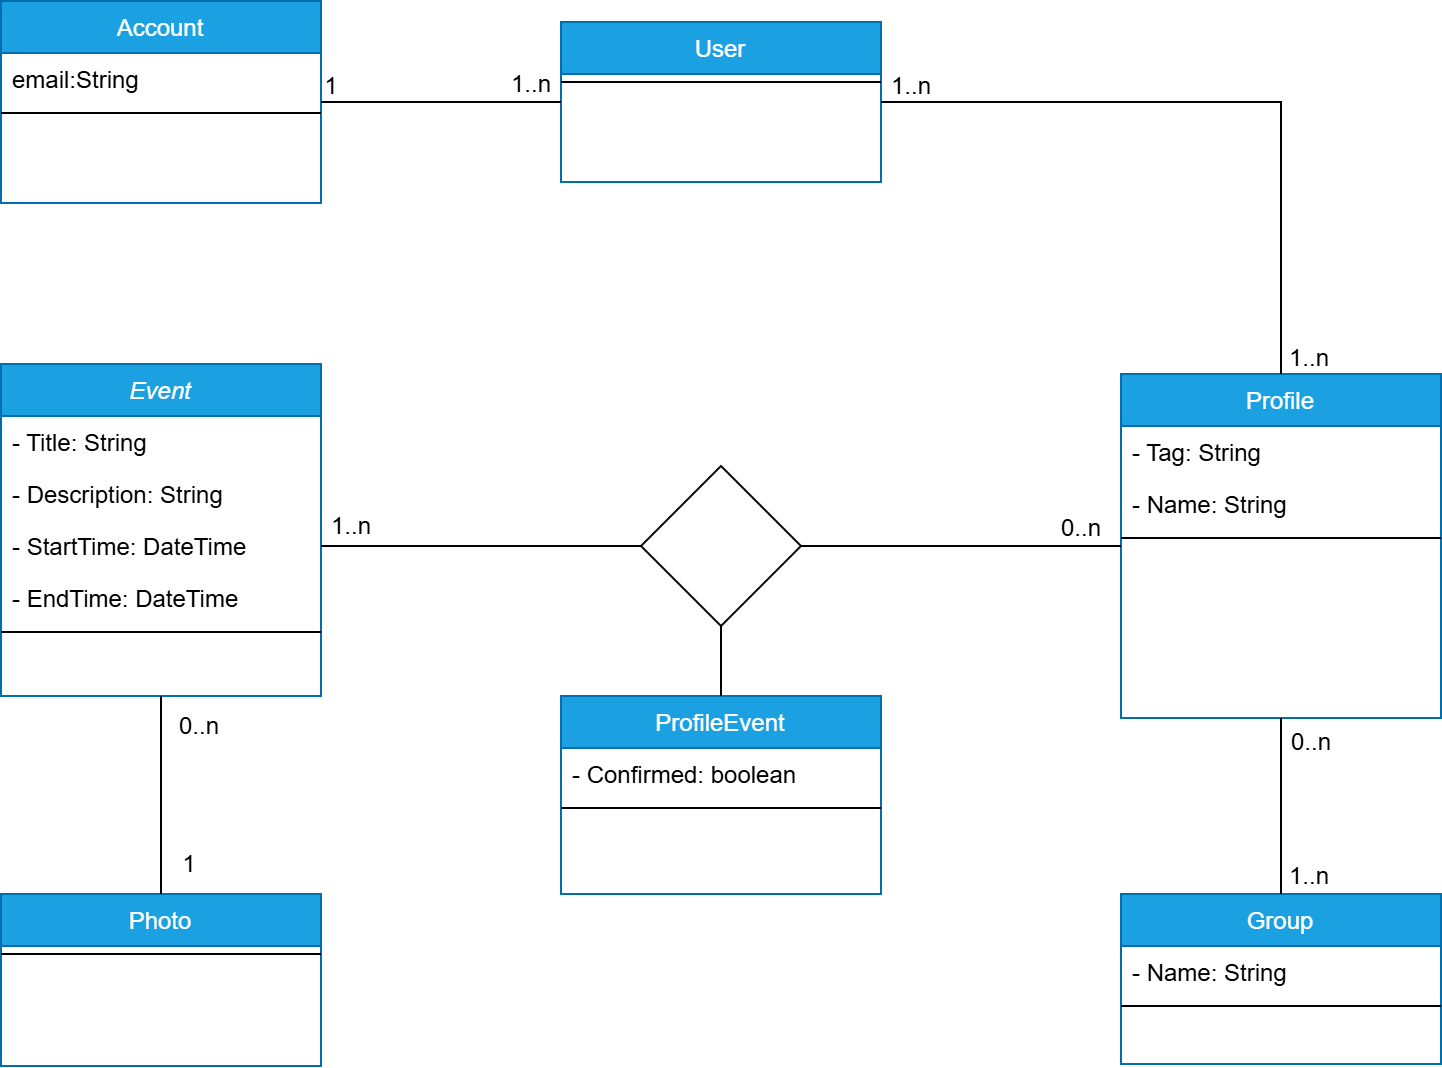
\includegraphics[width=\textwidth]{ModelloDominio.png}
        \caption{Modello del dominio}
    \end{center}
\end{figure}
\clearpage


La divisione delle responsabilità logiche viene descritta nel diagramma dei package.
Ogni package rappresenta una parte di prodotto che soddisfa una determinata responsabilità. 
La responsabilità viene individuata in base alla peculierità ed alle dipendenze delle funzionalità che ricopre.
Si possono così distinguere, ad esempio, package relativi a interfacce grafiche, logiche applicative o gestione della persistenza, 
in base alle caratteristiche specifiche del prodotto.
Il diagramma dei package offre una prima struttura delle parti del progetto e del loro rapporto.\\
\\

\begin{figure}[h!]
    \begin{center}
        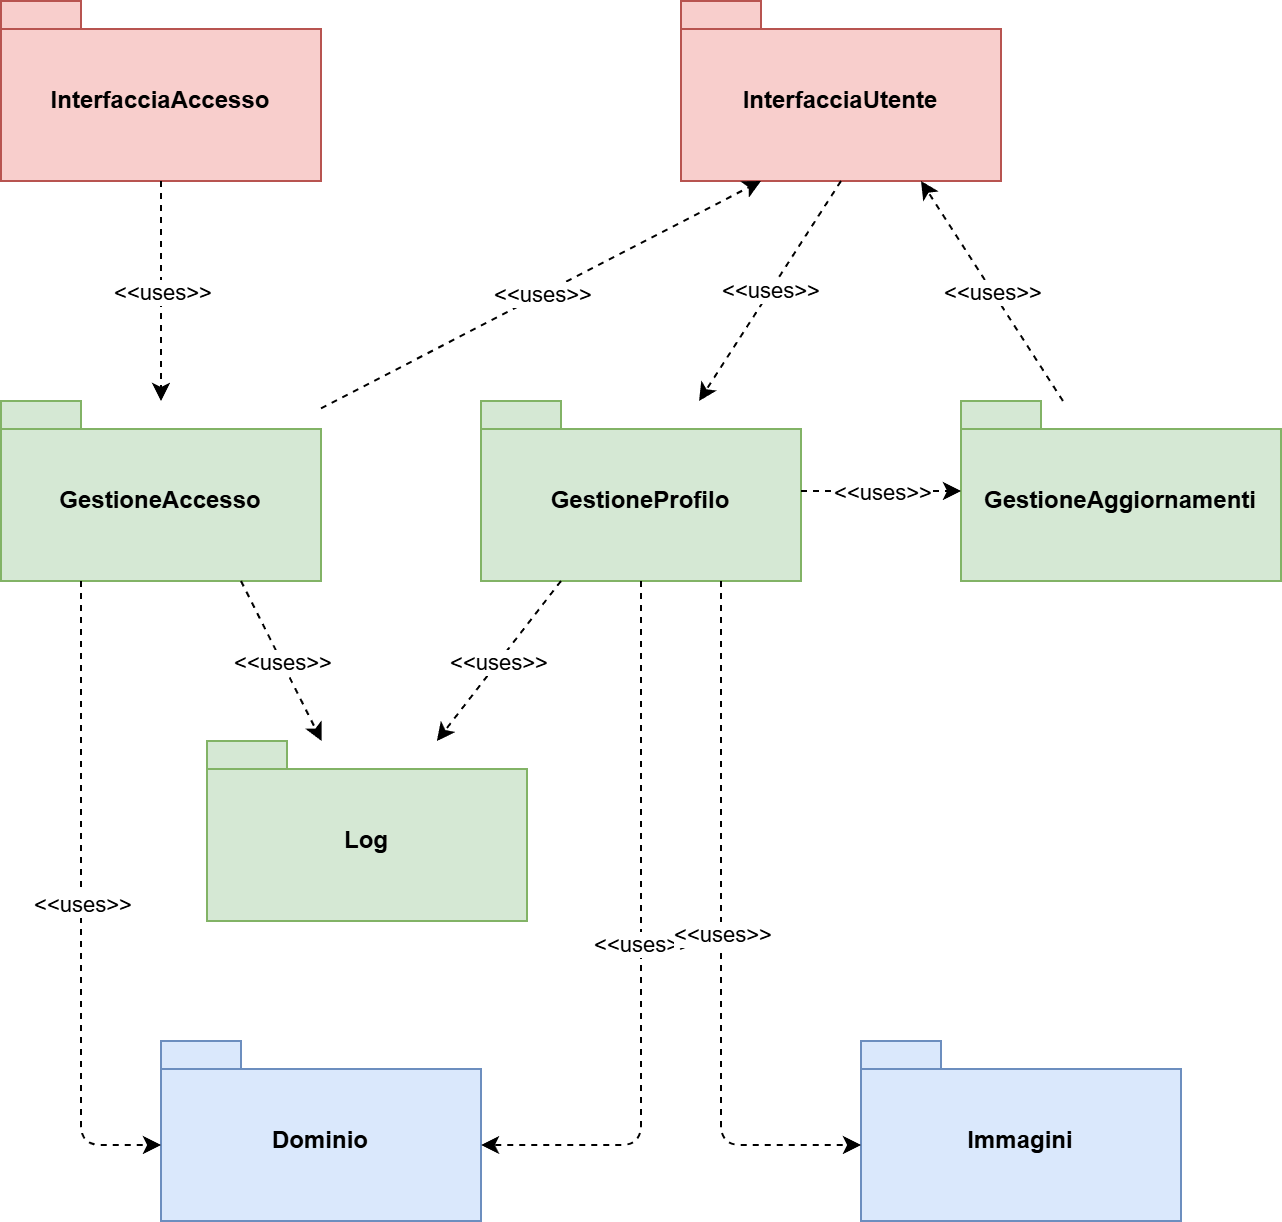
\includegraphics[width=\textwidth]{DiagrammaPackage.png}
        \caption{Diagramma dei Package}
    \end{center}
\end{figure}
\clearpage

Ogni package contiene una o più classi che lo implementano.
Ogni classe rappresenta un componente logico che assume uno specifico scopo.
Le classi possono presentare dei metodi, ovvero delle istanze che descrivono le funzionalità fornite,
alle quali altri componenti possono fare richiesta di esecuzione.
La definizione delle classi permette di creare una struttura iniziale presentando le funzionalità minime e 
le dipendenze tra le parti.

\begin{figure}[h!]
    \begin{center}
        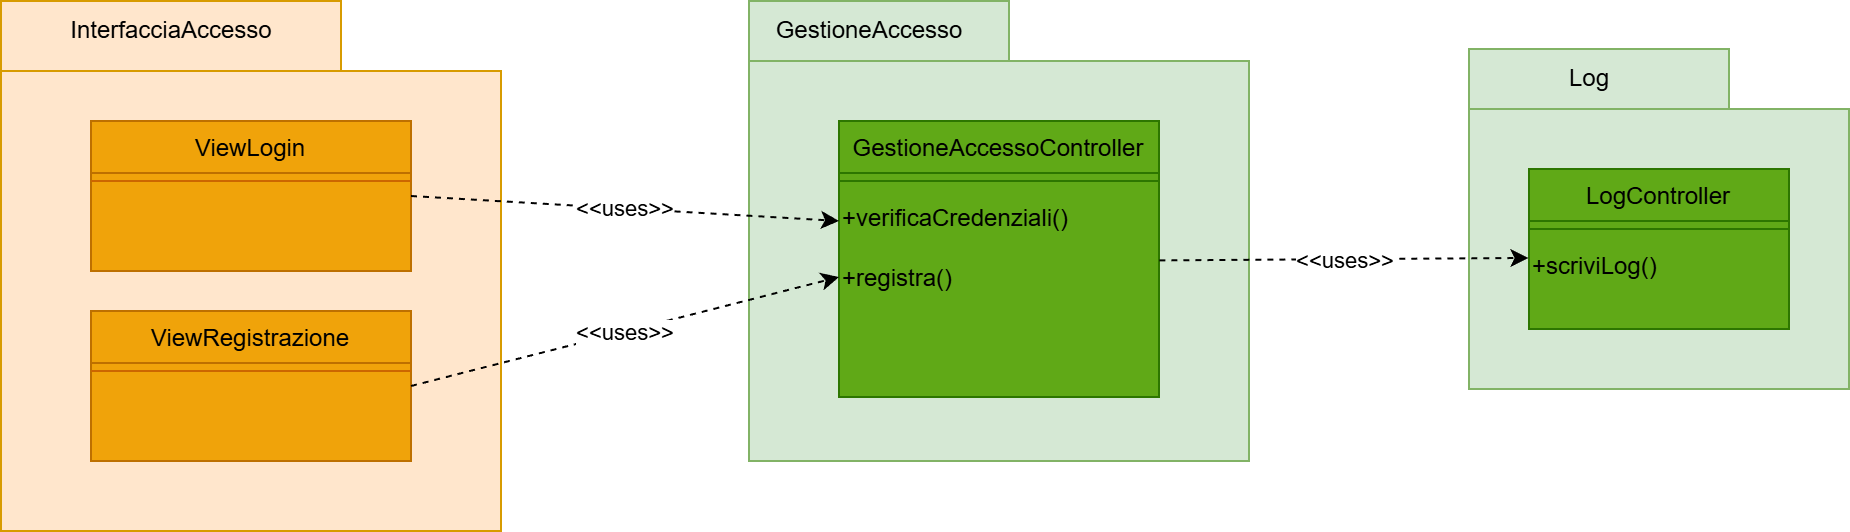
\includegraphics[height=0.18\textheight]{GestioneAccesso.png}
        \caption{Diagramma delle classi: interfacca e gestione accesso}
    \end{center}
\end{figure}


\begin{figure}[h!]
    \begin{center}
        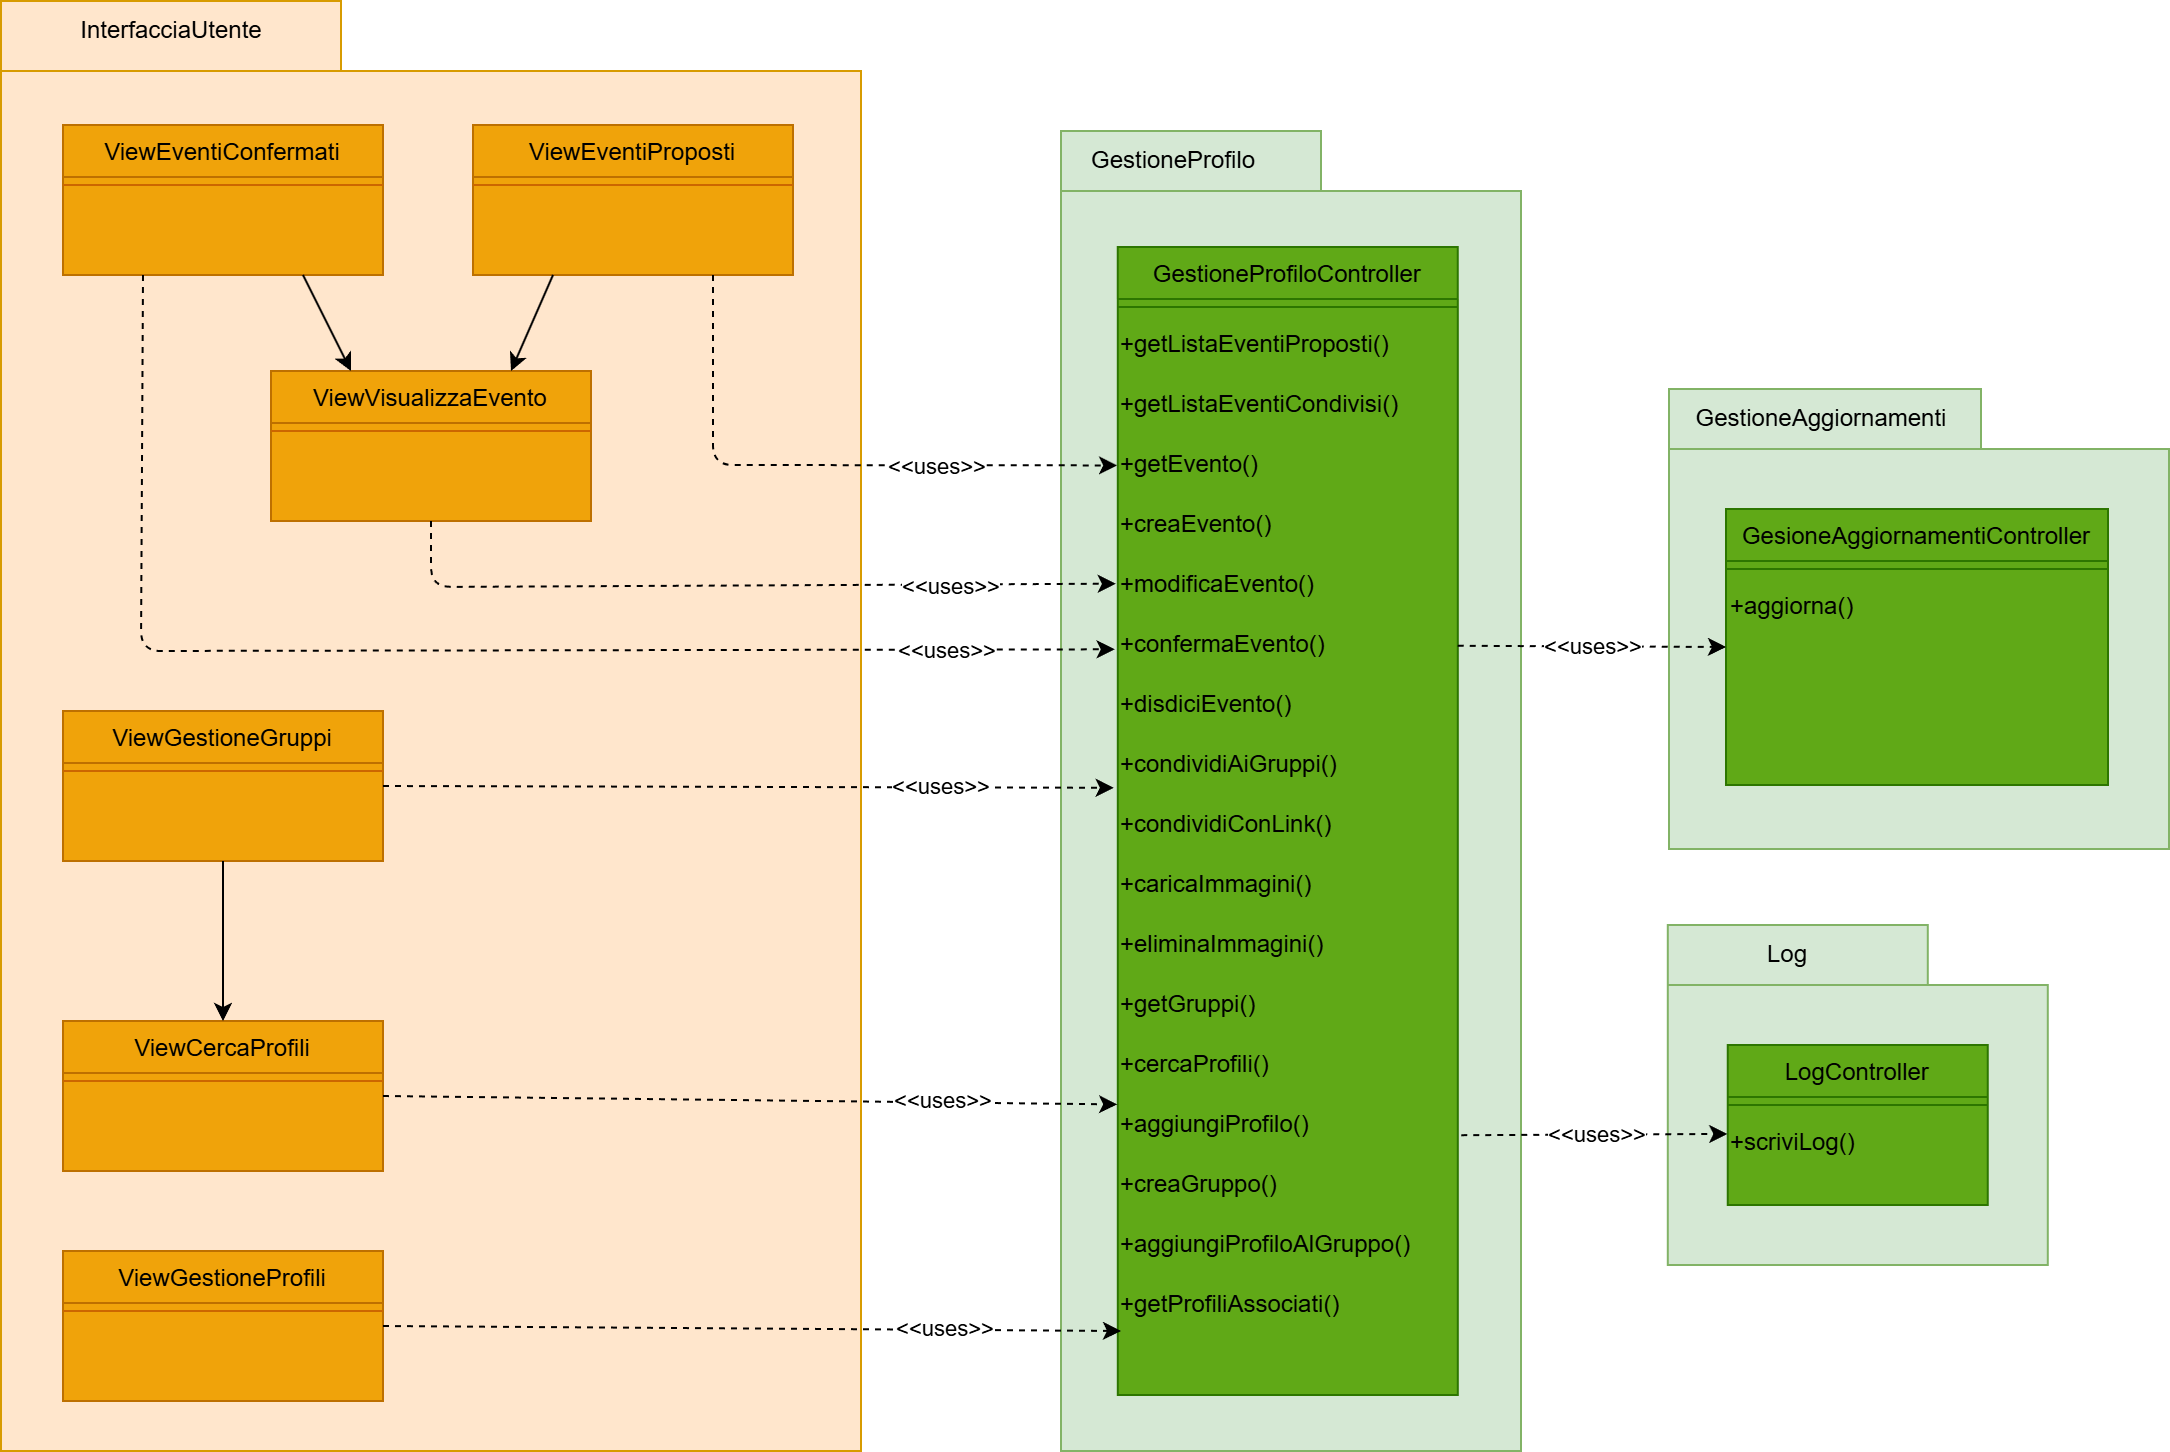
\includegraphics[height=0.425\textheight]{GestioneProfilo.png}
        \caption{Diagramma delle classi: interfacca utente, gestione profilo ed aggiornamenti}
    \end{center}
\end{figure}
\clearpage
\section{Struttura centrale}

Lo sviluppo di un’applicazione segue un processo strutturato, articolato in diverse fasi. In fase di progettazione,
l'obiettivo principale è identificare le caratteristiche funzionali e comportamentali del sistema, delineando le componenti principali e le rispettive responsabilità.
Questa fase permette di definire un'architettura coerente, facilitando le successive scelte tecnologiche e implementative.\\
\\
Nella fase successiva, di implementazione, si procede con il passaggio dall’analisi teorica alla realizzazione concreta,
dove la selezione dell’architettura e delle tecnologie di riferimento assumono un ruolo centrale.
Le decisioni prese in questa fase determinano il comportamento dei diversi componenti e le modalità con cui essi interagiscono tra loro.
Un’attenta selezione delle soluzioni ottimali, più adatte ai requisiti definiti in fase di progettazione,
permette di impostare fin dalle prime iterazioni uno sviluppo efficiente e strutturato, minimizzando la necessità di revisioni successive.\\
\\
Mentre alcune decisioni risultano immediate o intercambiabili, altre richiedono analisi approfondite per individuare la soluzione più adatta.
Un approccio efficace consiste nello sviluppare inizialmente i componenti con requisiti ben definiti,
per poi affinare progressivamente l'integrazione e la configurazione degli altri elementi del sistema.
L'identificazione, anche parziale, di una struttura iniziale consente di delineare i vincoli di integrazione e di semplificare la definizione delle soluzioni residue.\\
\\
L’architettura dell’applicativo si basa su una chiara suddivisione in componenti, ciascuno con un ruolo specifico all’interno del sistema.
L'interfaccia grafica è responsabile della presentazione e dell’interazione con l’utente, ponendo particolare attenzione alla coerenza visiva e alla fluidità dell’esperienza.\\
\\
La logica applicativa viene gestita da un server centrale, il quale si occupa di coordinare le comunicazioni tra i diversi servizi e di garantire il corretto flusso delle operazioni.
La gestione dell’autenticazione degli utenti è delegata a un servizio apposito,
che consente di separare questa responsabilità dal resto del sistema, migliorando sia le prestazioni che la sicurezza.\\
\\
Un ulteriore aspetto fondamentale nella progettazione del sistema riguarda la protezione delle comunicazioni e dei dati sensibili.
L’adozione di misure di sicurezza adeguate è essenziale per garantire la protezione delle informazioni scambiate tra i vari componenti e
per ridurre i rischi derivanti da eventuali attacchi esterni.
Inoltre, per monitorare il corretto funzionamento dell’applicazione e identificare tempestivamente eventuali anomalie,
il sistema è integrato con strumenti di logging e analisi delle prestazioni.\\
\\
Questa organizzazione modulare consente di ottimizzare la scalabilità e la manutenibilità dell’applicativo,
facilitando eventuali evoluzioni future.
La suddivisione chiara delle responsabilità, unita a un’architettura flessibile e sicura,
rappresenta quindi un elemento chiave per garantire la stabilità e l’efficienza del sistema nel lungo periodo.\\
\\

\begin{figure}[h!]
    \centering
    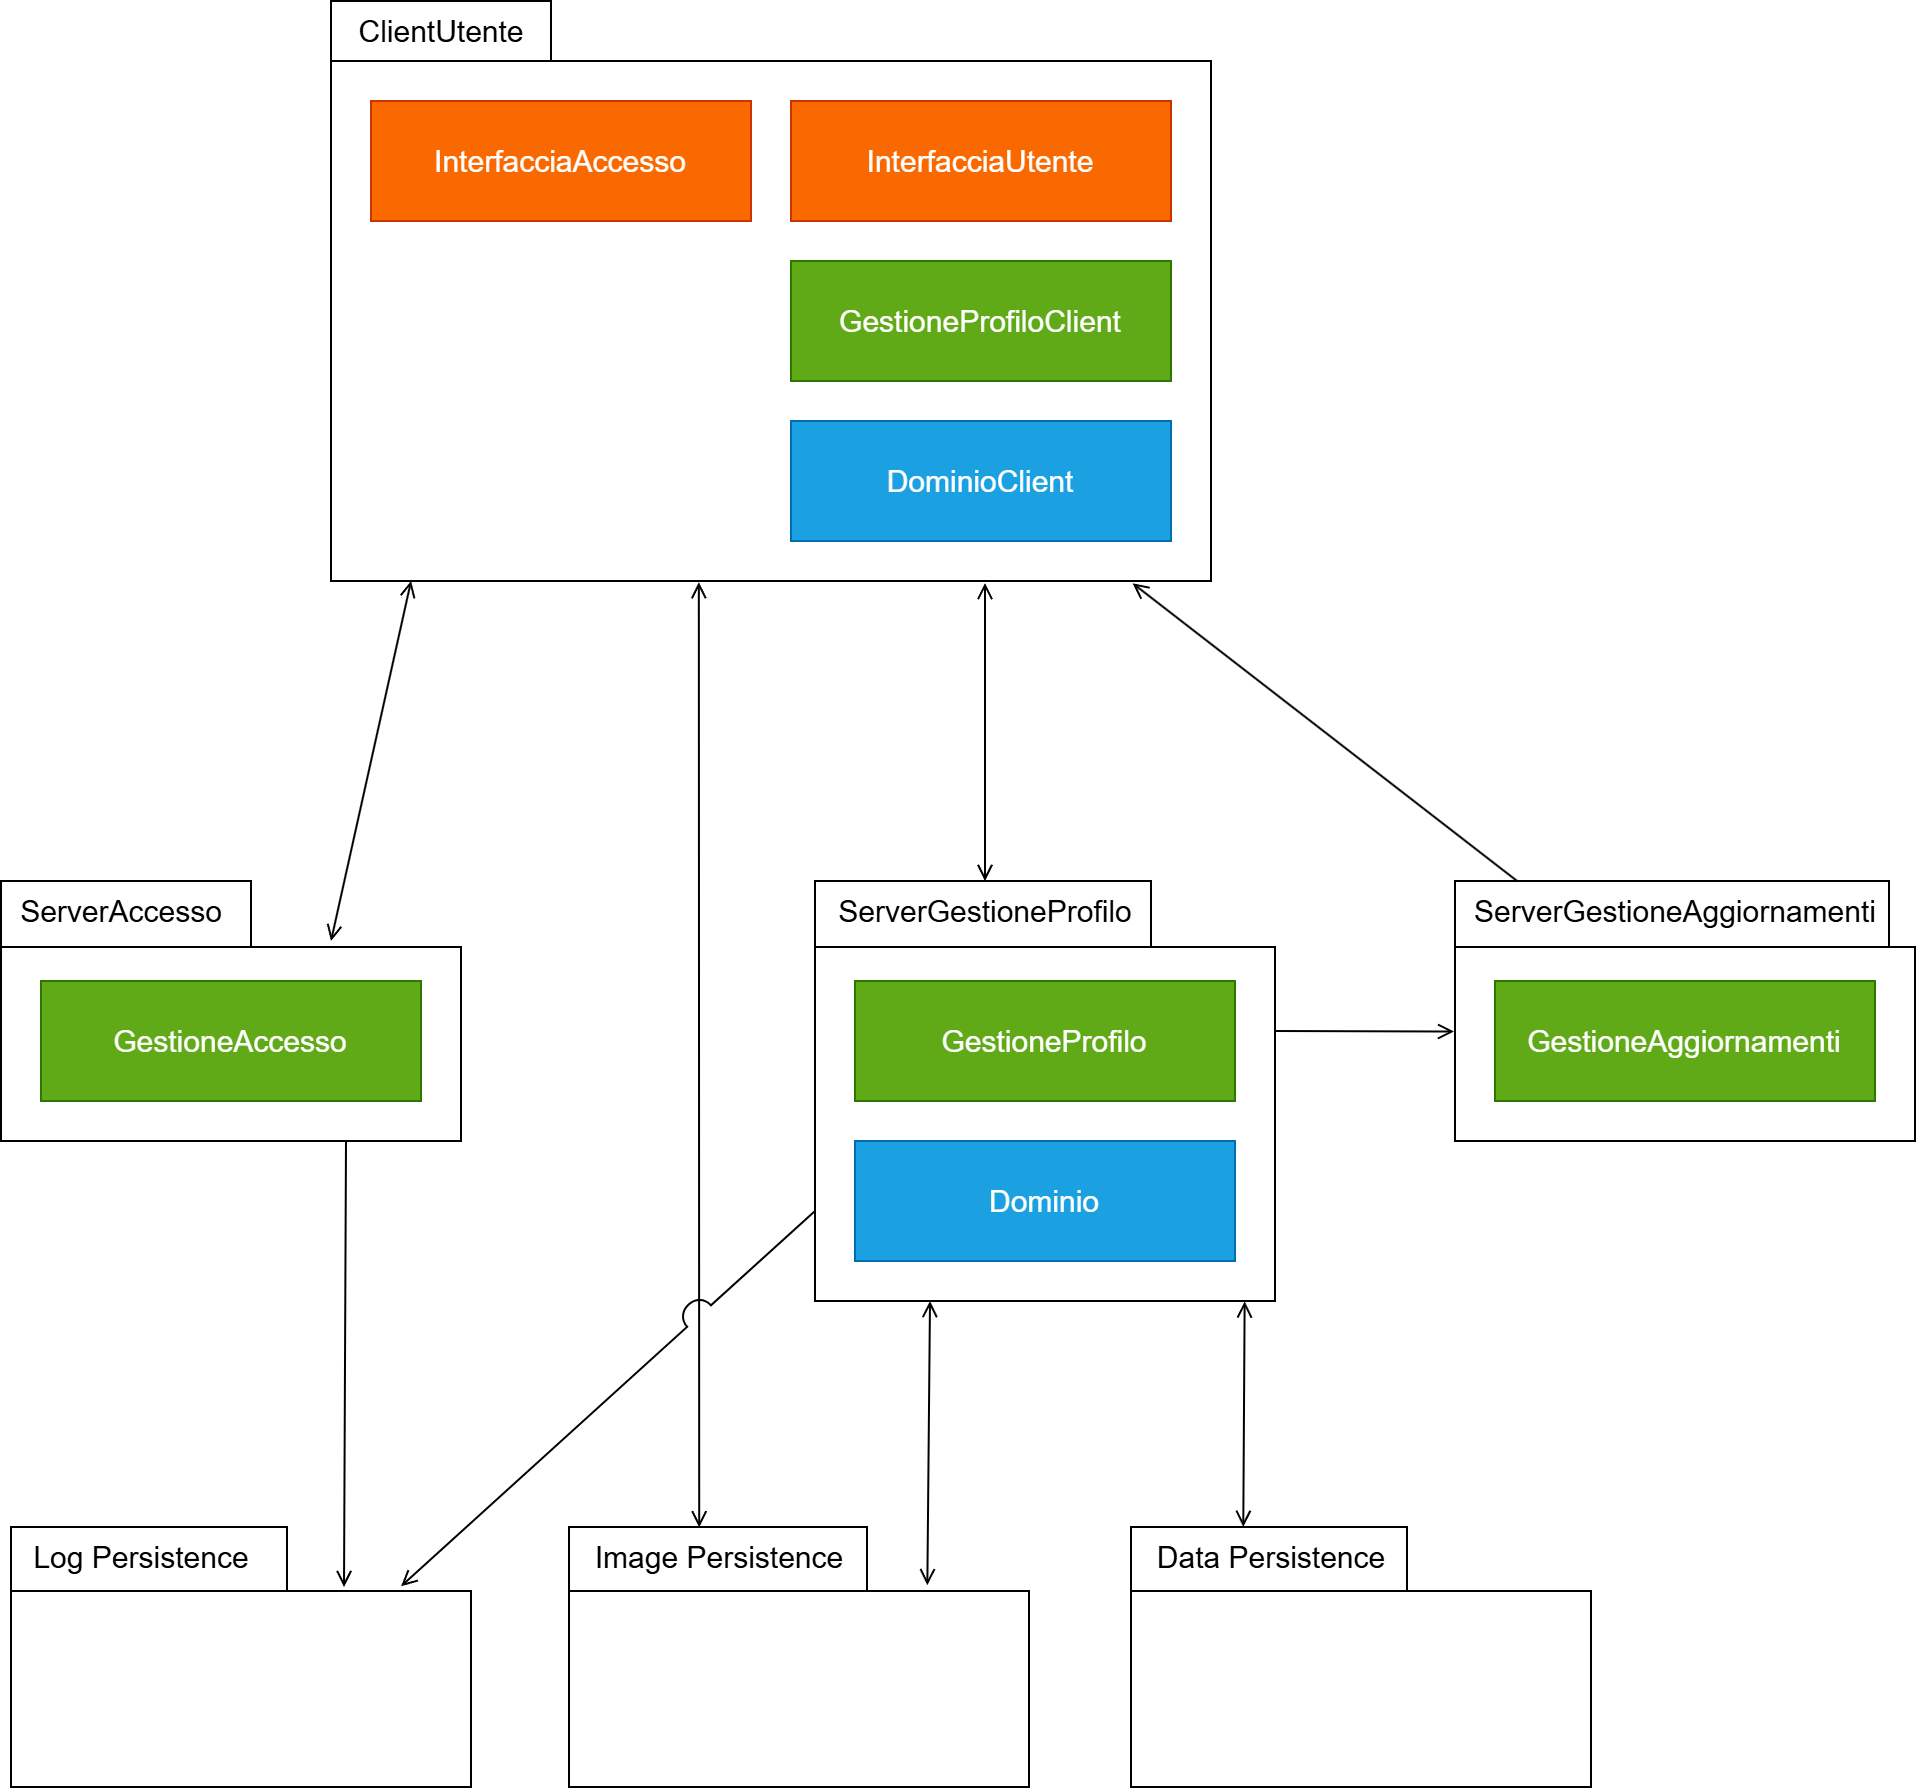
\includegraphics[width=\textwidth]{ProgettoDiagrammaPackage.png}
    \caption{Struttura e responsabilità delle parti del progetto}
\end{figure}

\clearpage
\subsection{Lo sviluppo dell'applicazione utente}

L’utilizzo delle applicazioni per la gestione degli eventi può essere suddiviso in due fasi distinte, 
ciascuna con specifiche esigenze funzionali.\\
La prima fase riguarda infatti la pianificazione a lungo termine e l’organizzazione degli impegni.
In questa circostanza l’utente decide come distribuire il proprio tempo, pianificando attività e appuntamenti,
e strutturando il proprio calendario nel modo più efficiente per le proprie necessità.
La seconda fase riguarda invece la gestione degli eventi non ancora certi e definiti;
ciò include l’invito a un evento, l’eventuale conferma da parte dell’utente,
l’identificazione degli impegni a breve termine e l’aggiornamento del loro stato
(ad esempio, se l’evento sia ancora confermato, quante persone vi partecipano, se qualcuno ha annullato o se l'evento è già concluso)
con la gestione degli eventuali contenuti multimediali successivi all’evento. Queste due fasi implicano un approccio diverso da parte dell’utente,
comportando di conseguenza esigenze differenti a cui l’applicazione deve rispondere adeguatamente.\\
\\
Per rispondere a tali necessità, è fondamentale che l'applicazione offra un'interfaccia utente versatile, fruibile sia da desktop che da dispositivi mobili.
La versione desktop consente una pianificazione a lungo termine, offrendo una visione d'insieme chiara e completa di tutti gli impegni,
tale da facilitare la gestione del tempo.
D'altra parte, la versione mobile deve permettere una gestione rapida e dinamica degli eventi quotidiani,
garantendo che l'utente possa rimanere sempre connesso e aggiornato sugli sviluppi in tempo reale.\\
\\
Inoltre, considerando che l'applicazione è destinata a un utilizzo diffuso e a un'utenza potenzialmente elevata,
è necessario garantire tempi di risposta ridotti e una gestione efficiente delle richieste concorrenti.
Ciò implica la progettazione di un sistema in grado di scalare facilmente,
per supportare un ampio numero di utenti simultanei senza compromettere le prestazioni.\\
\\
Già consolidata e affidabile, sin dalle prime fasi di sviluppo del progetto è stata adottata la piattaforma cloud Azure, per garantire un'infrastruttura solida e scalabile.
\clearpage


\subsubsection{Il framework di sviluppo}
Al fine di ottenere tutte le prestazioni precedentemente elencate, 
la scelta è ricaduta sull’adozione del framework di sviluppo Flutter.
Diversi fattori motivano tale decisione. \\
\\
In primo luogo, l'architettura di Flutter si basa su un motore grafico indipendente dalla piattaforma di esecuzione,
il che consente di ottenere elevate prestazioni e garantire un'esperienza utente uniforme su dispositivi diversi. \\
In secondo luogo, Flutter adotta un approccio dichiarativo nella progettazione dell'interfaccia grafica,
che facilita lo sviluppo di componenti reattivi attraverso un codice conciso, facilmente manutenibile.\\
Un ulteriore vantaggio di Flutter è rappresentato dalla crescente adozione nel settore,
dalla solidità della community di sviluppo e dal supporto offerto da Google,
che ne assicurano la stabilità, l'efficienza, la sicurezza e la disponibilità di componenti personalizzabili per l'intero ciclo di vita del prodotto.\\
Infine, Flutter consente uno sviluppo rapido e interattivo grazie alla sua sintassi intuitiva e al meccanismo di hot reload,
che riduce significativamente i tempi di compilazione e facilita il testing in tempo reale.\\
\\
Tra le altre tecnologie valutate per lo sviluppo dell'interfaccia grafica, vi erano React Native e Xamarin.
Tuttavia, entrambe presentano alcune limitazioni: 
le applicazioni finali sviluppate con React Native tendono ad avere dimensioni più elevate e le prestazioni risultano inferiori,
in particolare nella gestione della memoria.
Xamarin, pur essendo una valida opzione, presenta una curva di apprendimento più ripida e 
una comunità di sviluppatori ridotta rispetto a Flutter,
con una conseguente minore disponibilità di componenti e librerie.\\
\\
L'applicazione utente ha come obiettivo la soddisfazione di due compiti principali: interagire con l'utente e 
comunicare con il server, per recuperare i dati e salvare le modifiche apportate.

\clearpage


\subsubsection{Le interfacce grafiche}
L'interazione utente avviene tramite interfacce grafiche 
che permettono di visualizzare i dati e le funzionalità a disposizione. 
Per rispettare il requisito di semplicità e fluidità dell'esperienza è essenziale che 
ogni interfaccia sia il più intuitiva possibile, tramite una limitata varietà di azioni nella stessa pagina,
ognuna delle quali il più riconoscibile e accessibile possibile in base sua importanza e funzionalità.\\
\\
Per ogni maschera individuata in fase di analisi corrisponde almeno un'interfaccia grafica che, 
oltre a gestire la navigazione con le altre interfacce, 
pemette all'utente di eseguire le proprie funzionalità,
esponendo chiaramente le informazioni,
concentrando l'attenzione sui dati eventualmente richiesti e segnalando le azioni eseguibili.\\
\\
Nei diagrammi di dettaglio le interfacce vengono presentate elencando le funzionalità di cui dispongono, 
assieme alle loro relazioni di dipendenza. \\
\\
Si riportano le interfacce di gestione dei gruppi e di visualizzazione degli eventi, 
in quanto funzionalità centrali, il cui stile grafico è stato rispettato nella creazione del resto dell'applicazione.\\
\\
\begin{figure}[htbp]
    \begin{center}
        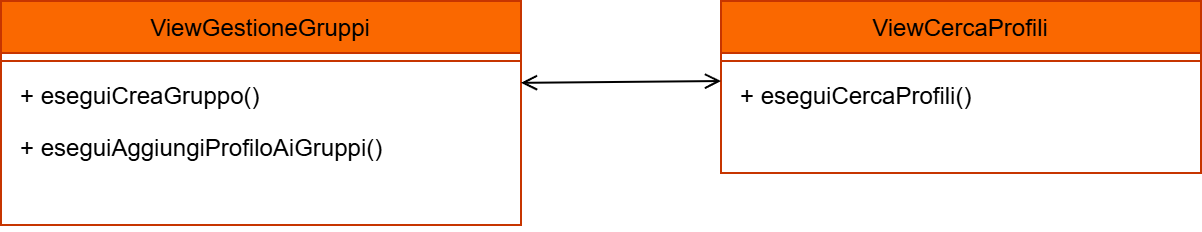
\includegraphics[width=\textwidth]{ProgettoViewGruppi.png}
        \caption{Diagramma di dettaglio delle interfacce di gestione dei gruppi}
    \end{center}
\end{figure}
\clearpage
L'interfaccia di gestione dei gruppi ha il compito di presentare tutti i gruppi associati al profilo attualmente in uso,
fornendo l'accesso alle azioni relative. 
Li elenca quindi in maniera chiara, definendo la differenza tra gruppi di due o più persone.
Per ognuno mostra un bottone dal quale, se selezionato, compariranno le azioni attuabili sul gruppo 
(ad esempio, di aggiungere un profilo).\\
\\
Correlata alla gestione dei profili c'è la loro ricerca, 
che consente il ritrovamento e la sucessiva aggiunta dei profili tra i propri gruppi.
La schermata risulta minimale, consentendo all'utente di concentrarsi sulle sole informazioni e funzionalità essenziali.\\
\\


\mycomment{
TODO immagini gruppi(aggiungi profilo al gruppo)
(crea gruppo)

}
\begin{figure}[htbp]
    \centering
    \begin{subfigure}{0.49\textwidth}
        \centering
        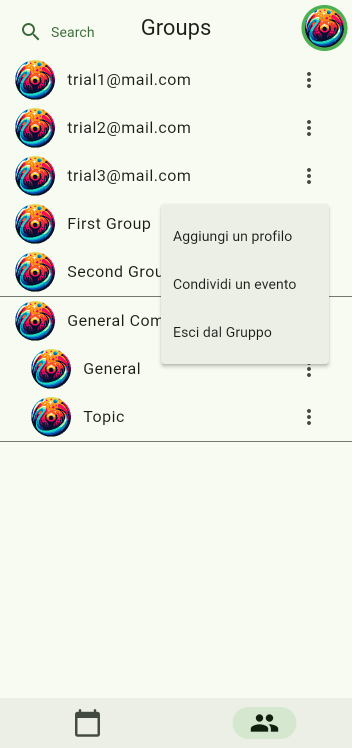
\includegraphics[height=11.5cm, keepaspectratio]{gruppi.png}
        \caption{Elenco dei gruppi}
    \end{subfigure}
    \hfill
    \begin{subfigure}{0.49\textwidth}
        \centering
        
\includegraphics[height=11.5cm, keepaspectratio]{cerca.png}
        \caption{Ricerca dei profili}
    \end{subfigure}
    \caption{Schermate dei gruppi}
\end{figure}


\clearpage

La visualizzazione degli eventi prevede due componenti principali.\\
\\
Il primo consiste in una panoramica generale, affiancando gli eventi tra loro a livello settimanale,
per fornire all'utente un quadro complessivo degli impegni. 
Tale vista è ripetuta sia per gli eventi proposti che per quelli confermati, 
con la possibilità di navigare tra le due schermate.\\
\\
Il secondo entra nel particolare dell'evento, 
mostrando i dettagli relativi e fornendo la possibilità di modificarli. 
Concentra inoltre le principali funzionalità dell'applicazione, 
quali la conferma della partecipazione all'evento, la condivisione con i gruppi e il caricamento delle immagini.\\
\\

\begin{figure}[h!]
    \begin{center}
        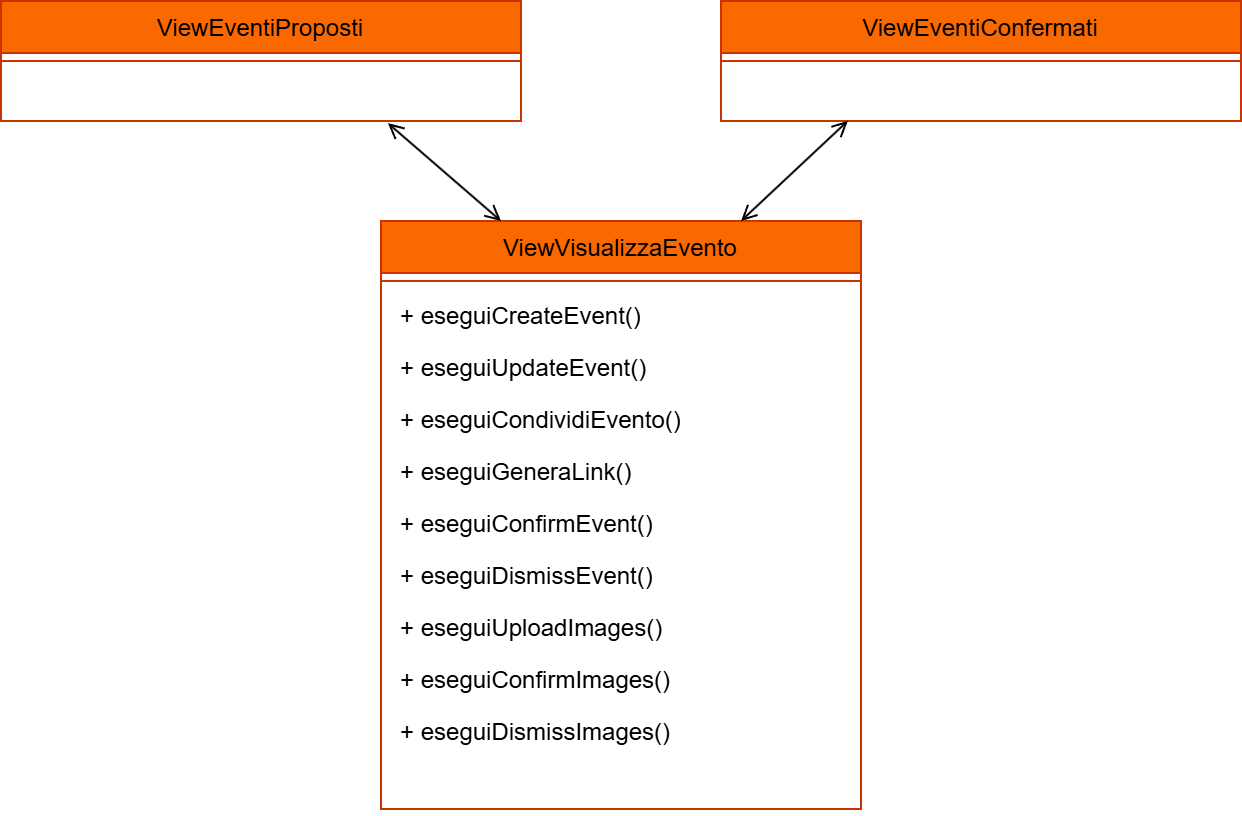
\includegraphics[width=\textwidth]{ProgettoViewEventi.png}
        \caption{Diagramma di dettaglio delle interfacce di visualizzazione eventi}
    \end{center}
\end{figure}
\clearpage

Queste due funzionalità sono al centro del servizio del sistema, 
ed è quindi essenziale che l'interfaccia proposta sia veloce ma sopratutto intuitiva.
Fondamentale in questo riguardo è l'importanza data dai colori, attraverso i quali
ogni elemento risalta in base alla sua importanza, e fornisce il suo contesto e le sue proprietà 
grazie al puro impatto visivo.\\
\\



\begin{figure}[htbp]
    \centering
    \begin{subfigure}{0.49\textwidth}
        \centering
        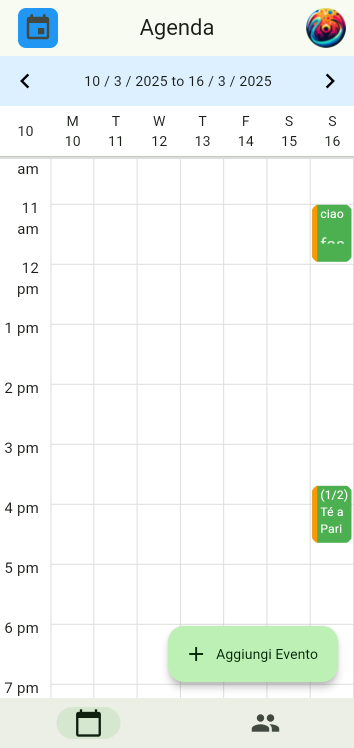
\includegraphics[height=11.5cm, keepaspectratio]{agenda.png}
        \caption{Visualizzazione generale degli eventi}
    \end{subfigure}
    \hfill
    \begin{subfigure}{0.49\textwidth}
        \centering
        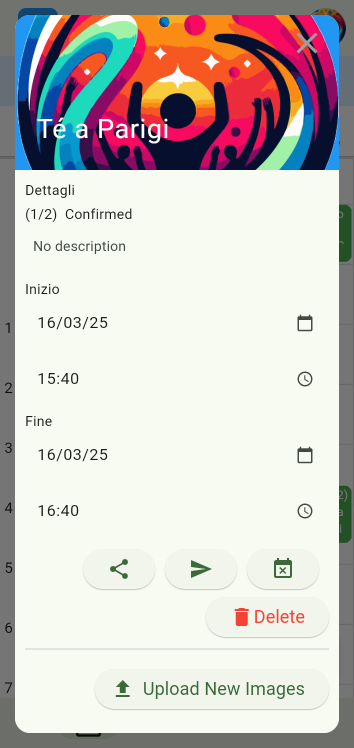
\includegraphics[height=11.5cm, keepaspectratio]{evento.png}
        \caption{Dettaglio di un evento}
    \end{subfigure}
    \caption{Schermate degli eventi}
\end{figure}

\clearpage


\subsubsection{La logica applicativa}

Ogni interazione con l'utente scatena una qualche forma di elaborazione di dati. 
La visualizzazione di qualunque componente comporta il ritrovamento delle infomazioni, 
la loro modifica necessita di essere salvata e la loro condivisione esige la propagazione degli aggiornamenti.
Inoltre, alcuni casi d'uso richiedono azioni da svolgere in autonomia.
L'implementazione della logica necessaria, 
per rispondere efficacemente ai requisiti di velocità ed efficenza,
avviene tramite la creazione di diversi componenti.\\
\\
La suddivisione del programma individua e raggruppa le funzionalità in base al loro contesto, 
affidando ad ogni componente meno responsabilità possibili.
Questo permette di concentrare le logiche condivise, 
evitando duplicazioni e definendo chiaramente il ruolo di ogni metodo.
La semplicità del codice così raggiunta semplifica il futuro sviluppo e la sua manutenzione.\\
\\
La principale suddivisione dei componenti avviene in base agli elementi del dominio.
Per ogni principale entità, infatti, viene creato un servizio che ne racchiude
le richeste di ritrovamento, modifica e salvataggio correlate.
Collegando i servizi al dominio si concentrano anche le eventuali dipendenze da altri servizi, 
riducendole alle sole inerenti all'elemento specifico, 
mantenendo un parallelismo logico anche a livello di relazione.\\
\\
La maggior parte delle richieste che riguardano gli elementi del dominio prevede 
la comunicazione con il server esterno. 
La ricezione e l'aggiornamento dei dati, così come la permanenza delle modifiche, avviene infatti attraverso 
l'interazione con la persistenza principale, a cui si può accedere tramite il server.
Vista la complessità specifica nella creazione delle trasmissioni e 
la loro secondaria importanza a livello logico, 
vengono realizzati dei componenti dedicati, chiamati API.
I componenti API permettono quindi l'astrazione delle trasmissioni con il server, 
semplificando il codice e 
separando la logica applicativa dalle complessità richieste dalla tecnologia dei protocolli usata.

\clearpage 

\begin{figure}[h!]
    \begin{center}
        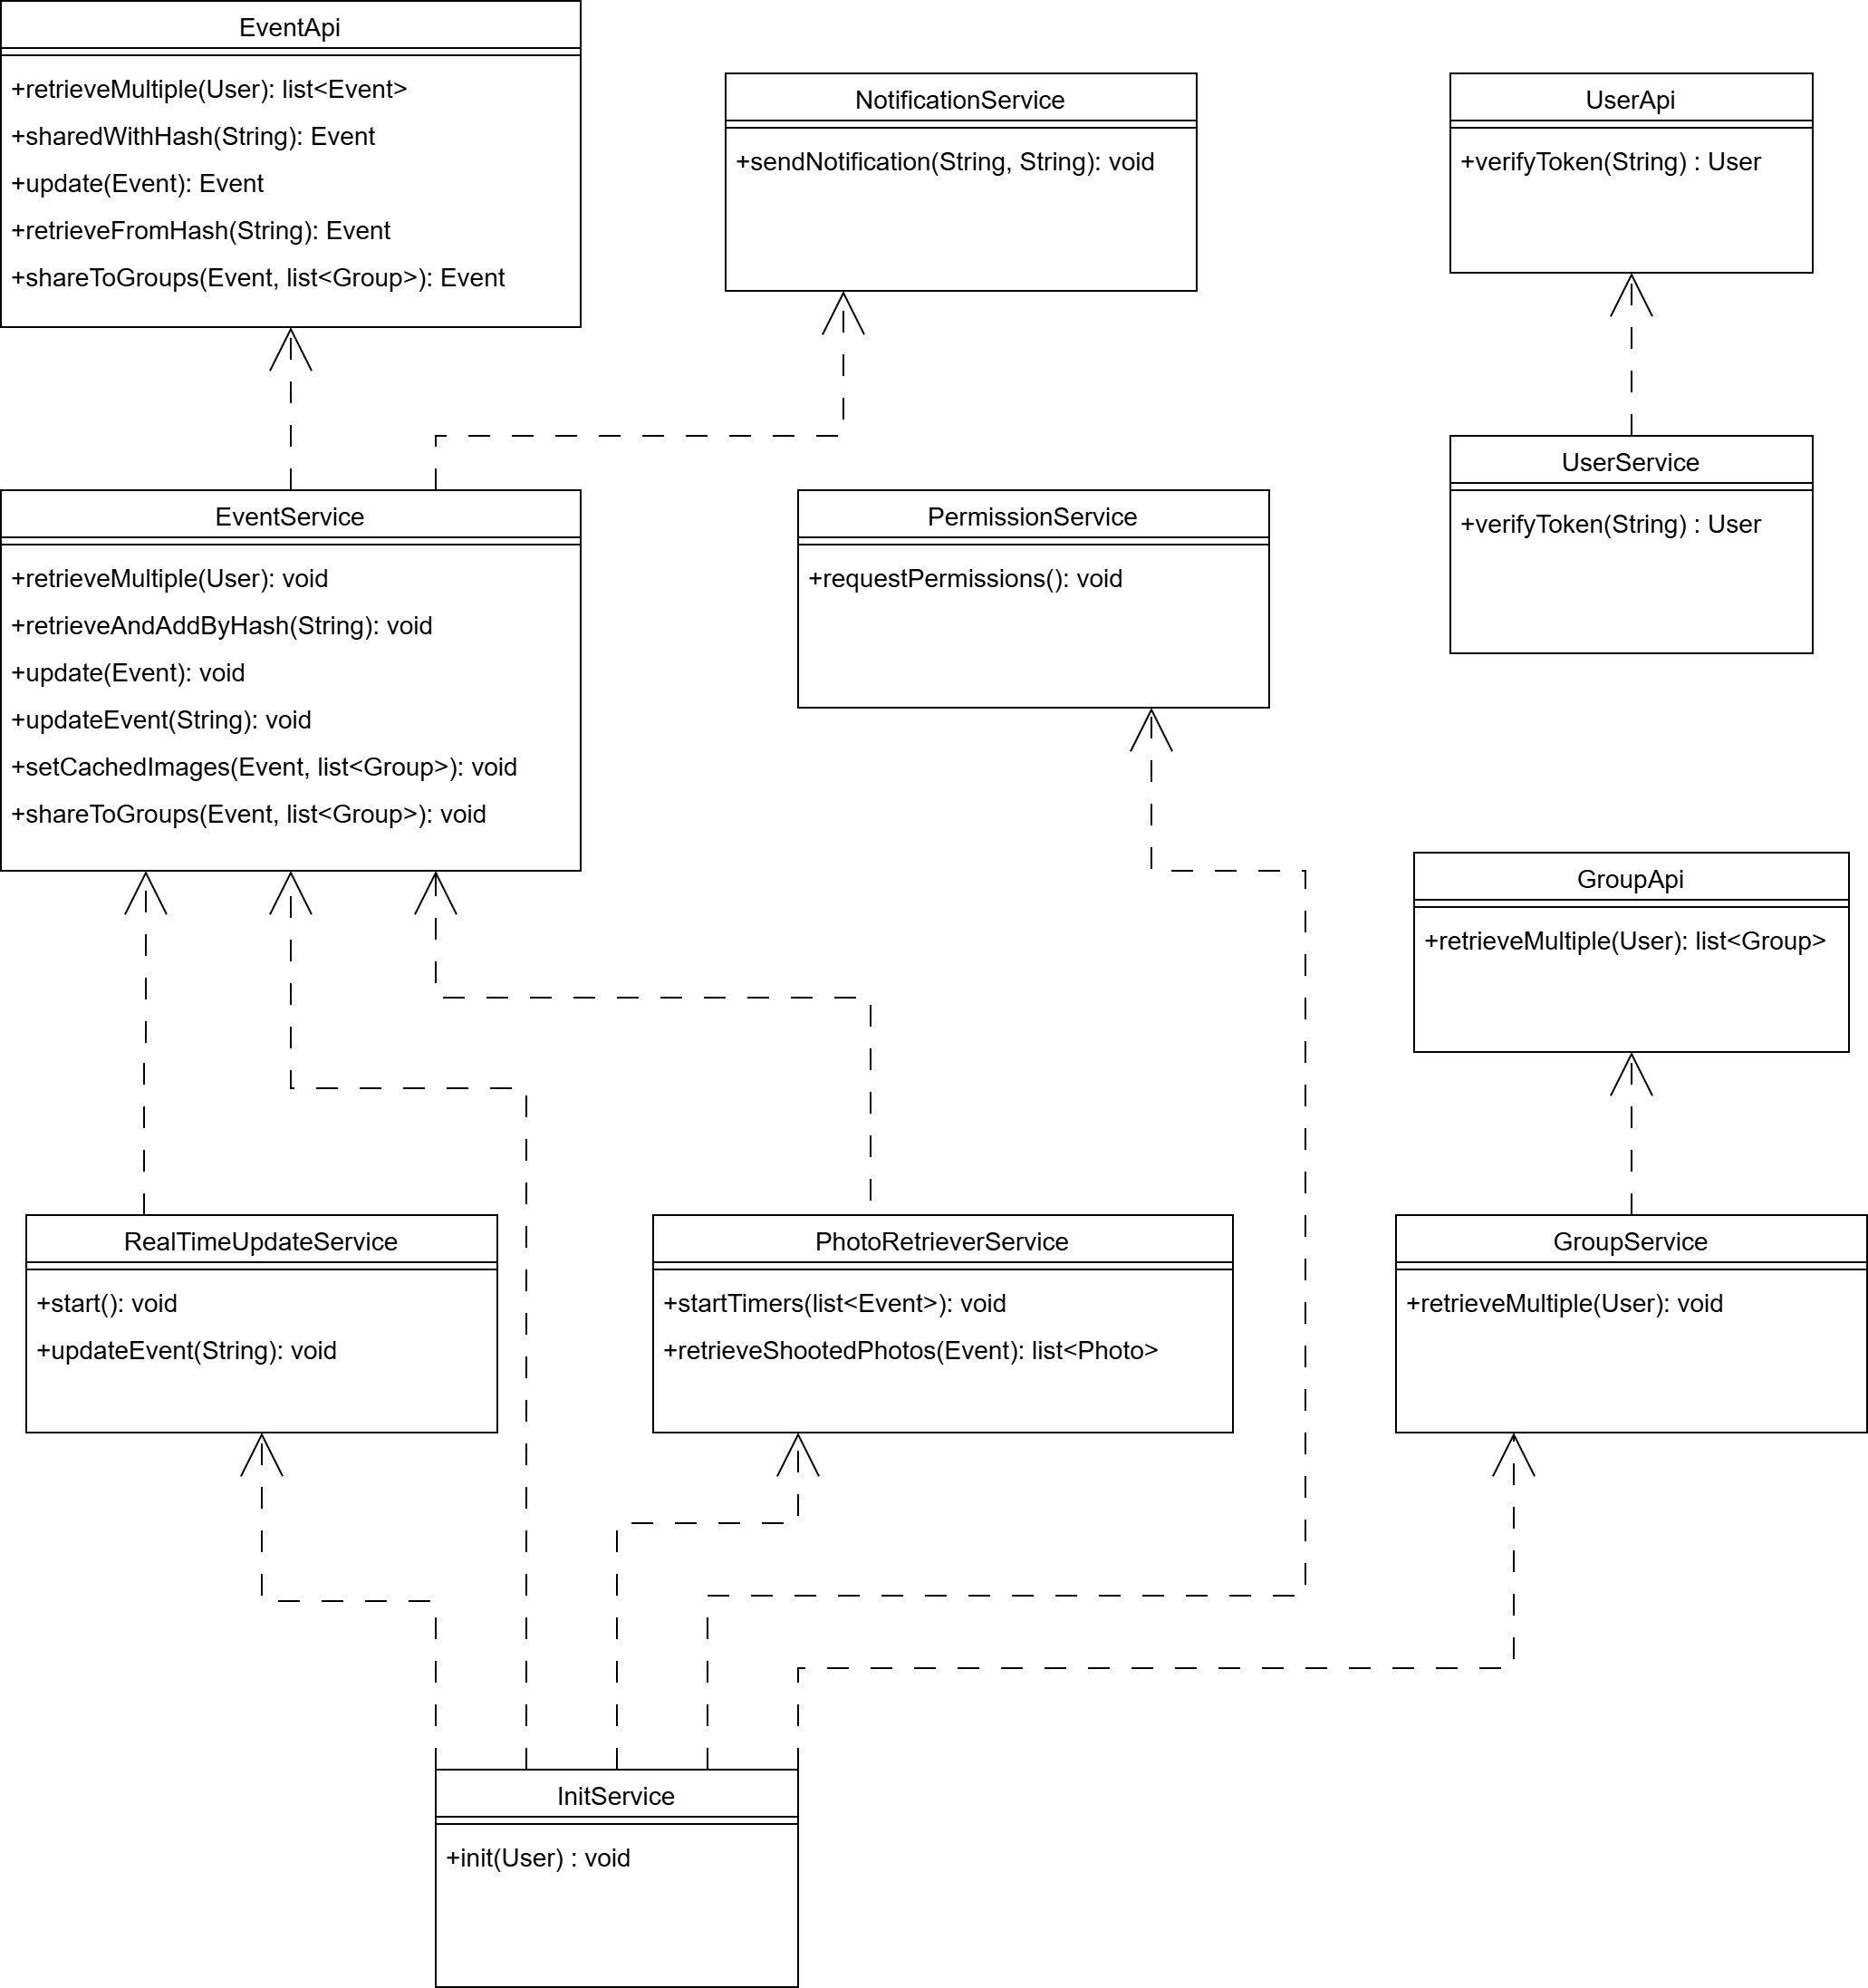
\includegraphics[width=\textwidth]{FrontServiceClassDiagram.png}
        \caption{Modello delle classi del client}
    \end{center}
\end{figure}

Non tutte le funzionalità sono però correlate direttamente al dominio.
Per questo motivo si creano servizi ausiliari dedicati, 
anch'essi separatati in base al ruolo che ricoprono.
\clearpage
Un servizio è stato dedicato all'acquisizione e al salvataggio dei permessi necessari per operare, 
quali l'invio delle notifiche e l'accesso alla galleria. 
Mette a disposizione degli altri processi, quindi, la conferma dell'accesso ai permessi richiesti o, 
in caso non lo si possegga, gestirà il suo ottenimento.\\ 
\\
L'invio delle notifiche e la ricezione degli aggiornamenti, 
per quanto concettualemte simili e strettamente correlati,
sono stati implementati in due componenti differenti. 
Le notifiche possono essere infatti richieste anche da altri metodi, 
e ad ogni aggiornamento potrebbe non corrispondere una notifica.
La ricezione delle modifiche in tempo reale avviene usando il pattern observer, 
nel quale il servizio si connette ad un canale e rimane in attesa di eventuali messaggi.

\begin{figure}[h!]
    \begin{center}
        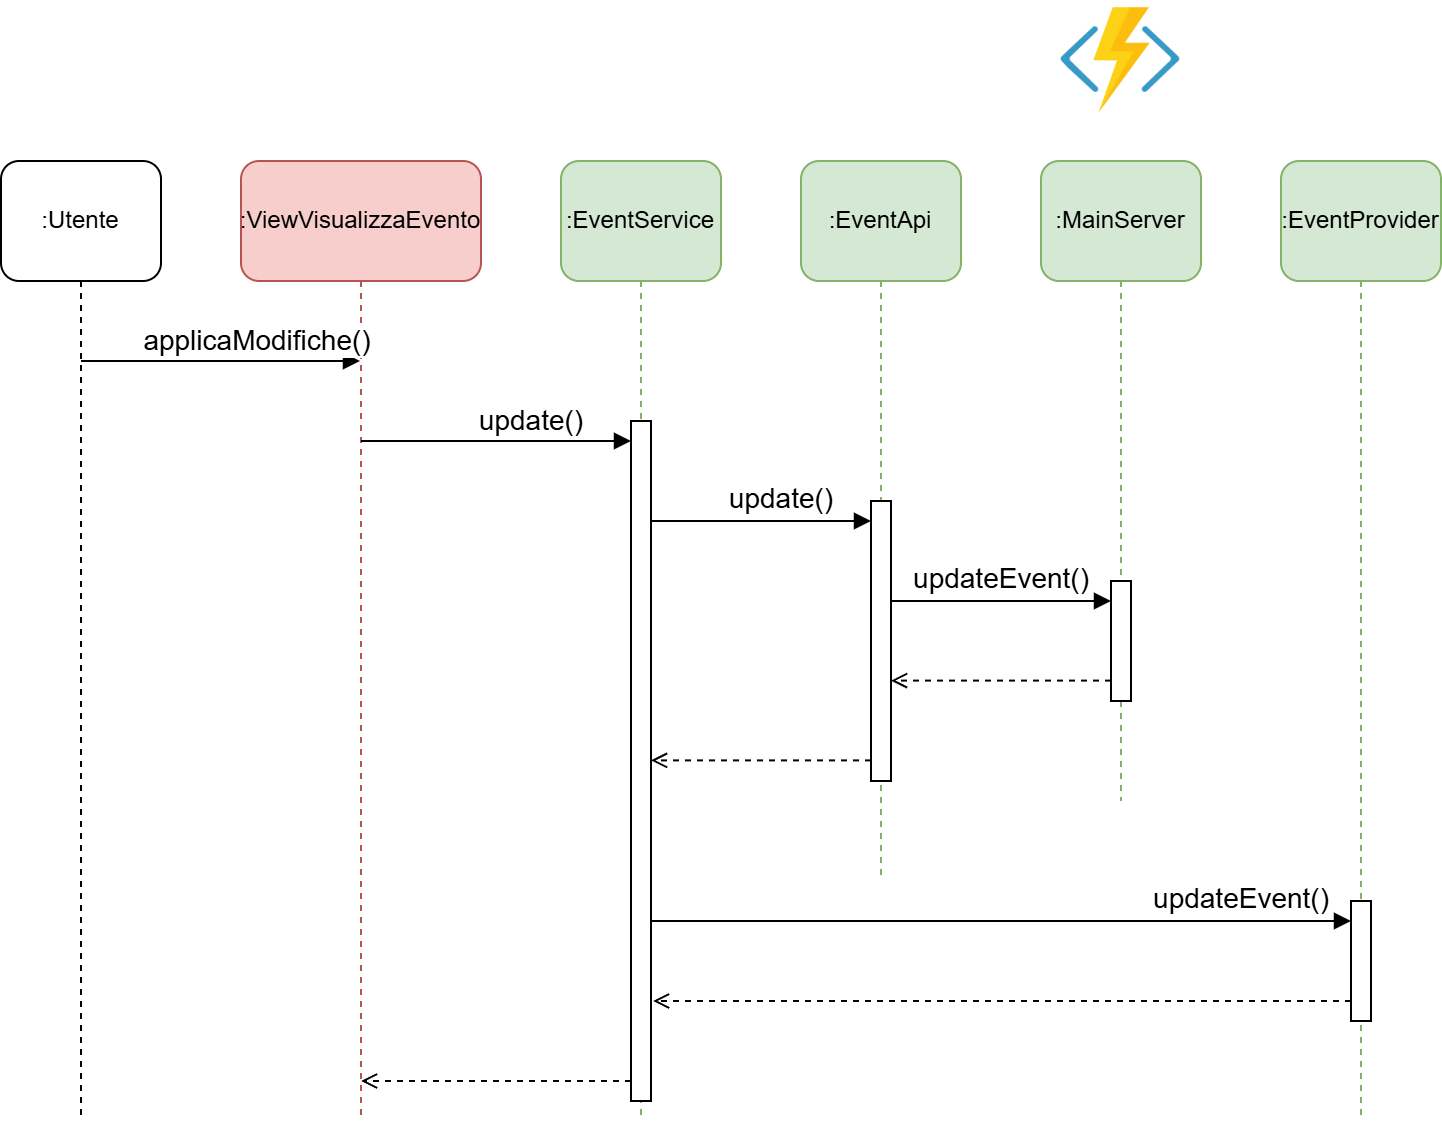
\includegraphics[width=\textwidth]{IIModificaEvento1.png}
        \caption{Diagramma di sequenza della modifica di un evento}
    \end{center}
\end{figure}

\clearpage

Il salvataggio in memoria locale dei dati risulta fondamentale per la reattività dell'applicazione,
in quanto permette di ridurre le richieste di dati e velocizza il loro recupero.
La memoria locale viene implementata grazie a classi Provider, create in relazione agli elementi del dominio.
Un'altra funzionalità centrale dell'applicazione è il recupero automatico 
delle foto scattate durante l'evento. 
Questo richiede la pianificazione di azioni automatiche nel tempo,
così come la scansione della galleria per trovare le immagini interessate.
Sia la gestione locale della memoria che il recupero delle immagini vedono uno o più componenti dedicati.
La loro realizzazione viene trattata nei capitoli seguenti.\\
\\
Durante l'implementazione della logica applicativa si sono dovuti affrontare altri problemi quali, degni di nota, 
la gestione della condivisione di un evento tramite link e l'inizializzazione dell'applicazione.\\

\begin{figure}[h!]
    \begin{center}
        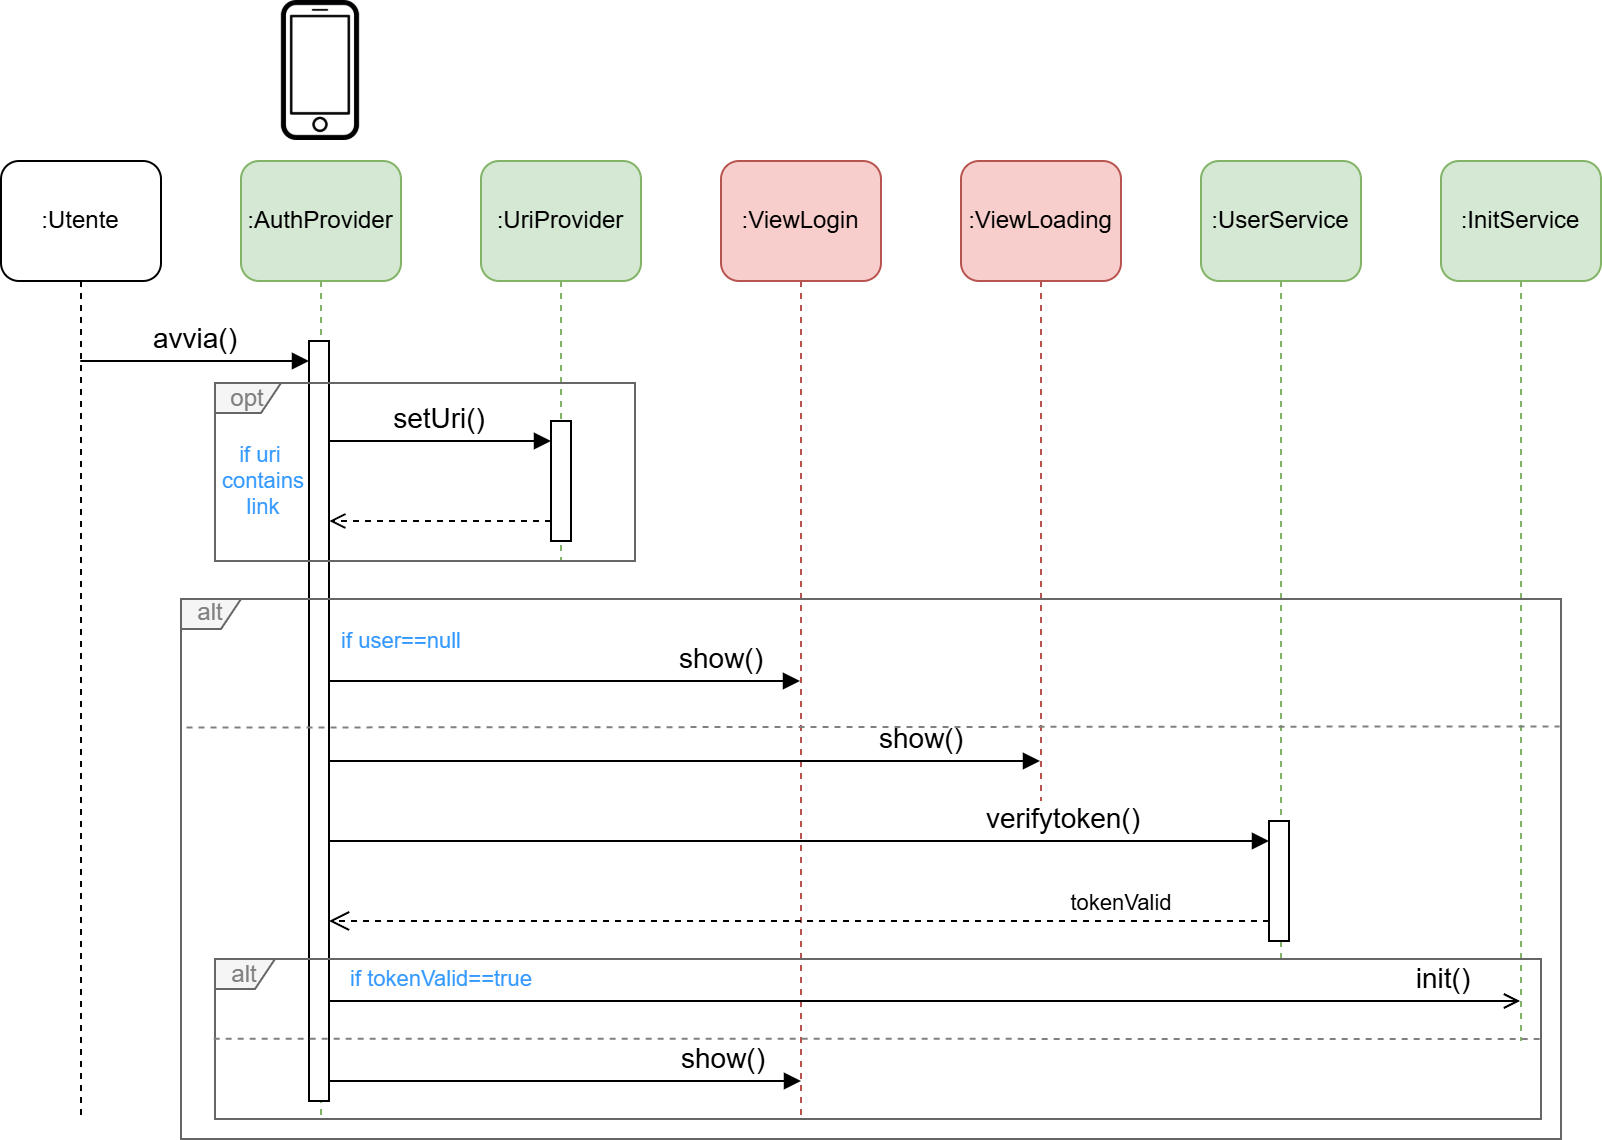
\includegraphics[width=\textwidth]{Avvio.png}
        \caption{Diagramma di sequenza dell'avvio dell'applicazione}
    \end{center}
\end{figure}

La condivisione di un evento tramite link consiste in due passaggi principali: 
la creazione del link stesso e il sucessivo ritrovamento dell'evento associato.
La generazione del link avviene tramite l'unione del dominio del server con il codice identificativo dell'evento.
\clearpage
All'apertura dell'applicazione tramite link viene estratto il codice identificativo dell'evento 
per la sucessiva richiesta dei dati al server.
Se l'utente non si è ancora autenticato, però, il router dell'applicazione lo reindirizza alla schermata di login, 
cambiando il link e perdendo l'informazione allegata.
Per evitare questo problema, nel momento in cui l'utente accede all'applicazione tramite un link,
le sue informazioni vengono salvate in memoria locale.
Al termine del login, se sono presenti dati salvati, l'utente verrà indirizzato alla schermata degli eventi proposti, 
che recupererà i dati relativi all'evento, per poi mostrarli a video.

\begin{figure}[h!]
    \begin{center}
        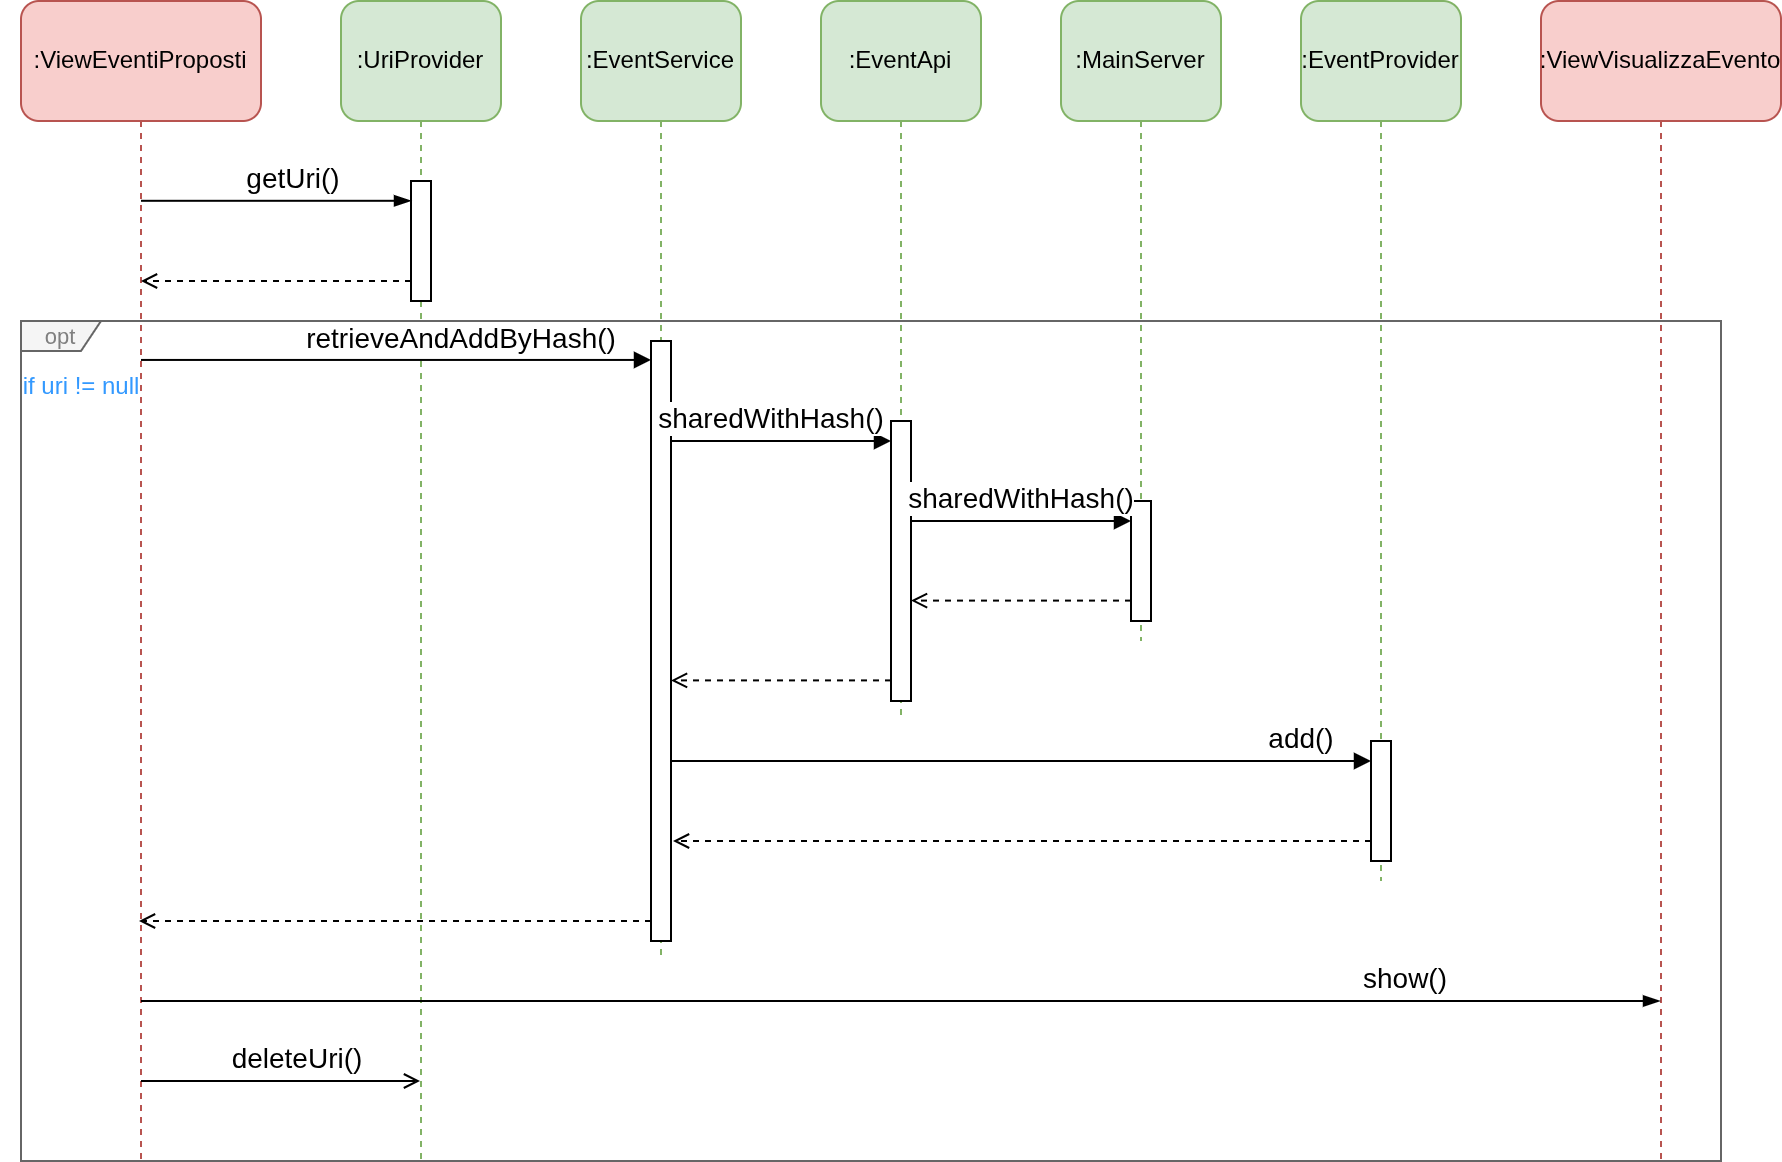
\includegraphics[width=\textwidth]{IIVisualizzaEventiProposti.png}
        \caption{Diagramma di sequenza della visualizzazione degli eventi proposti}
    \end{center}
\end{figure}

\clearpage

La fase di inizializzazione avviene a seguito di un login andato a buon fine.
Parallelamente alla visualizzazione della schermata iniziale si recuperano i dati 
relativi ai profili associati all'utente e vengono fatti partire i servizi autonomi. 
In particolare, vengono controllati i permessi necessari per i quali, se non ancora concessi, 
verrà richiesto l'ottenimento. 
Viene inoltre avviato il servizio di ricezione degli aggiornamenti, che si connette al canale relativo all'utente.
Per ogni profilo vengono, sempre in maniera parallela, recuperati i gruppi e gli eventi associati.
Al termine della ricezione degli eventi, indipendentemente dalle altre richieste, 
per ogni evento sucessivo al momento attuale viene avviato un timer, che scatena, 
al momento giusto, il recupero delle immagini.
Se l'applicazione è stata aperta tramite link di condivisione, 
la schermata a cui si verrà reindirizzati sarà quella degli eventi proposti, altrimenti quella degli eventi confermati.\\
\\

\begin{figure}[h!]
    \begin{center}
        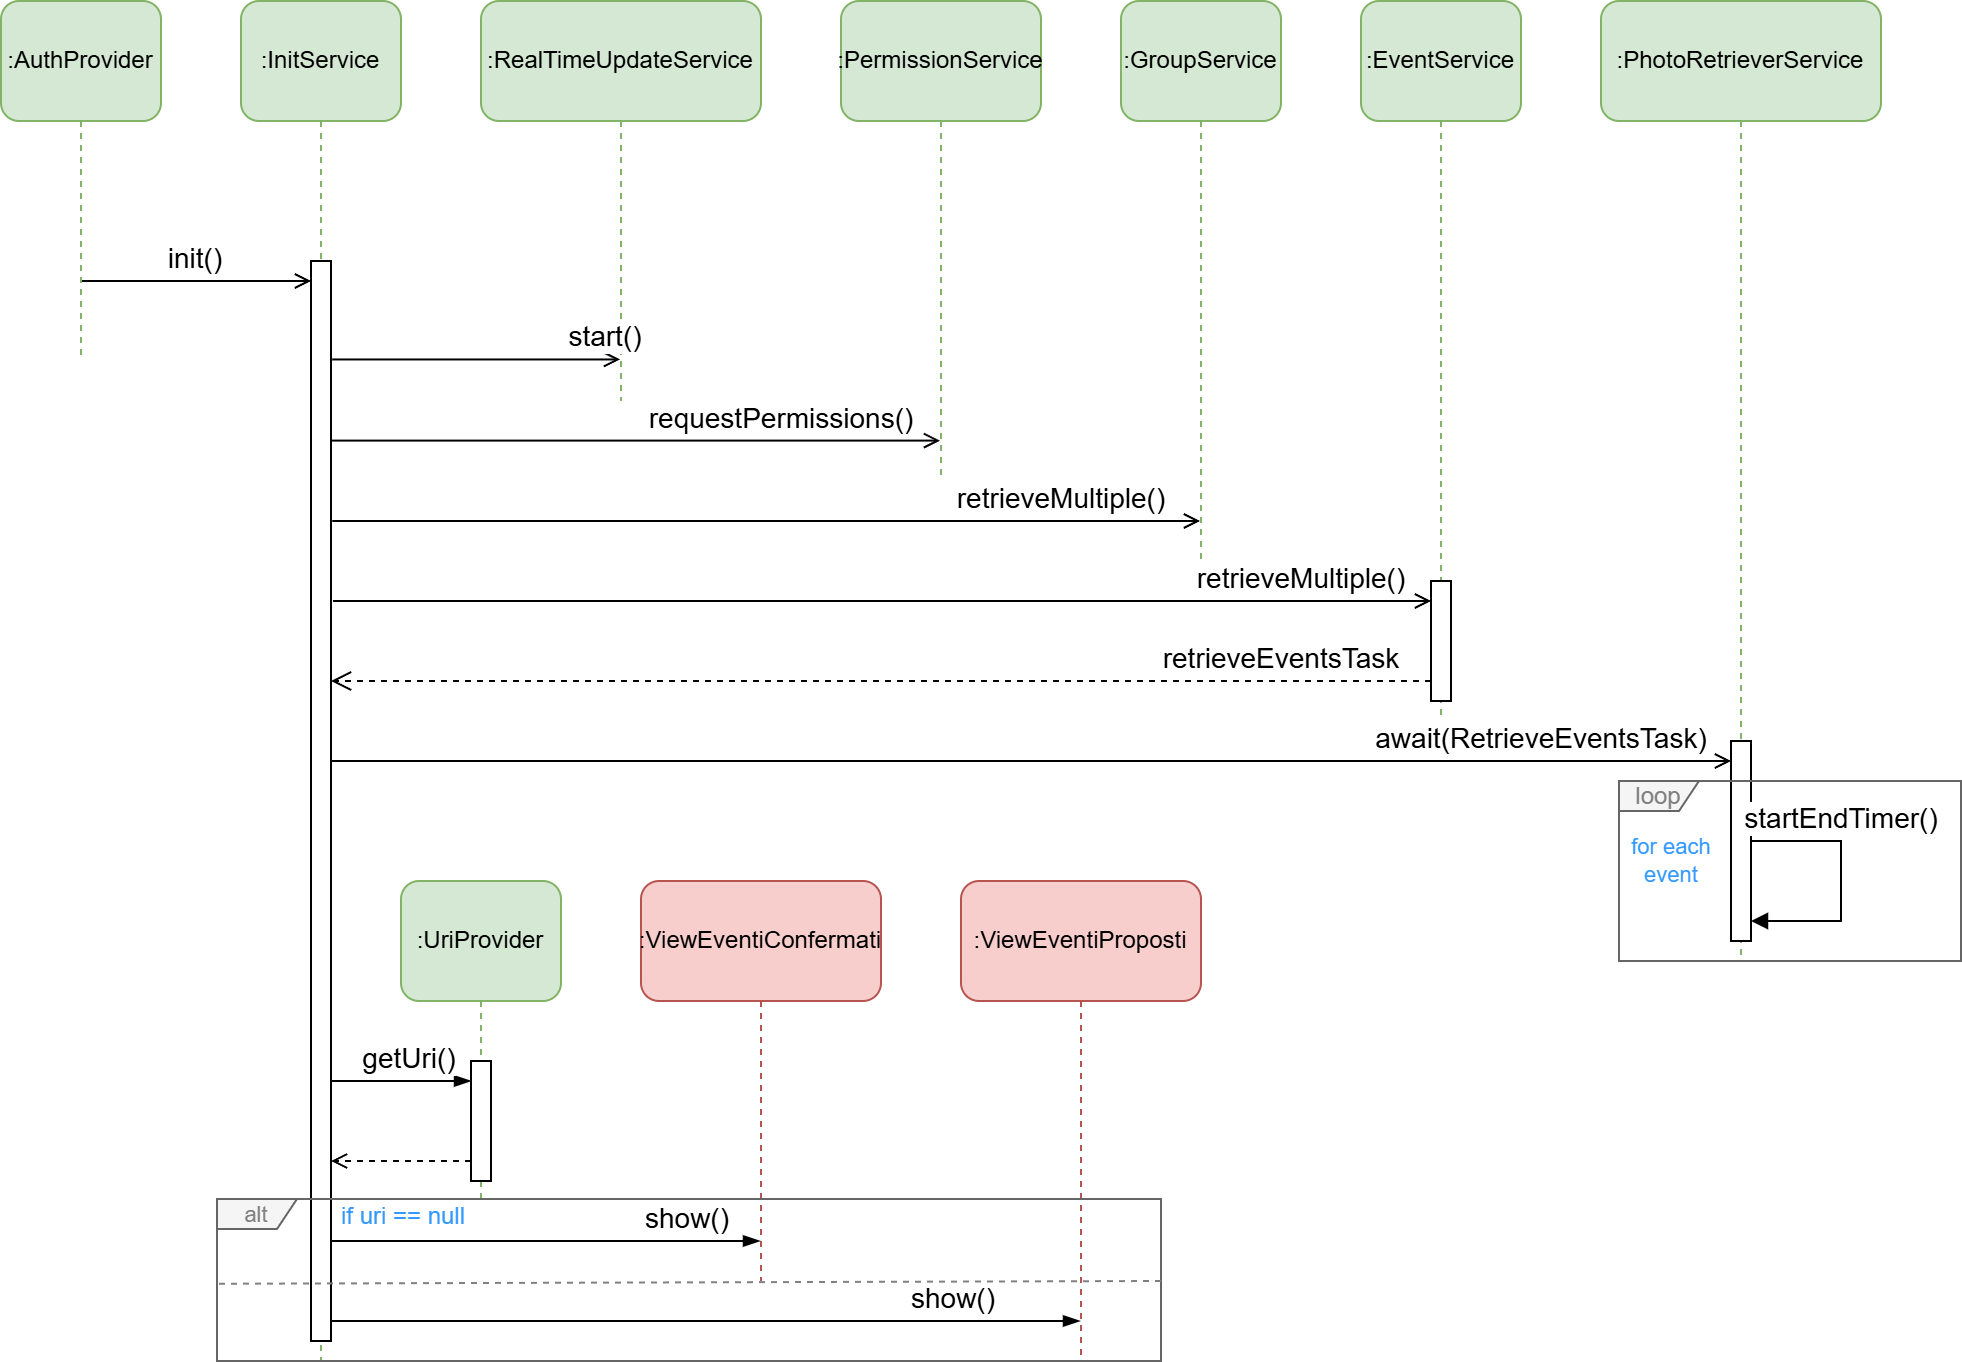
\includegraphics[width=\textwidth]{Init.png}
        \caption{Diagramma di sequenza della fase di inizializzazione }
    \end{center}
\end{figure}


\clearpage

\subsubsection{La distribuzione}

Per quanto Flutter consenta di uniformare l'esperienza utente su dispositivi diversi e semplifichi la compilazione per le varie piattaforme,
alcune configurazioni rimangono comunque dipendenti dalla tecnologia su cui l'applicazione viene eseguita.
Di conseguenza, ciascun eseguibile richiede una manutenzione aggiuntiva, inclusi gli aggiornamenti delle dipendenze specifiche,
sia a livello di deployment che di gestione delle versioni.\\
\\
In una fase iniziale dello sviluppo, nell'ottica di coprire il più ampio mercato possibile con il minor numero di piattaforme,
si è deciso di sviluppare una versione fruibile via web e una per dispositivi Android.\\
\\
Nell'ambito delle tecnologie offerte da Azure per la  distribuzione del codice web, si è scelto Azure Static Web App, un servizio di hosting progettato per applicazioni web statiche. \\
\\
La preferenza per questa soluzione è derivata dalla affidabilità dell'infrastruttura di Azure e dai bassi costi operativi per un utilizzo limitato,
fattori che la rendono particolarmente vantaggiosa.\\
\\
Questa selezione è stata resa possibile in quanto l’interfaccia sviluppata non prevede la creazione dinamica di contenuti,
ovvero la pagina che viene restituita rimane invariata indipendentemente dall’utente che effettua la richiesta.
I dati specifici dell’utente verranno infatti richiesti ad un server terzo (qualora non siano già presenti in una cache locale).
Questa scelta consente di rendere l’interfaccia grafica completamente indipendente dall’identità dell’utente,
migliorando così le prestazioni e riducendo il carico computazionale delegato a Azure Static Web App.\\
\\
Inoltre, in attesa della pubblicazione dell’applicazione sull’App Store di Android, l’eseguibile è stato temporaneamente reso disponibile tramite Azure Storage Container.
Questo servizio consente l’archiviazione e la distribuzione di file di varie tipologie, fornendo un link diretto per il recupero.
\clearpage
\begin{figure}[h!]
    \begin{center}
        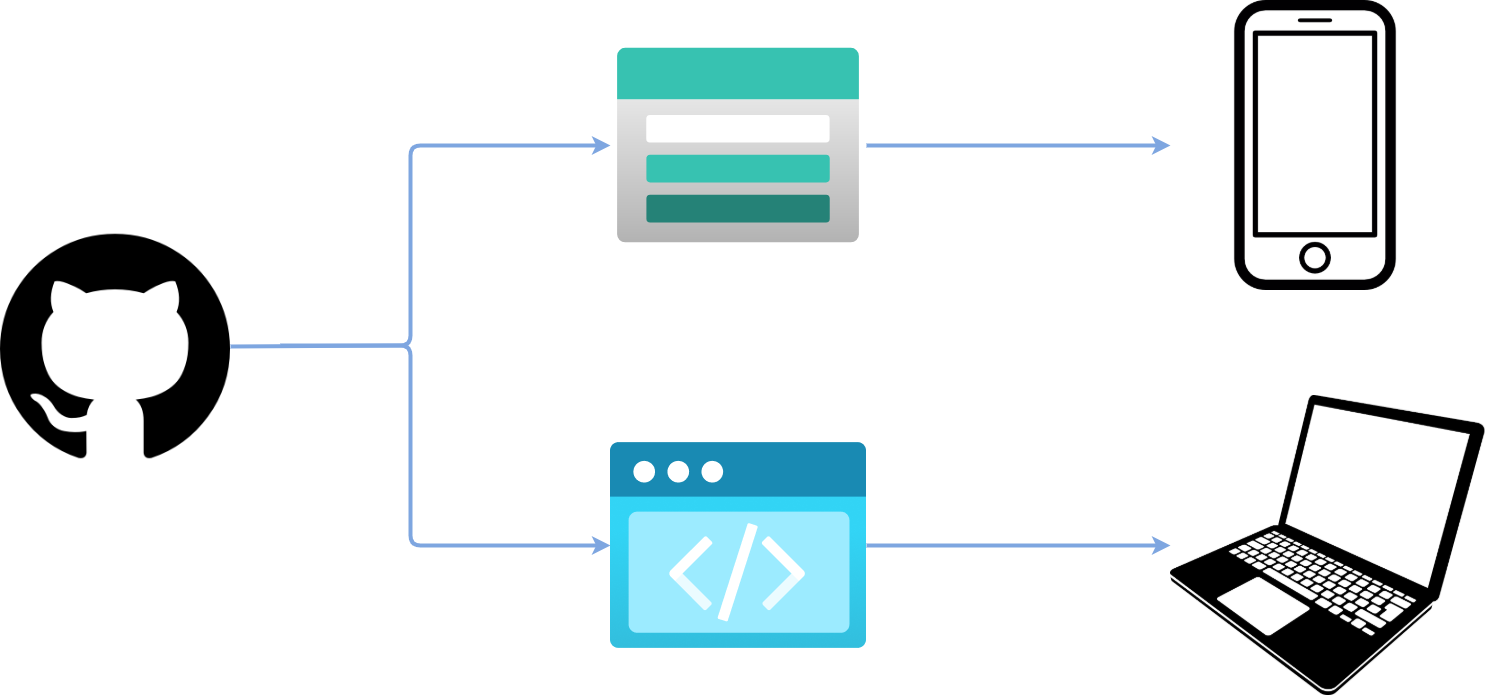
\includegraphics[height=0.28\textheight]{DeployFront.png}
        \caption{Diagramma di aggiornamento e distribuzione del client}
    \end{center}
\end{figure}

\subsubsection{L'aggiornamento}
Per garantire un processo di aggiornamento efficiente e automatizzato,
sia il codice distribuito sulla web app che l’applicativo ospitato nel container vengono gestiti tramite GitHub Actions,
che ne assicura l’aggiornamento automatico a ogni nuova versione. \\
\\

Nella fruizione tramite browser, il codice si aggiorna automaticamente a ogni accesso, mentre per l’applicativo su dispositivo mobile è necessaria una reinstallazione manuale.
Per questa ragione, gli utenti dell’applicazione verranno notificati tempestivamente ogni volta che sarà disponibile una nuova versione.\\
\\
\clearpage








\subsection{L’architettura del server principale}

Per poter essere in grado di gestire un numero elevato di richieste in tempi ridotti, l’applicazione deve garantire un’elevata scalabilità.\\
\\
Capace di soddisfare al meglio questa esigenza è Azure Functions, un servizio serverless che consente di suddividere il codice in unità indipendenti,
ciascuna eseguita in un ambiente di esecuzione unico per ogni richiesta.
Questa caratteristica, combinata con la virtualizzazione dell’ambiente di esecuzione offerta dal cloud, consente una scalabilità potenzialmente illimitata.\\
\\
L’indipendenza e la natura stateless di ogni funzione, ovvero la sua esecuzione svincolata dalle informazioni sullo stato o sulla sessione, sono responsabilità dello sviluppatore.
Ogni funzione segue il principio di singola responsabilità, eseguendo un unico compito specifico.
Tuttavia, nel caso di richieste che necessitino l’esecuzione coordinata di più funzioni, Azure Durable Functions fornisce una soluzione efficace.\\
\\
Integrata all’interno delle Azure Functions, Azure Durable Function consente la creazione di una funzione orchestrator,
incaricata di gestisce l’ordine, lo stato, il ciclo di vita e le risposte delle varie funzioni coinvolte nell’elaborazione della richiesta.\\
\\
Mantenendo un'architettura indipendente e scalabile, questa soluzione consente di gestire efficacemente scenari in cui un’esecuzione sequenziale delle operazioni è cruciale,
dove è necessario effettuare tentativi aggiuntivi in caso di errore o fallimento o si richiede l'attesa del completamento di operazioni con un tempo di esecuzione prolungato.\\
\\
Tuttavia, l'architettura stateless e l’accoppiamento debole tra orchestrator e funzioni in esecuzione causano un tempo di risposta delle Azure Durable Functions più elevato.
Per ottimizzare l’allocazione delle risorse, il sistema avvia perciò solo le funzioni strettamente necessarie all’esecuzione del compito determinato,
stanziando al minimo il consumo computazionale.\\
\\

\subsubsection{La scelta del linguaggio}
Come linguaggio di programmazione per lo sviluppo delle funzioni è stato utilizzato C\#.
La consapevolezza che sia l’ambiente di sviluppo di C\#, ovvero il framework .Net, sia la piattaforma Azure siano entrambi sviluppati e mantenuti dalla stessa azienda, Microsoft,
garantisce elevati livelli di stabilità, supporto e coordinamento delle tecnologie adottate.\\
\\
L’integrazione con Entity Framework Core permette la mappatura direttamente in oggetti dei componenti del dominio, 
semplificando così la logica delle relazioni e astraendo le comunicazioni con il database.
Grazie all’utilizzo delle proprietà virtuali degli oggetti si può applicare il lazy loading, 
riducendo il numero di richieste al database solo a quando esse sono strettamente necessarie, mantenendo in codice a livello logico ed ottimizzandone le prestazioni.
\subsubsection{Lo sviluppo}
Lo sviluppo è stato condotto utilizzando Visual Studio Code, piattaforma che, grazie ad apposite estensioni,
consente un collegamento diretto ai servizi cloud Azure, semplificando il processo di aggiornamento del codice, rendendolo estremamente lineare ed immediato.\\
\\
Azure Function in ambiente .Net supporta due modelli di esecuzione e sviluppo: in-process worker o isolated worker.
Il worker è il processo all’interno dell’applicativo che gestisce la creazione delle risorse e l’esecuzione delle funzioni in risposta alle richieste.
Nella modalità in-process, la funzione viene eseguita all’interno dello stesso processo del worker che l’ha generata,
riducendo la quantità di allocazione delle risorse necessarie ma condividendo l’ambiente di esecuzione.
Nel modello isolated, invece, ogni funzione viene eseguita attraverso un processo indipendente dedicato,
garantendo maggiore isolamento e quindi riducendo le possibili dipendenze tra le funzioni. \\
\\
Inoltre, il modello isolated worker offre ulteriori vantaggi, grazie al maggiore supporto fornito:
innanzitutto esso prevede una maggiore compatibilità, grazie al più ampio numero di versioni del framework .Net,
a differenza del modello in-process, limitato alle sole versioni con supporto a lungo termine.
In secondo luogo, il supporto per la creazione di middleware personalizzati 
permette l’elaborazione di un codice intermedio tra la chiamata e l’esecuzione della funzione,
funzionalità invece non disponibile nel modello in process.
Considerati questi vantaggi, le funzioni sono state sviluppate utilizzando il modello isolated worker 
per garantire maggiore flessibilità, compatibilità e modularità dell’architettura.
\clearpage
\subsubsection{TODO Titolo da trovare}



\begin{figure}[h!]
    \begin{center}
        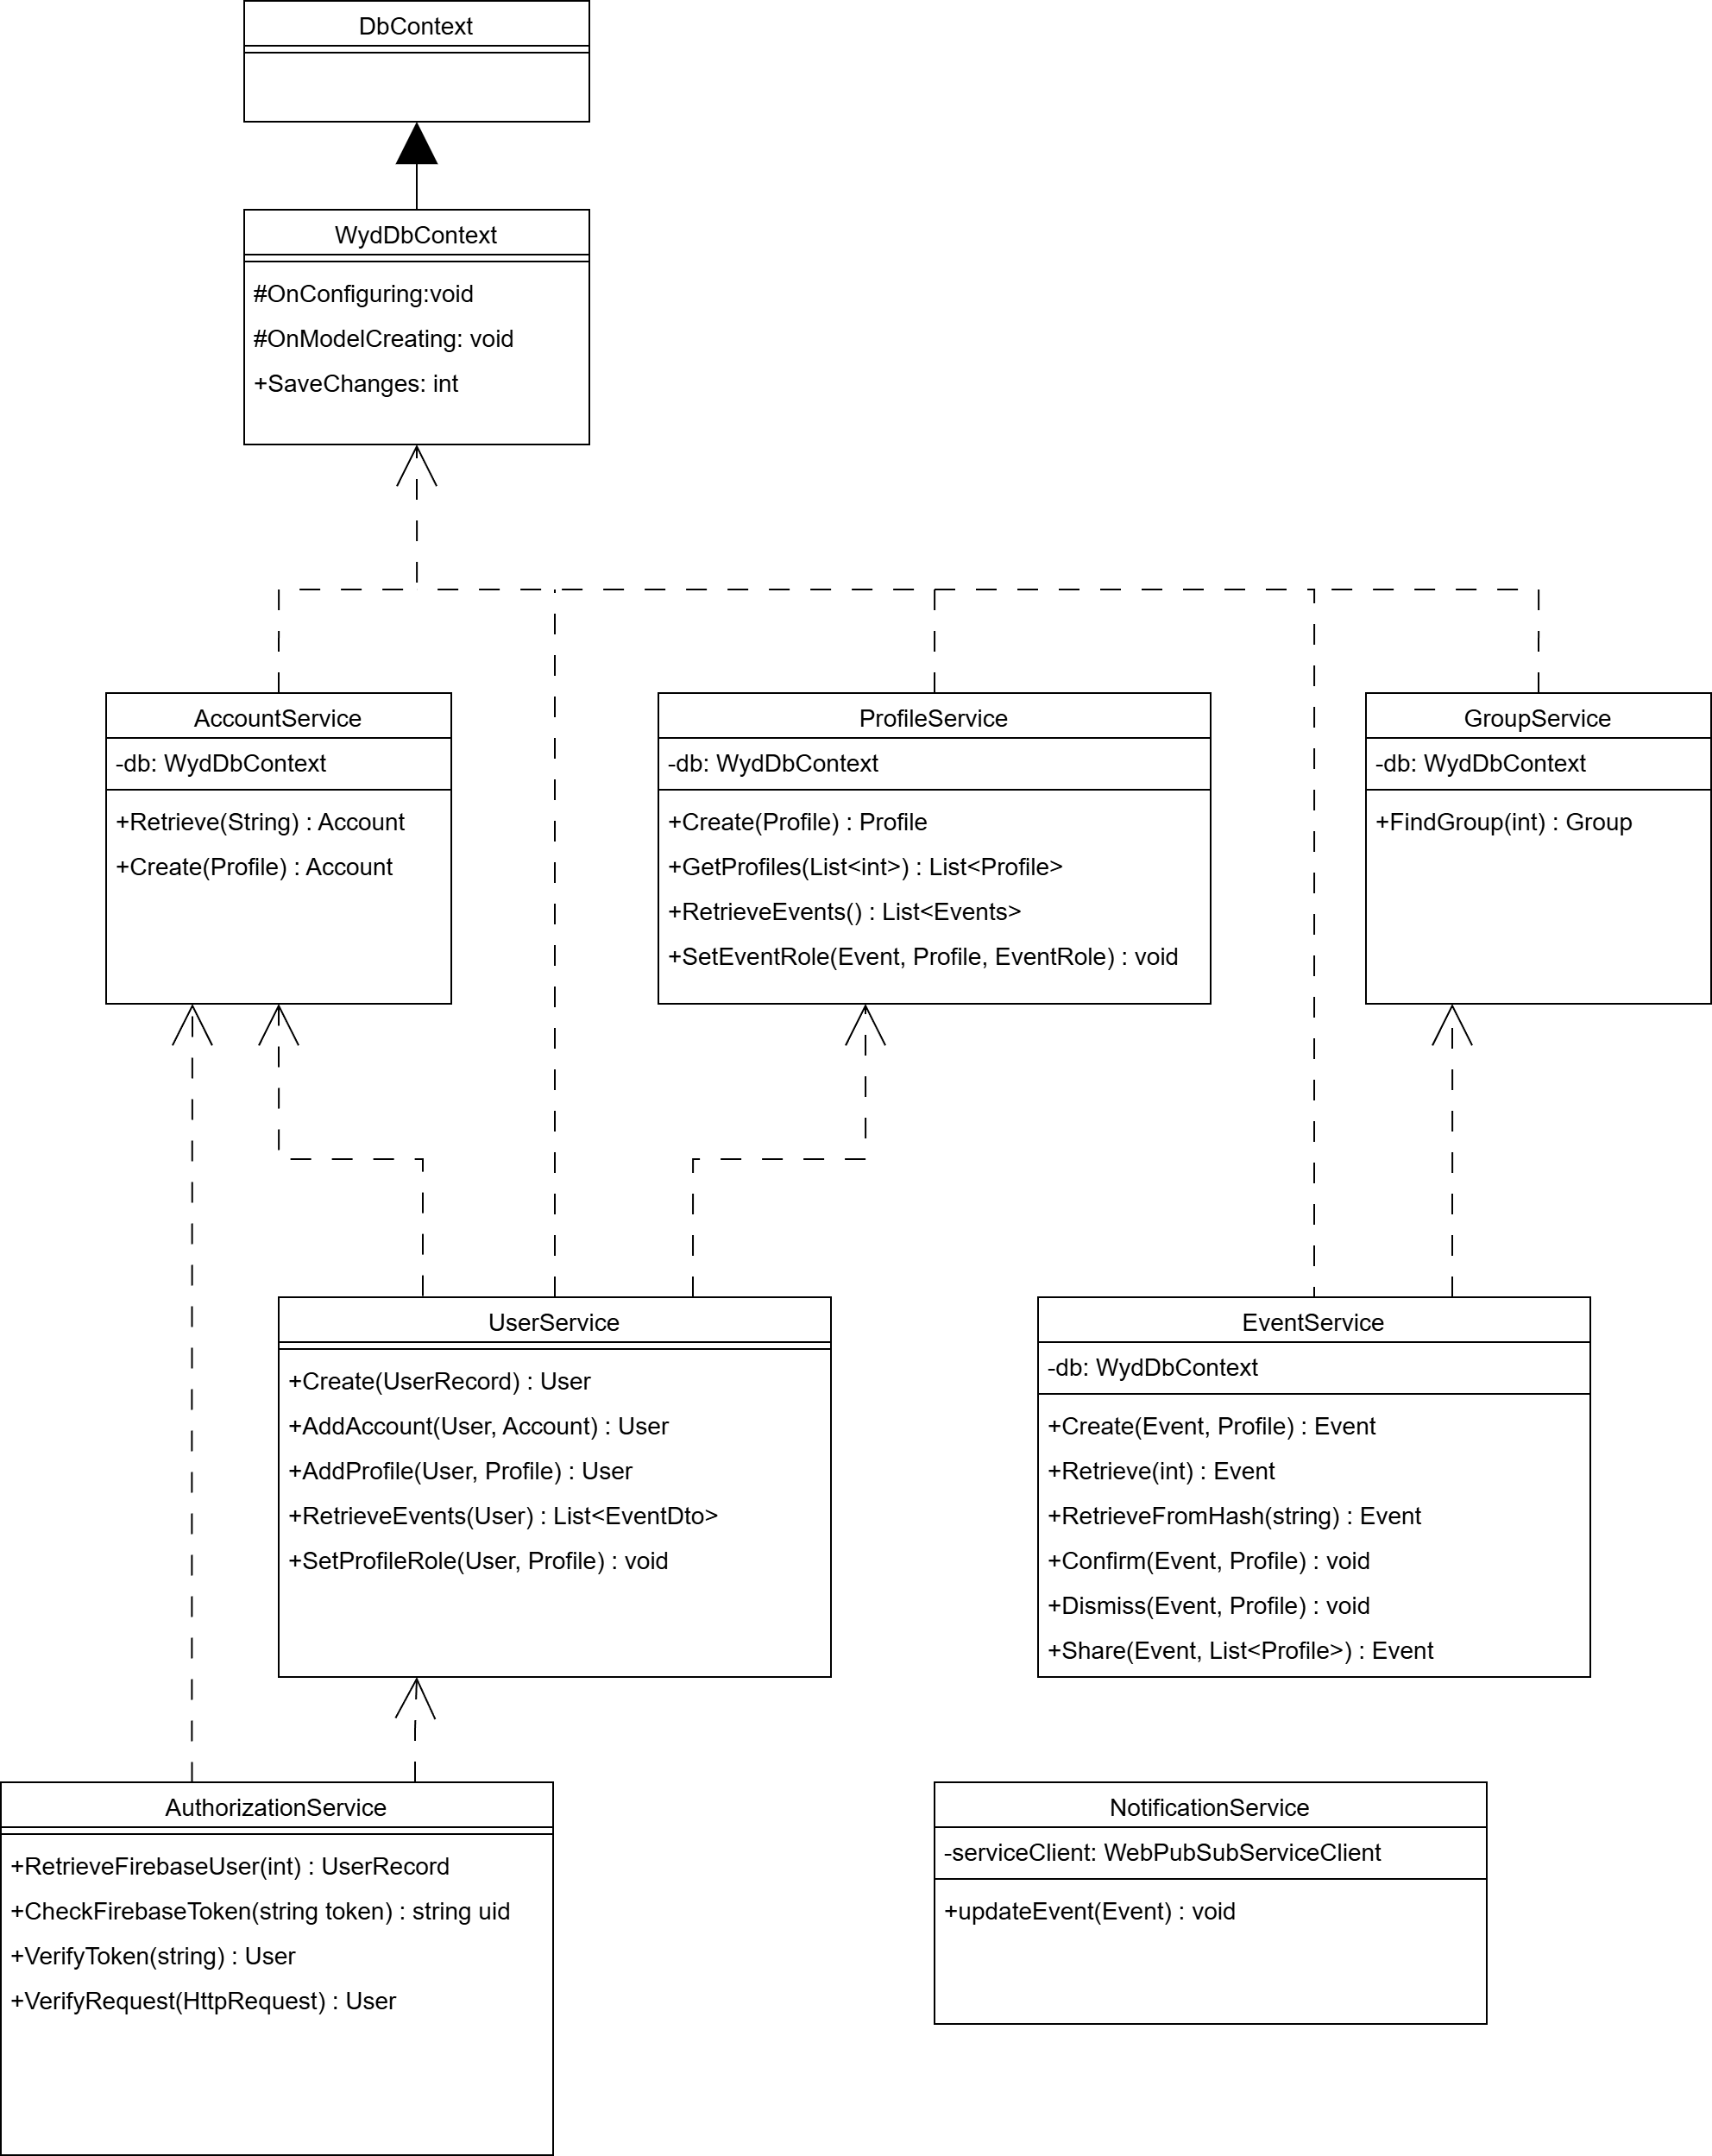
\includegraphics[width=\textwidth]{ServiceClassDiagram.png}
        \caption{Modello delle classi del client}
    \end{center}
\end{figure}

\begin{figure}[h!]
    \begin{center}
        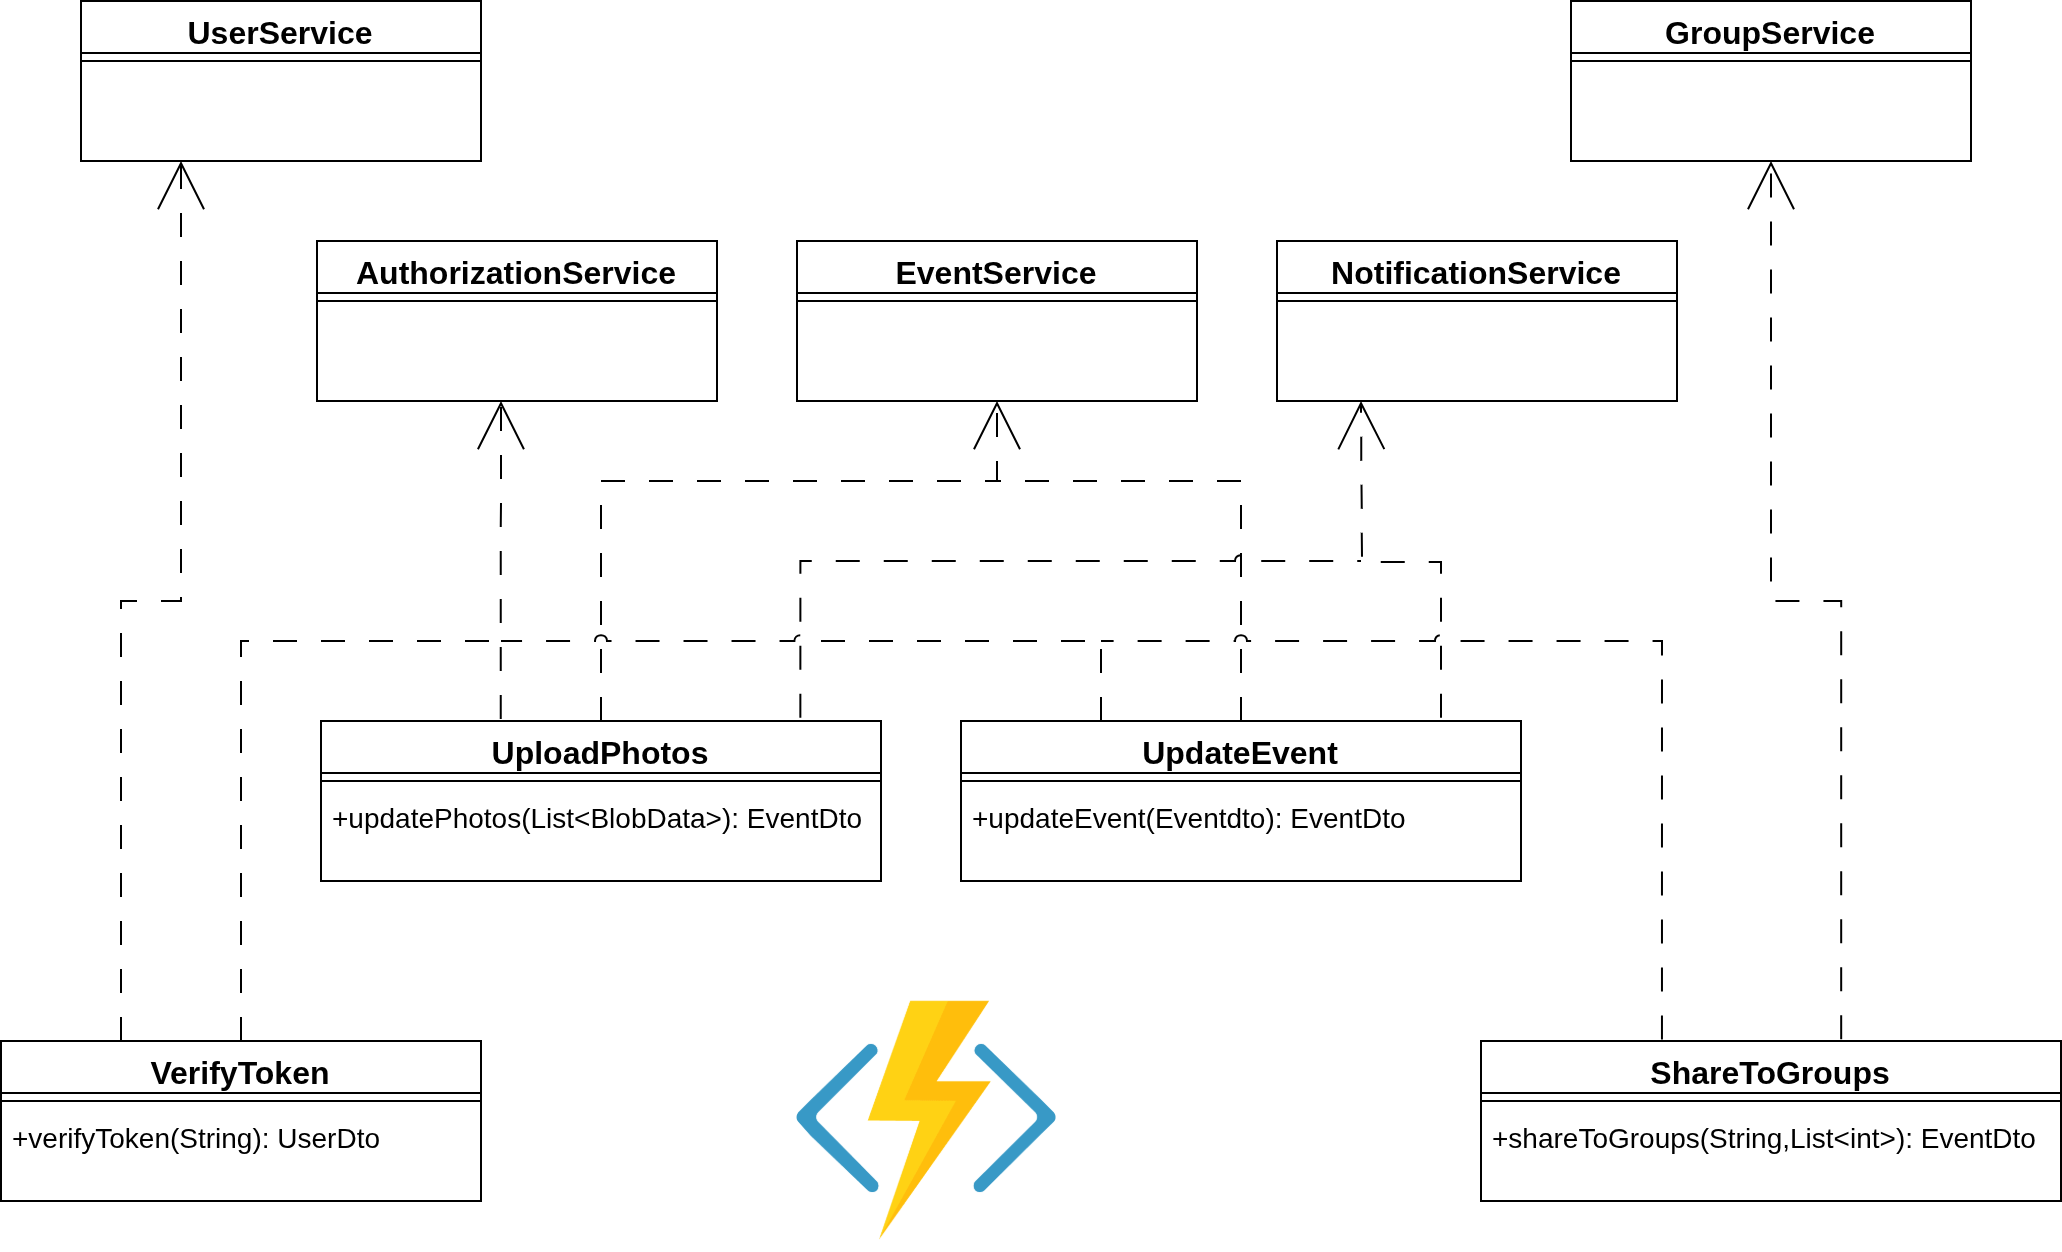
\includegraphics[width=\textwidth]{FunctionClassDiagram.png}
        \caption{Modello delle classi del client}
    \end{center}
\end{figure}

\begin{figure}[h!]
    \begin{center}
        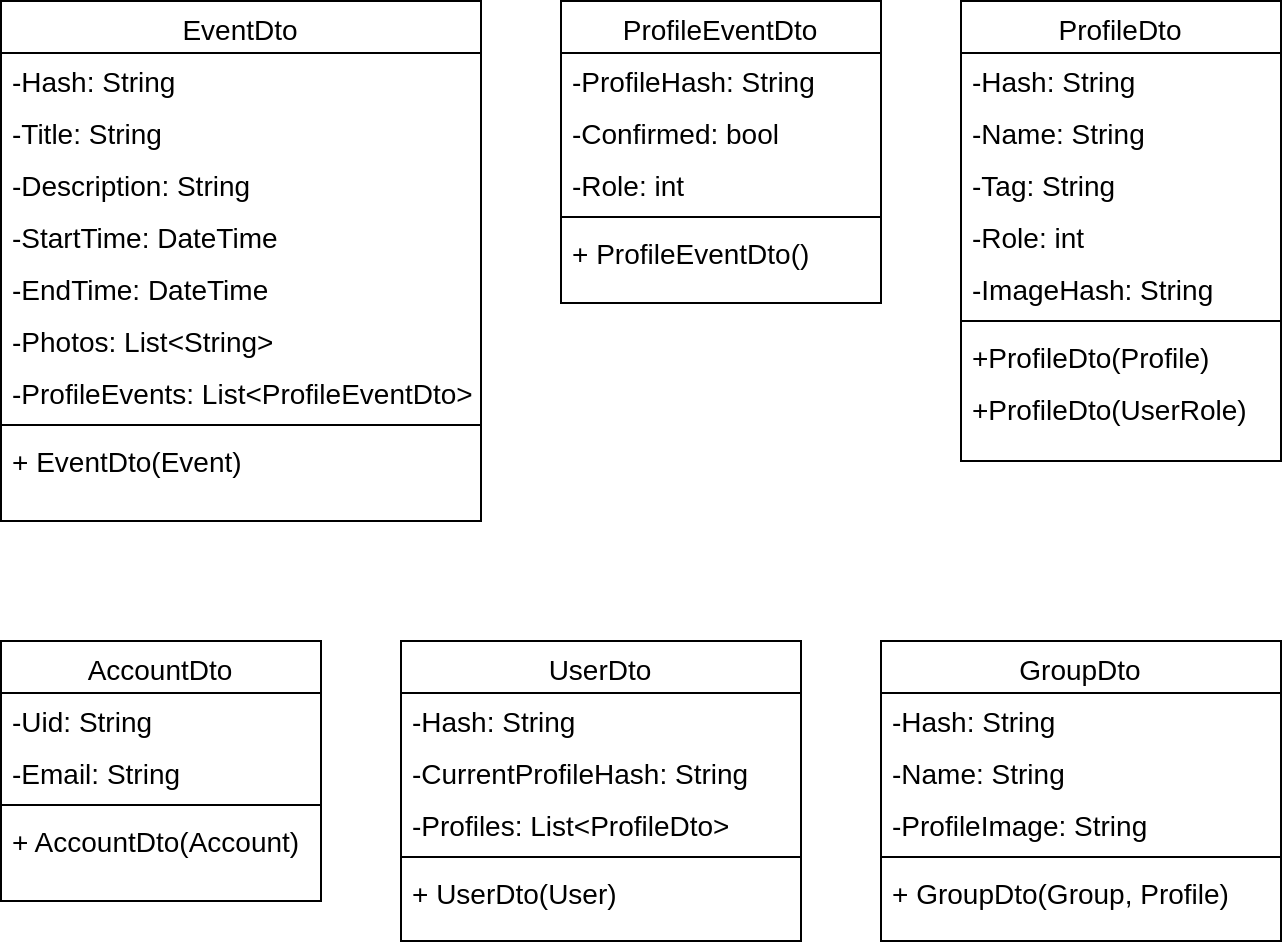
\includegraphics[width=\textwidth]{DTOClassDiagram.png}
        \caption{Modello delle classi del client}
    \end{center}
\end{figure}
\clearpage




\subsection{Autenticazione}


Poiché la modalità di autenticazione rappresenta un elemento cruciale per l’esperienza dell’utente, 
in quanto deve assicurare un accesso sicuro all’applicazione mantenendone la semplicità, la facilità del processo autenticazione deve essere garantita.
Offrire agli utenti la possibilità di autenticarsi tramite il proprio authentication provider di fiducia migliora sicuramente l’usabilità e l’apprezzamento degli utenti, 
ma è altrettanto essenziale consentire la possibilità di creare account dedicati esclusivamente all’applicazione.
Di conseguenza, il sistema di gestione degli accessi deve supportare sia la registrazione e la gestione autonoma degli account specifici per il servizio, 
sia fornire l'integrazione con provider di autenticazione esterni.\\
\\
Per lo scopo, Azure fornisce Microsoft Entra ID, parte della suite di servizi di autenticazione e autorizzazione Microsoft Entra. 
Sebbene teoricamente in grado di soddisfare i requisiti sopra indicati, 
la complessità della documentazione e le difficoltà riscontrate nell’integrazione con il servizio dell’applicativo
 hanno portato a valutare soluzioni alternative negli ambienti cloud.\\
\\
La scelta è ricaduta su Firebase Authentication, che garantisce sia la possibilità di creare account dedicati che di collegarsi attraverso altri authentication providers. 
Inoltre, la piattaforma presenta un’interfaccia chiara e offre servizi di integrazione di facile utilizzo sia tramite Flutter che tramite C\#.
Dal punto di vista economico, il servizio risulta vantaggioso, essendo gratuito fino ai cinquantamila utenti mensili attivi.\\
\\
Uno dei requisiti fondamentali del progetto prevede che ogni account sia associato in modo univoco a un singolo utente. 
Durante la fase di creazione del profilo, tuttavia, l’account viene inizialmente registrato nel database gestito da Firebase. 
Pertanto, al primo accesso, il server, dopo aver verificato l’autenticità della richiesta, provvede a creare una copia dell’account, 
generando poi il relativo nuovo oggetto utente e il primo profilo associato.\\
\clearpage
\begin{figure}[h!]
    \centering
    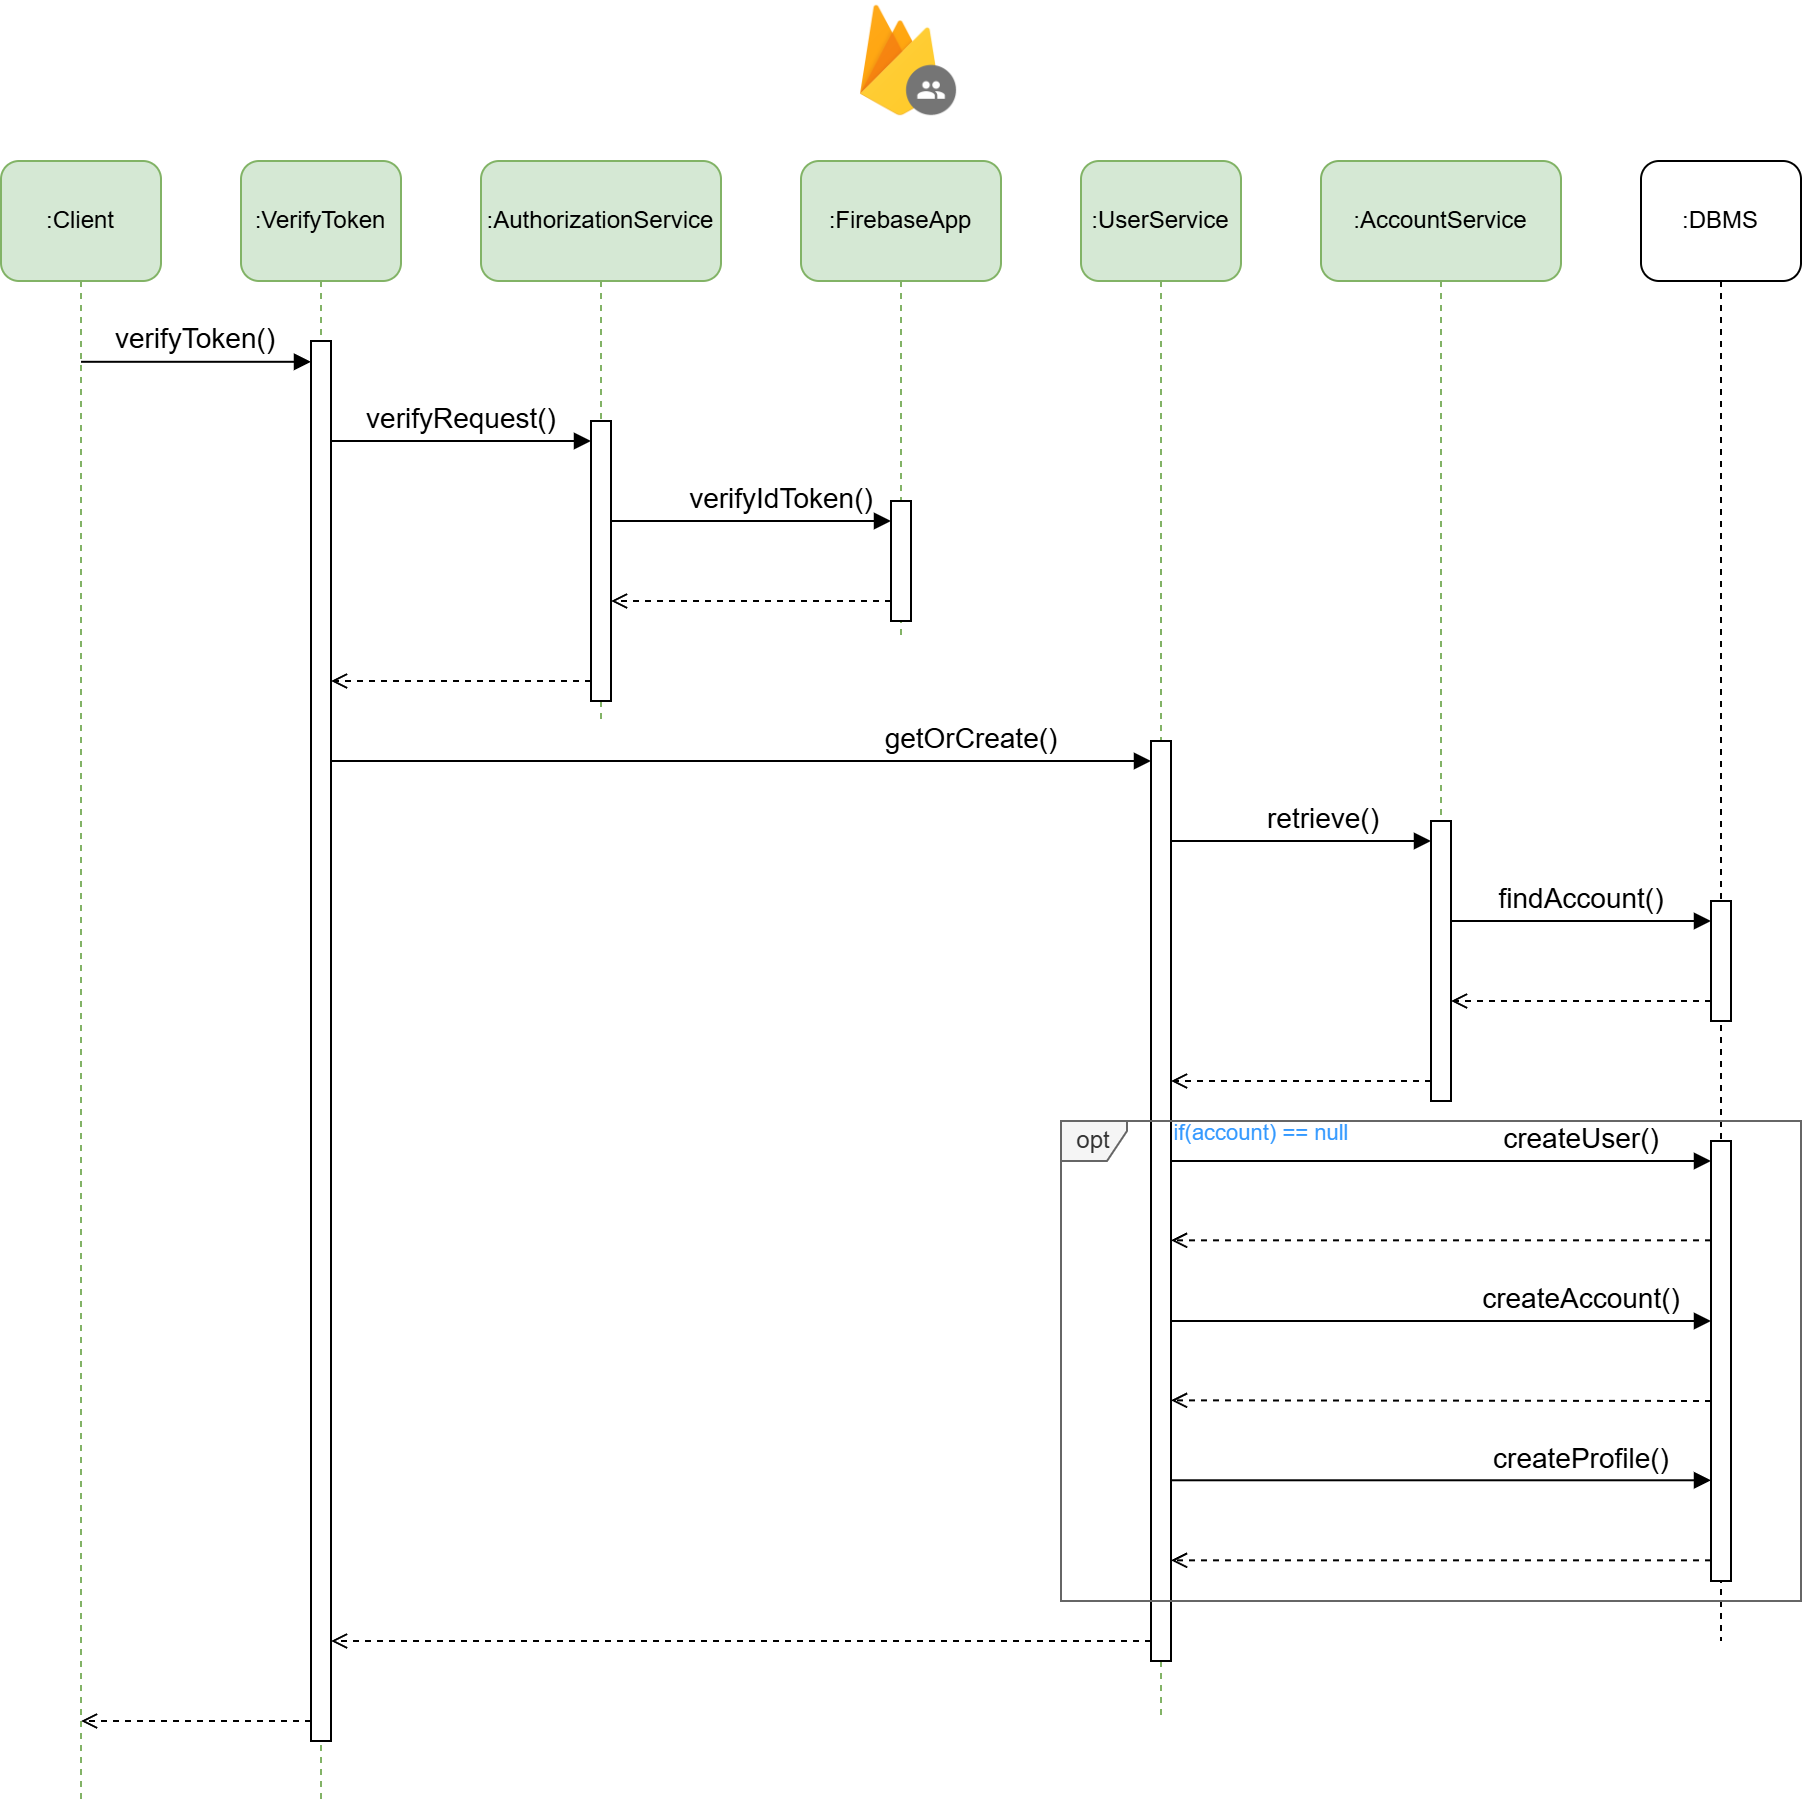
\includegraphics[width=\textwidth]{IIVerifyToken2.png}
    \caption{Diagramma di sequenza per la creazione di un account}
\end{figure}
Per garantire un processo di autenticazione sicuro ed efficiente, a ogni richiesta che richiede identificazione, 
il dispositivo utente aggiunge anche il token di autenticazione, salvato durante il primo accesso e la verifica iniziale. 
Il server verifica quindi la validità del token prima di procedere con l'esecuzione della richiesta.

\clearpage
\subsection{La sicurezza}

Il collegamento tra i vari componenti all’interno dell’ambiente Azure richiede l’utilizzo di chiavi e stringhe di connessione. 
Il salvataggio di tutte le chiavi sensibili è stato affidato al servizio Azure Key Vault,
 un server che permette la centralizzazione dei dati, cifrando il contenuto e garantendo un controllo maggiore sul loro utilizzo. 
Quando necessario i servizi, in particolare le Azure Function, contatteranno il Key Vault per l’ottenimento delle chiavi necessarie, 
riducendo il rischio di un’intercettazione data magari da un errore durante lo sviluppo.\\
\\
Le comunicazioni tra i vari componenti devono avvenire in sicurezza, garantendo autenticità e confidenzialità. 
Per questo motivo tutte le comunicazioni tra dispositivi client e i vari servizi utilizzano la tecnologia TLS, che permette di cifrare i messaggi grazie ad uno standard collaudato. 
In particolare, le comunicazioni tra i client e Azure Function, così come con Firebase Authentication e il server per la persistenza delle immagini, 
avvengono tramite protocollo HTTPS, mentre le comunicazioni con il server per gli aggiornamenti in tempo reale usano il protocollo WSS.\\
\\
L’accesso al database è ristretto alle sole risorse Azure, garantendo l’isolamento dall’esterno, che comprometterebbe altrimenti l’affidabilità dei dati.\\
\\
Infine, l’identificativo di ogni elemento del dominio è nascosto all’utente tramite la creazione di codici hash univoci 
che permettono comunque l’identificazione dell’oggetto senza rivelare ulteriori informazioni. 
In particolare, il caricamento delle immagini avviene grazie ad un link univoco dato dalla combinazione degli identificativi dell’evento e dell’immagine. 
Utilizzando i codici di hash diventa molto complicato il ritrovamento delle immagini senza essere a conoscenza dei codici, 
che non avendo natura incrementale ma distribuita rende indovinare un link valido.

TODO Dos e limite alle dimensioni delle richieste

\clearpage
\subsection{Monitoraggio}

Il monitoraggio del sistema è attuato in due modalità: tramite salvataggio dei log e controllo delle prestazioni del sistema.\\
\\

Relativamente a Firebase Authentication vengono forniti con il servizio sia le interfacce
per il controllo delle prestazioni che la gestione dei log. Non è quindi richiesta alcuna ulteriore azione.\\
\\
Per monitorare le Azure Functions sarà invece necessario collegare Azure Application Insights, servizio che provvede a controllare il funzionamento e la risposta del servizio. 
Una volta unito il servizio, infatti, Azure Application Insight permette la presentazione e l'analisi di numerose metriche, quali il tempo di risposta e il consumo di risorse. 
Consente inoltre di testare la risposta dell’applicativo simulando diversi scenari e riassumendo il loro comportamento.\\
\\
La creazione dei log è invece delegata al programmatore, in quanto è necessario integrarli nel codice. 
Nel momento della creazione, ogni funzione riceve, tramite dependency injection, un servizio Logger che permette la creazione e il salvataggio dei log. 
Tali log saranno poi consultabili e analizzabili tramite l’interfaccia fornita da Azure Application Insight.\\
\\
\clearpage
%\section{ La persistenza}

Nel contesto di un sistema che prevede la gestione di eventi e impegni, è essenziale garantire che l’utente possa accedere in qualsiasi momento alla propria agenda, 
visualizzando gli appuntamenti più urgenti e pianificando efficacemente il proprio tempo. 
Deve perciò essere possibile trovare e mostrare nel minor tempo possibile i dati relativi all’agenda. 
Per soddisfare questo requisito, il recupero e la visualizzazione dei dati devono avvenire con la massima rapidità possibile, 
riducendo i tempi di latenza e ottimizzando il flusso di interazione con l’interfaccia utente. \\
\\
L’adozione di un meccanismo di salvataggio locale sui dispositivi offre il vantaggio di migliorare le prestazioni, 
consentendo un accesso immediato alle informazioni senza dover effettuare continue richieste al server remoto. 
Tuttavia, questa soluzione presenta dei limiti, in quanto non garantisce una persistenza a lungo termine dei dati né assicura la loro disponibilità su più dispositivi. 
Per superare tale criticità, è necessario definire una strategia di gestione della memoria che preveda una fonte di dati centrale e autorevole, 
alla quale tutti i dispositivi possano fare riferimento per recuperare e aggiornare le informazioni in modo coerente e affidabile.\\
\\
Un sistema di persistenza efficace deve quindi prevedere un meccanismo di sincronizzazione tra i dati salvati localmente e la loro controparte ufficiale memorizzata nel database centrale. 
Questo processo deve essere progettato in modo da garantire integrità, coerenza e scalabilità nelle interazioni, 
per essere resistente anche in presenza di un volume significativo di richieste concorrenti. 
La struttura del sistema di memorizzazione deve inoltre essere progettata tenendo conto del dominio applicativo e delle esigenze specifiche di utilizzo, 
al fine di assicurare un bilanciamento ottimale tra efficienza e robustezza operativa.\\
\\
Oltre alla gestione della persistenza dei dati per il singolo utente, è necessario affrontare il problema della condivisione e della modifica collaborativa delle informazioni. 
Poiché l’applicazione consente a più utenti di interagire sugli stessi eventi, le modifiche effettuate da un partecipante devono essere propagate in tempo reale agli altri dispositivi coinvolti. 
Questo introduce la necessità di implementare un sistema di aggiornamento distribuito, in grado di mantenere sincronizzati non solo i dispositivi di un singolo utente, 
ma anche quelli di tutti gli utenti interessati dalle modifiche.\\
\\
La gestione dell’accesso ai dati richiede quindi l’implementazione di un’architettura che preveda un punto di riferimento centrale chiaro e affidabile, 
capace di fungere da fonte primaria delle informazioni. 
Al tempo stesso, l’utilizzo di copie locali dei dati sui dispositivi client consente di ridurre l’impatto delle latenze di rete, 
migliorando la reattività dell’interfaccia e offrendo un’esperienza utente più fluida.\\
\\
L’adozione di una memoria centrale unica garantisce l’integrità e l’affidabilità dei dati ufficiali, 
fornendo un punto di accesso sicuro per la consultazione e la modifica delle informazioni. 
Tuttavia, questa scelta introduce la necessità di gestire due livelli distinti di responsabilità: 
da un lato, il client deve occuparsi di mantenere aggiornati i dati memorizzati localmente, 
mentre il server deve garantire la corretta distribuzione delle modifiche agli altri dispositivi interessati. 
La sincronizzazione e la gestione delle versioni dei dati diventano quindi elementi chiave per assicurare la coerenza del sistema e prevenire eventuali conflitti tra modifiche concorrenti.

\clearpage
\subsection{Memoria principale}

	

Nell’implementazione di applicazioni scalabili, la gestione del salvataggio dei dati può essere strutturata secondo un modello centralizzato o distribuito, 
a seconda delle esigenze di affidabilità, scalabilità e prestazioni del sistema. 
L’adozione di un’architettura di memoria distribuita offre molteplici vantaggi, tra cui una maggiore resilienza ai guasti di una singola fonte, 
la riduzione del carico di memoria su un'unica risorsa di archiviazione e una migliore scalabilità complessiva del sistema. 
Tuttavia, questa soluzione introduce una maggiore complessità infrastrutturale, poiché richiede meccanismi avanzati per garantire la persistenza, 
l’affidabilità e la consistenza delle informazioni.\\
\\
Salvo specifici requisiti che rendano indispensabile la distribuzione totale o parziale della memoria, 
una strategia basata su un database centralizzato può risultare più efficiente dal punto di vista prestazionale e semplificare la gestione complessiva del sistema. 
L’adozione di un’architettura centralizzata consente infatti di ottimizzare i tempi di accesso ai dati e ridurre la latenza delle operazioni, 
a fronte di una minore complessità nella sincronizzazione e nel mantenimento della consistenza delle informazioni.\\
\\
\subsubsection{ I database e la scalabilità}

I database si suddividono in due macro categorie principali: relazionali e non relazionali. 
I database relazionali si caratterizzano per strutture dati rigide e schematizzate, che consentono di stabilire connessioni tra le diverse risorse in tempi estremamente rapidi. 
Viceversa, i database non relazionali offrono una maggiore flessibilità strutturale, permettendo l’archiviazione di dati eterogenei con un accoppiamento più debole tra le entità. 
Questa caratteristica li rende particolarmente adatti a scenari in cui è richiesta un'elevata scalabilità orizzontale e in cui il volume di richieste è significativo.\\
\\

La scelta della tipologia di database più appropriata dipende strettamente dalle esigenze specifiche del progetto. 
I database relazionali sono gli unici in grado di garantire le proprietà di Atomicità, Consistenza, Isolamento e Durabilità (ACID), 
grazie all’implementazione di un rigoroso sistema di transazioni. 
Questo meccanismo, se da un lato assicura un’elevata affidabilità dei dati, dall’altro introduce un temporaneo blocco delle risorse durante le operazioni di scrittura, 
potenzialmente influenzando le prestazioni complessive del sistema.\\
\\
Dal punto di vista della scalabilità, invece, i principali fattori da considerare includono il rapporto tra operazioni di lettura e scrittura, 
la natura dei dati gestiti e la relazione tra le entità. 
Le operazioni di lettura possono essere ottimizzate tramite la creazione di copie dei dati e la parallelizzazione dei processi, 
permettendo di soddisfare un elevato numero di richieste simultanee.\\
\\

Al contrario, le operazioni di scrittura possono introdurre ritardi significativi, in quanto implicano la temporanea indisponibilità della risorsa fino al completamento dell’aggiornamento. 
In alcuni casi, in base alla tipologia del database, ciò può invalidare le copie presenti nel sistema fino alla propagazione dell’aggiornamento, 
compromettendo temporaneamente la consistenza delle informazioni. 
Grazie alla loro struttura flessibile e a requisiti meno stringenti in termini di garanzia ACID, 
i database non relazionali risultano generalmente più efficienti in contesti caratterizzati da operazioni di scrittura frequenti.\\
\\

Quando il sistema richiede una gestione dinamica delle informazioni, con dati opzionali o variabili, i database non relazionali offrono un livello di adattabilità superiore. 
Il salvataggio delle informazioni in forma di documenti consente infatti di modificare la struttura dei dati senza la necessità di riconfigurare lo schema del database, 
garantendo una maggiore elasticità. Tuttavia, questa necessità si manifesta prevalentemente in casi specifici, che rappresentano solo una parte del dominio applicativo complessivo. \\
\\

\subsubsection{La gestione delle relazioni tra le entità}
Un aspetto critico nella scelta del database riguarda la gestione delle relazioni tra le entità. 
È fondamentale analizzare la distribuzione delle richieste per ciascun elemento e il carico computazionale associato a ogni operazione. 
Tra le operazioni più costose in termini di prestazioni, che più ostacola e rallenta il recupero dei dati, vi è l’operazione di unione necessaria. 
Durante le operazioni di unione vengono incrociati i dati di vari elementi per restituire un oggetto coerente che presenti tutte le proprietà necessarie, 
originariamente distribuite in molteplici tabelle. 
L’esecuzione di unione su database relazionali, pur essendo ottimizzata, 
introduce azioni computazionali di grande entità che possono impattare significativamente sui tempi di risposta delle richieste. 
Per questo motivo si cerca di ridurre il più possibile le richieste che comportano l’incrocio di dati da tabelle diverse. \\
\\
Le relazioni tra elementi possono essere classificate in tre categorie principali: 
di tipo uno a uno, uno a molti, e molti a molti. \\
Nelle relazioni uno a uno il recupero dei dati è diretto e richiede uno sforzo computazionale limitato. 
Nei casi uno a molti e molti a molti il reperimento delle informazioni richiede un’attenta valutazione delle modalità di accesso per ottimizzare le prestazioni: 
in questo caso, una delle strategie possibili per migliorare l’efficienza delle richieste offerte dai database non relazionali è il salvataggio per copia del dato all’interno dell’oggetto. 
Questa operazione risulta efficiente se le richieste sono sproporzionate verso una delle due parti.\\
\\
Ad esempio, in una relazione uno a molti, nel caso in cui la richiesta di quell’elemento non sia frequente ma sia importante ottenere gli elementi collegati; 
conviene copiare gli oggetti relativi all’interno dell’elemento singolo. 
L’impostazione inversa, in cui si copia il singolo all’interno dei molti elementi, 
comporterebbe l’ispezione di tutti i componenti esistenti alla ricerca di quelli che contengono l’elemento dato. 
Se però, viceversa, sono frequenti le richieste relative agli elementi multipli, e la loro relazione è importante, 
conviene copiare il singolo all'interno di detti elementi, per evitarne il recupero ogni volta.\\
\\
I database relazionali non permettono la copia di elementi all’interno di altri, ma sono ottimizzati per unire tra loro tabelle, 
richiedendo comunque tempistiche e capacità elaborative non indifferenti. \\
\\
Tuttavia, non vi è alcun vincolo che impedisca l’affiancamento di database di tipologia diversa per rispondere a esigenze specifiche e sfruttare i punti di forza di entrambe le tecnologie.

\subsubsection{ Analisi del dominio}

La scelta del database deriva da un’attenta analisi delle principali interazioni tra gli elementi del dominio. 
Il dominio descrive i componenti dell’applicazione e le loro relazioni. 
In particolare, vengono espresse le dipendenze, i rapporti reciproci e le cardinalità delle relazioni. 
A titolo esemplificativo, dal diagramma del dominio si deduce che ad un oggetto Event possono corrispondere più oggetti Photo, 
ma soprattutto che l’oggetto Photo è strettamente legato all’oggetto Event.\\
\\
\begin{figure}[h!]
    \centering
    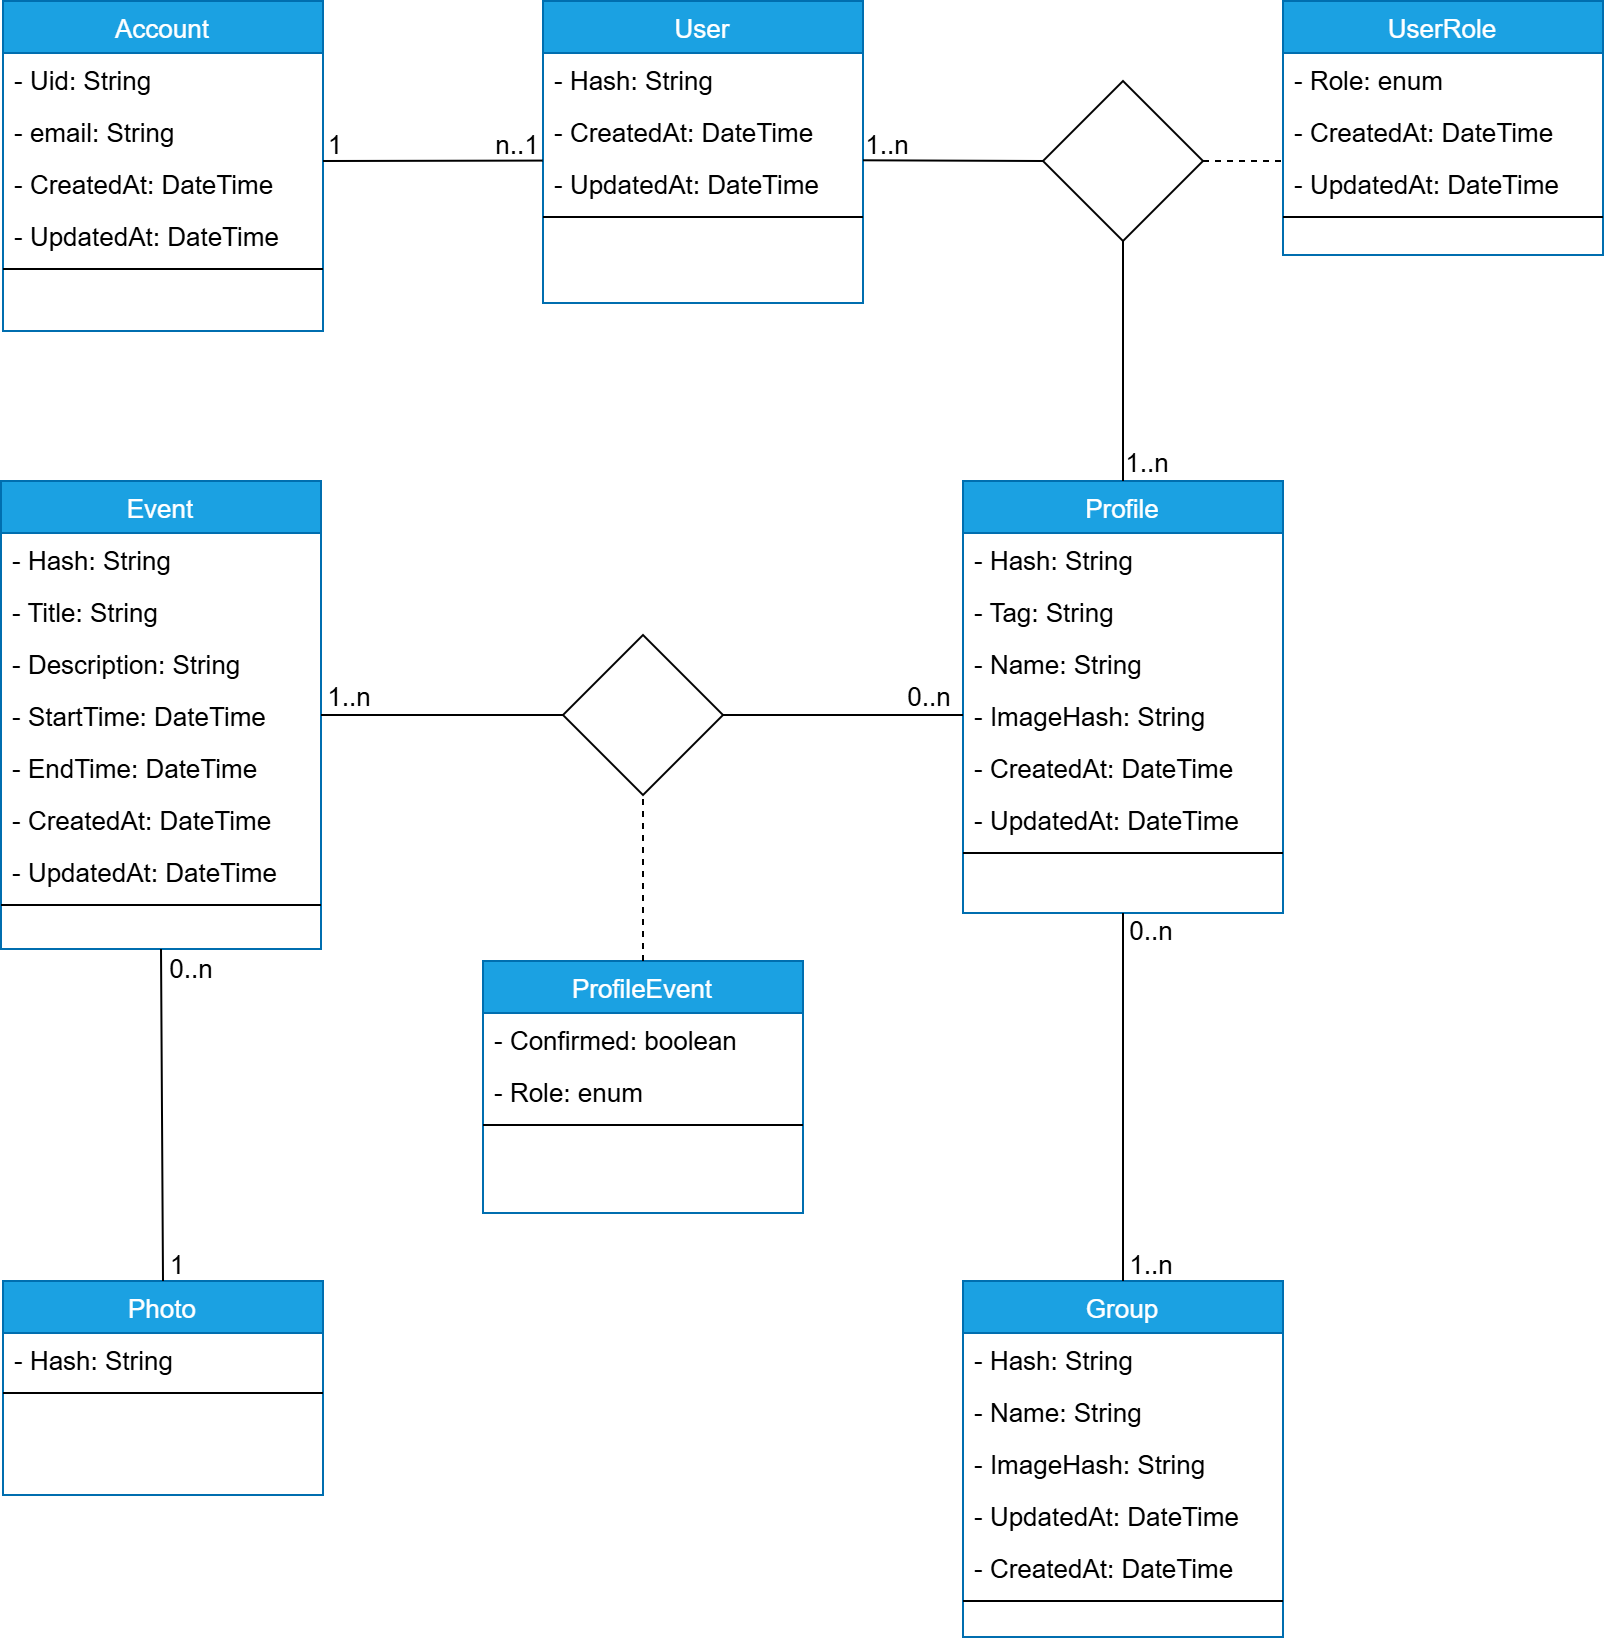
\includegraphics[width=\textwidth]{ProgettoDominioServer.png}
    \caption{ Diagramma del dominio}
\end{figure}
Le richieste riguardo alle informazioni tra Account, User e Profile, con i relativi UserRole, vengono eseguite all’avvio del programma, per poi essere mantenute in memoria locale. 
Le modifiche a questi elementi sono sporadiche.
Allo stesso modo gli oggetti Group vengono recuperati solo all’avvio dell’applicazione, e, salvo rari aggiornamenti, non occupano ulteriormente lo spazio delle richieste.\\
\\
La maggioranza delle richieste verterà sull’ottenimento dei dati relativi agli Event e ai Profile. 
Infatti ad ogni avvio dell’applicazione sarà richiesto di recuperare gli eventi di ogni profilo, mentre, ogni volta che si apre il dettaglio di un evento, 
sarà necessario recuperare i rispettivi dati, includendo i profili associati. 
Si prevede che la cardinalità dei profili associati ad un evento risieda nell’ordine delle decine, 
mentre agli eventi che si associano ai profili l’ordine di grandezza previsto risiede nelle migliaia. \\
\\

La relazione che accomuna Event e Profile è di tipologia molti a molti, identificata con l’oggetto ProfileEvent. 
L’elemento ProfileEvent, oltre a descrivere la relazione, contiene la proprietà Confirmed, che indica la conferma di partecipazione di un profilo ad un evento. 
Vista la natura del progetto, la proprietà Confirmed, assieme ai dati degli Event, sarà tra i campi che subiranno modifiche con maggiore frequenza.\\
\\
Riassumendo, le operazioni principali che vertono sulle prestazioni del database sono il recupero degli eventi relativi ai profili, il recupero dei profili collegati agli eventi, 
l’aggiornamento dei campi degli oggetti Event e la modifica del campo Confirmed relativa ai ProfileEvent.\\
\\

Nonostante sia più probabile che venga richiesto il dettaglio di un evento, e quindi sia più frequente il dover recuperare i Profile relativi all’Event, 
la proporzione delle richieste prevista non giustifica lo sbilanciamento della relazione sugli Event.
Infatti, se si salvassero tutti i ProfileEvent sull’oggetto Event, le richieste degli eventi appartenenti ai profili, sebbene meno frequenti, 
richiederebbero l’ispezione di tutti gli Event alla ricerca del Profile indicato. 
Infine, se si duplicasse l’oggetto ProfileEvent, oltre che nella sua tabella originaria, anche sugli Event la sua creazione, 
la sua eliminazione e la modifica del campo Confirmed richiederebbero il doppio delle scritture.\\
\\
Vista quindi la necessità di letture frequenti da entrambe le parti di una relazione molti a molti e la necessità di scrittura dell’oggetto che la identifica, 
si individua in un database relazionale la soluzione più efficace per il dominio del progetto. 
Infatti, i database relazionali sono ottimizzati sulle operazioni di unione tra tabelle, garantendo velocità di recupero in lettura da entrambe le parti. 
Permettendo la separazione delle tabelle e gestendo gli oggetti ProfileEvent come entità indipendenti, 
la modifica del campo Confirmed comporta il blocco del solo elemento ProfileEvent. 
Le caratteristiche ACID forniscono inoltre uno stato centrale per tutta l’applicazione, che, 
per quanto non strettamente necessario, garantisce l’uniformità delle informazioni per tutti gli utenti.\\
\\

\clearpage
\subsubsection{La salvandocelta del database}

Azure offre un’ampia scelta di database relazionali che possono essere integrati con il resto dell’ecosistema. 
Oltre alla tecnologia proposta, nella scelta del database più adatto bisogna considerare soprattutto l’integrazione con servizi accessori, 
le particolarità del server su cui viene eseguito, e i costi che si andrà ad affrontare.\\
\\
\begin{figure}[h!]
    \centering
    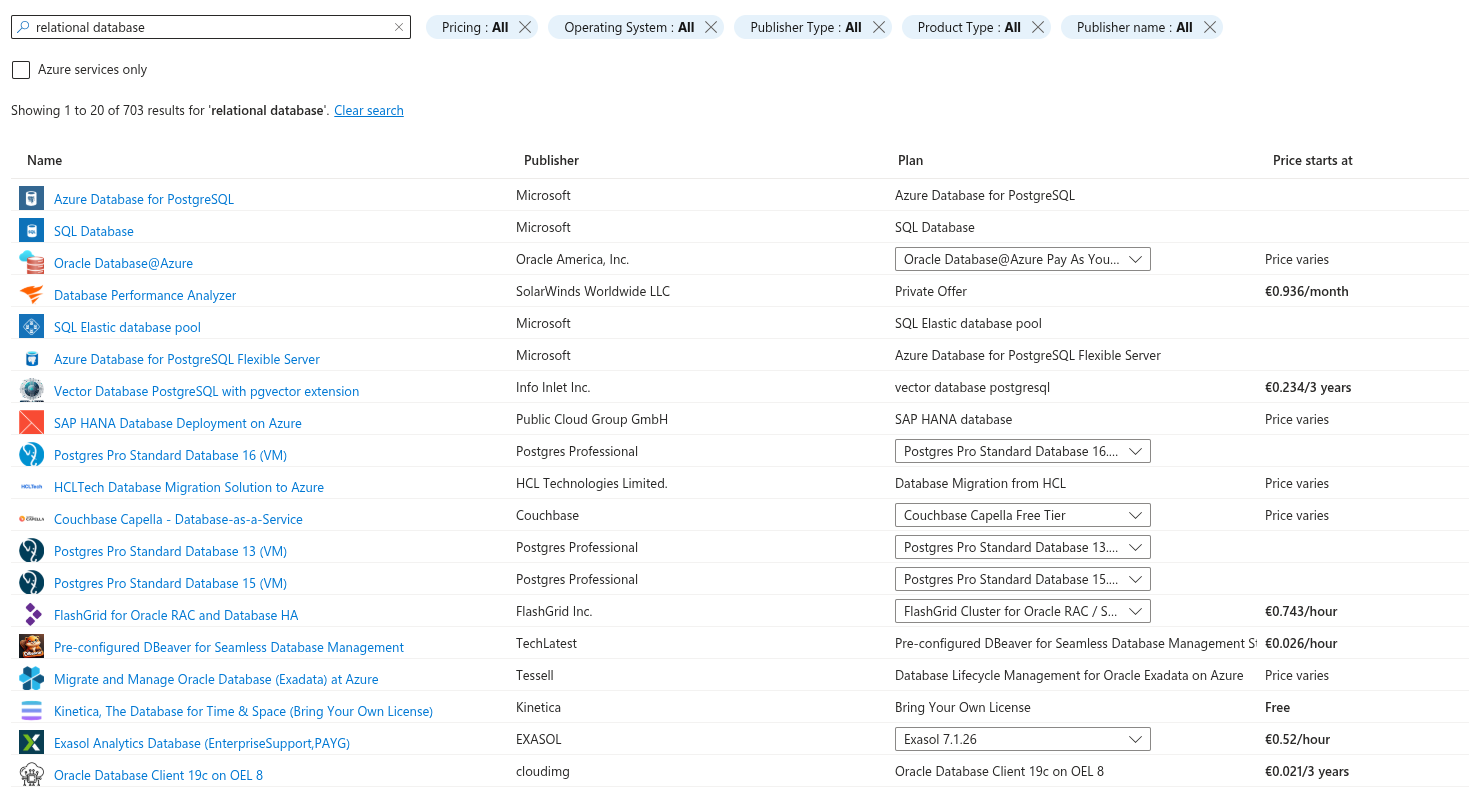
\includegraphics[width=\textwidth]{Possibilitadelcloud.png}
    \caption{Proposte di Azure per i database relazionali}
\end{figure}	


A meno di necessità particolari che richiedono l’utilizzo di una tecnologia implementata da uno specifico database, 
la grande sovrapposizione di funzionalità delle diverse offerte di database relazionali presenti sul mercato garantisce 
il  soddisfacimento delle necessità rilevate dall’analisi del dominio indipendentemente dalla tecnologia proposta dal servizio.\\
\\
La grande differenza tra i vari servizi sta nelle proprietà del server incaricato di fornire il potere computazionale necessario per l’esecuzione. 
L’architettura del server e la sua integrazione con la tecnologia del database, infatti, determinano l’effettiva capacità di scalabilità del servizio.\\
\\
Si intende scalabilità verticale la capacità di aumentare le risorse della stessa macchina in cui si esegue il codice. 
La scalabilità verticale viene definita nel momento di creazione del servizio, in cui si determinano le risorse da dedicare alla macchina che esegue il programma. 
Trattandosi di macchine virtualizzate, è sempre possibile in un secondo momento aumentare le prestazioni in caso di necessità.\\
\\

Per scalabilità orizzontale si intende invece la capacità di delegare il carico di lavoro ad altre macchine, eventualmente coordinando le modifiche. 
Questo permette una risposta alle richieste più resistente, riducendo il rischio di colli di bottiglia che potrebbero venirsi a formare nell’utilizzo di un nodo singolo.
La scalabilità orizzontale richiede però l’implementazione di tecnologie apposite integrate con il database che permettano l’esecuzione in nodi fisici differenti. \\
\\
Una volta individuata la tecnologia adatta e il livello di scalabilità desiderati, 
è bene considerare le altre necessità o le opportunità aggiuntive generate dalla presenza di un database nel progetto. \\
\\

L’alta disponibilità(HA) è la proprietà di garantire l’accesso al servizio nonostante i guasti. 
Ad esempio, si può mantenere una macchina identica al server principale in grado di replicare il servizio, spostando il carico in caso di guasto del server principale. 
Si misura in “numero di nove”, ovvero la quantità di nove presenti nella percentuale del tempo per il quale si garantisce la disponibilità del servizio.
I servizi offrono diverse qualità di HA, in base alle funzionalità desiderate.\\
\\

Alcuni servizi possono presentare offerte di backup per riportare il server nello stesso stato di qualche momento precedente. 
Questo permette il ripristino del sistema ad un punto precedente rispetto all’avvenimento di eventuali errori o guasti del sistema.\\
\\

Inoltre, Azure mette a disposizione molteplici servizi accessori che possono essere uniti al servizio. 
Questo permette di estendere le potenzialità del database tramite  l’analisi e il monitoraggio dei dati, 
generando prestazioni aggiuntive o integrando i dati per lo sviluppo di altre tecnologie.\\
\\
Infine è necessario controllare i costi che le scelte progettuali e prestazionali hanno comportato: 
pur generalmente legati al consumo effettivo delle risorse, e quindi in grado di fornire solo una previsione del costo finale, 
ogni decisione presa conduce ad un possibile aumento di prezzo, 
ed è quindi bene controllare che le risorse selezionate siano effettivamente  necessarie a soddisfare i requisiti del progetto.\\
\\
Riducendo al minimo i costi, visto l’utilizzo iniziale dell’applicazione, e nessuna necessità tecnologica specifica, 
la scelta del database per la persistenza del progetto è ricaduta su Azure SQL Database. 
Presentando un database relazionale di tecnologia proprietaria di Microsoft, Azure SQL database esegue su un solo nodo, 
fornendo però la possibilità di  scalare  verticalmente tramite la possibilità di modificare le risorse assegnate in ogni momento, 
garantendo comunque prestazioni soddisfacenti per il servizio.\\
\\
Al server principale è stata affiancata una replica che rimane costantemente aggiornata. 
Situata in una località differente dal server principale, garantisce alta disponibilità continuando a fornire i servizi anche in caso di malfunzionamenti al server principale.
\clearpage
\subsubsection{ Le limitazioni dei database relazionali}

La scelta di un database relazionale può però comportare limitazioni a livello prestazionale. 
Il più grande tallone d'Achille dei database relazionali è il numero limitato di connessioni contemporanee permesso. 
Questo comporta un numero massimo di richieste in contemporanea che il database può gestire, minacciando la scalabilità. \\
\\

Per ovviare ai problemi di scalabilità ci sono diverse soluzioni non esclusive che possono migliorare le prestazioni. 
Sicuramente si deve limitare al minimo il tempo in cui ogni richiesta mantiene la connessione, 
distinguendo nel codice momenti precisi e definiti in cui vengono richieste le modifiche al database. \\
\\  

Inoltre, si può interporre un livello di caching tra la logica applicativa e le richieste al database. 
Il livello di caching si occupa di gestire le richieste al database fornendo e duplicando le risposte che possiede già in memoria, 
eventualmente centralizzando le richieste in caso i dati siano invece da recuperare. 
Per i dati in scrittura, invece, salva temporaneamente le modifiche richieste, aggiornando subito la memoria locale, 
per poi apportare le modifiche al database in momenti di carico ridotto. 
Garantisce così un tempo di risposta e di propagazione degli aggiornamenti ridotto. 
Questo consente di alleviare le richieste al database, estendendo di molto le prestazioni fornite.\\
\\

Nel caso in cui però fossero necessarie ulteriori prestazioni, se il dominio e i requisiti lo permettono, 
si può eventualmente delegare ad un database non relazionale le modifiche ai dati e alle relazioni che non necessitano delle qualità ACID ma richiedono un’alta frequenza di scrittura.\\
\\ 
Infine, se fosse necessario mantenere un database relazionale, 
per aumentare le prestazioni conviene cambiare architettura e adottarne una che supporti la scalabilità orizzontale, per suddividere il carico su più nodi.
\clearpage


\subsubsection{L' integrazione con C\#}

La scelta di un database relazionale per la persistenza ha comportato sviluppi progettuali precisi. 
In primis si rende necessario tradurre il dominio in componenti relazionali che possano essere espressi e salvati nelle tabelle del database.

\begin{figure}[h!]
    \centering
    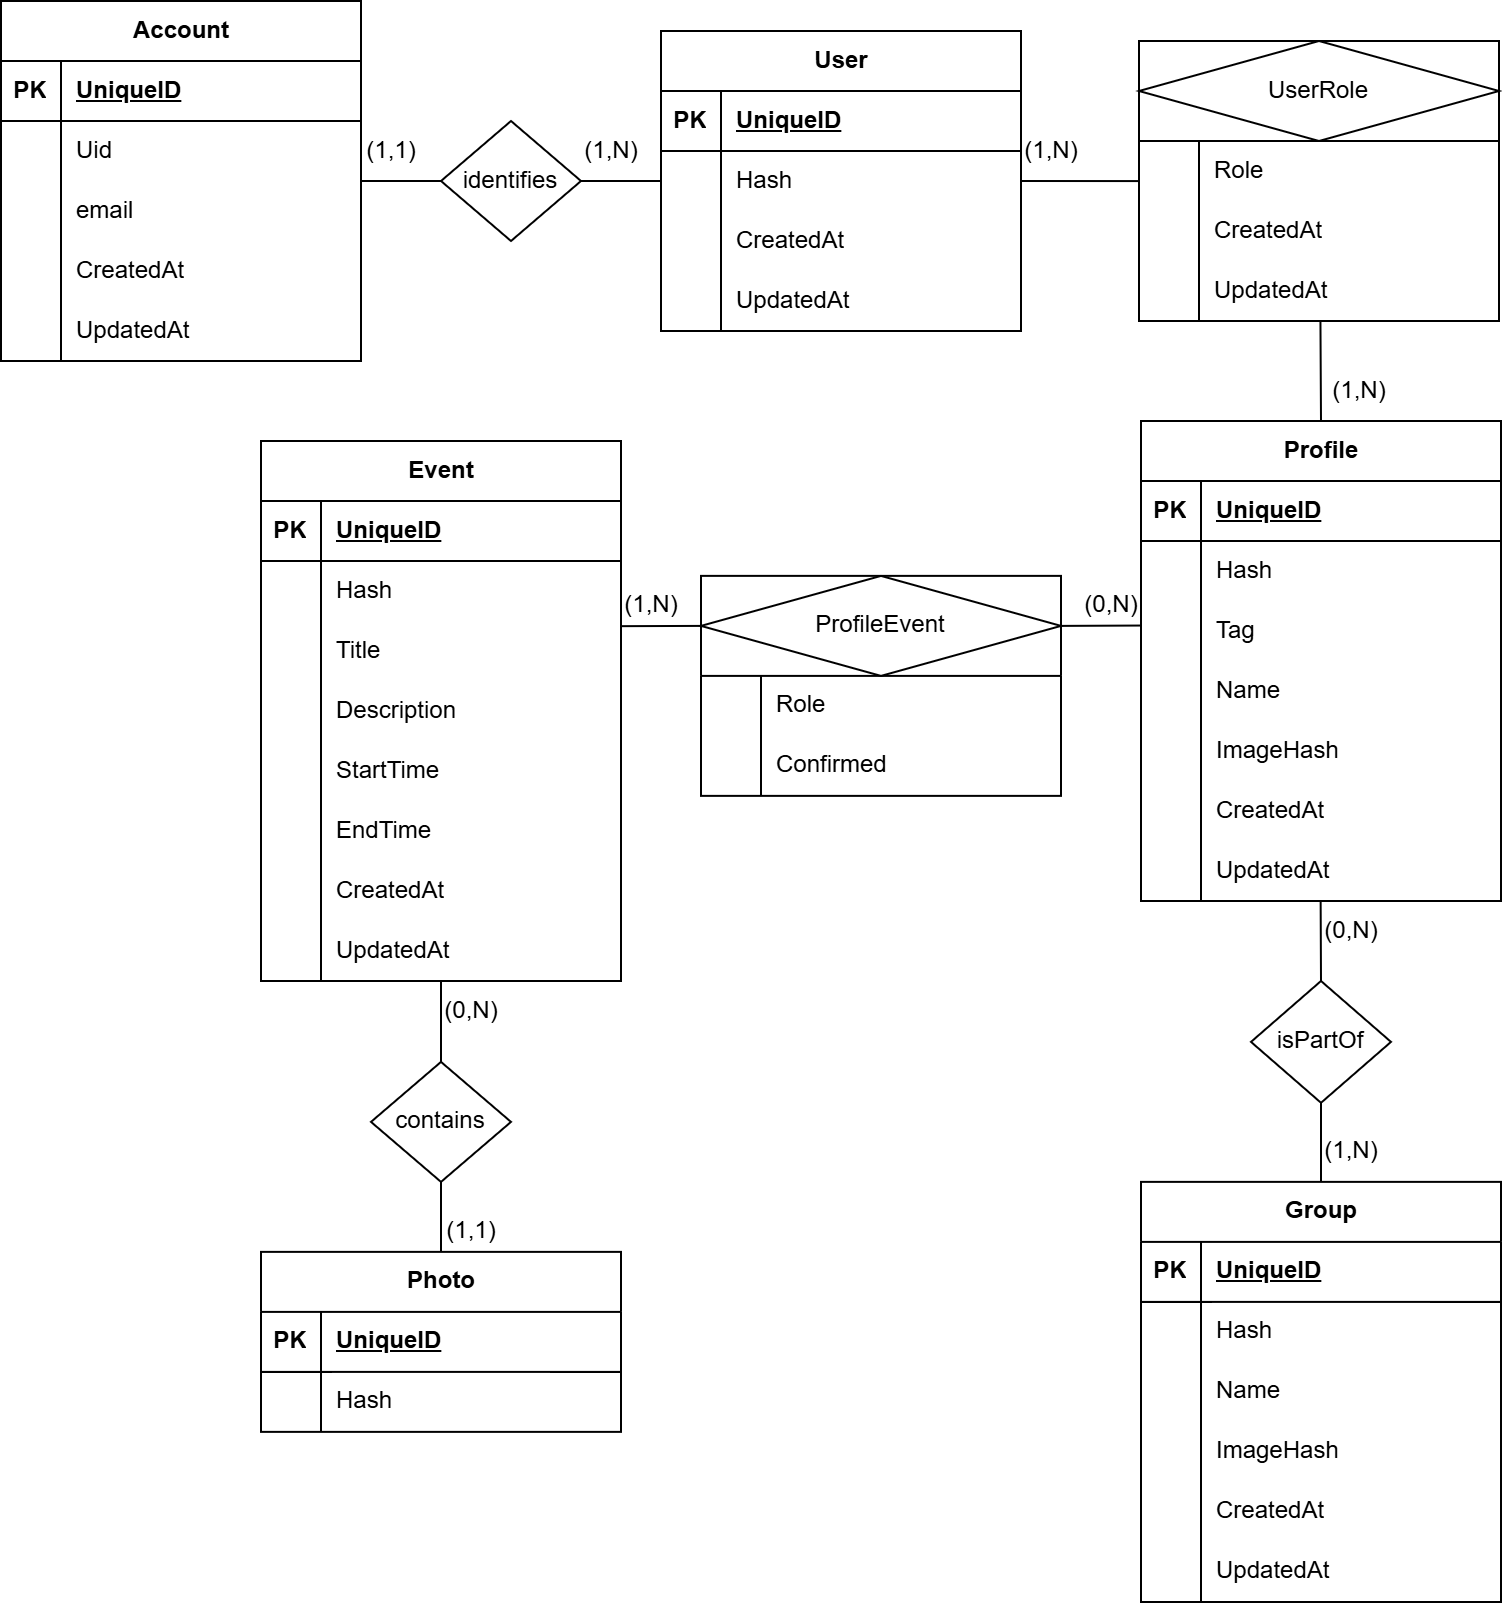
\includegraphics[width=\textwidth]{ProgettoDiagrammaER.png}
    \caption{Diagramma Entità - Relzione del dominio}
\end{figure}	

Si creano quindi sul server le classi logiche del programma, a partire dal dominio. 
Ogni classe corrisponde ad un oggetto del dominio, presentando i valori e le relazioni dei componenti come attributi dell’oggetto.\\
\\
Entity Framework Core di .Net(EFCore) è una libreria di C\# che permette di unire le classi logiche del programma alle tabelle del database. 
Fornisce un’astrazione logica del collegamento con il database e le richieste relative, fornendo una rappresentazione di alto livello delle connessioni sottostanti. \\
\\
Una volta collegato il server con il database tramite le stringhe di connessione salvate sull’Azure Key Vault, 
sono state definite le proprietà tra le varie entità, per poi inizializzare in automatico la struttura del database. 
Le modifiche alla struttura del database vengono infatti generate automaticamente da EFCore in seguito alla creazione o alla modifica degli attributi degli oggetti. 
Questo permette di star dietro agli aggiornamenti, generando e salvando le modifiche da applicare ad ogni modifica delle proprietà del dominio.\\
\\
\begin{figure}[h!]
    \begin{center}
        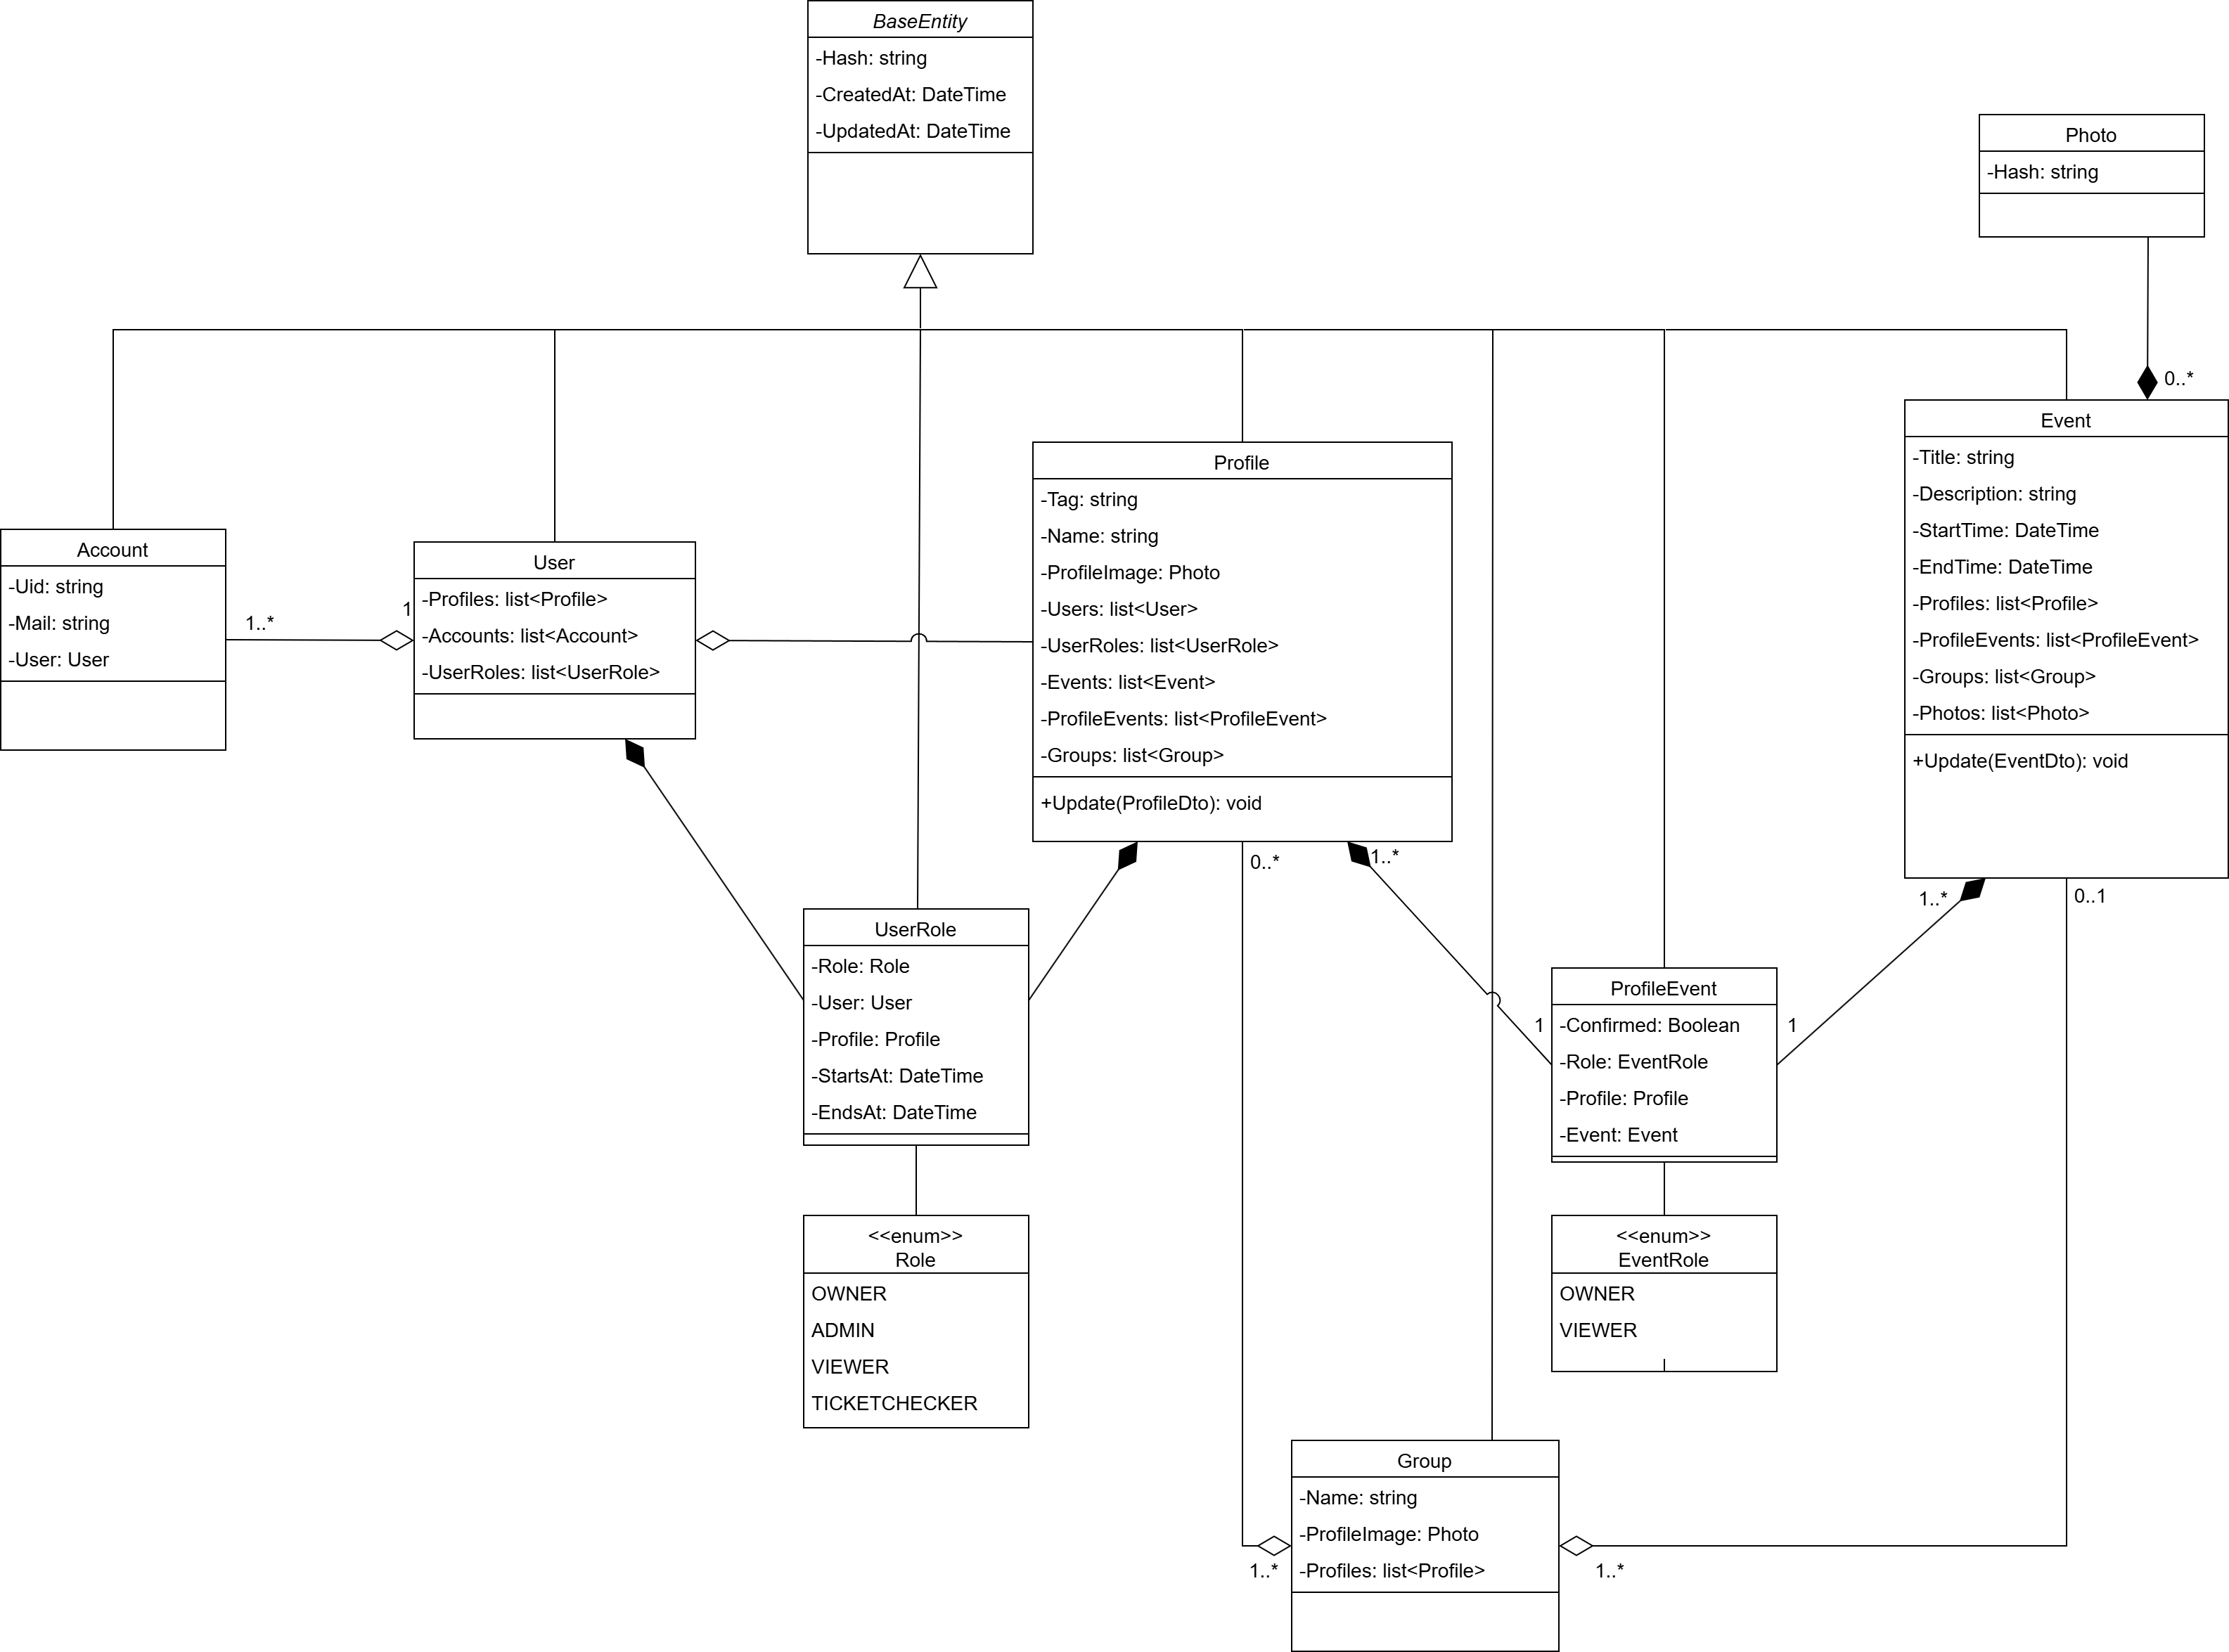
\includegraphics[width=\textwidth]{ModelClassDiagram.png}
        \caption{Modello delle classi del client}
    \end{center}
\end{figure}

Per la riduzione del carico computazionale richiesto da elementi con tante relazioni si utilizza la tecnica del lazy loading. 
La tecnica del Lazy Loading consiste nel richiedere i dati delle relazioni di un elemento solo quando strettamente necessario. 
La sua realizzazione tramite EFCore è attuata grazie alla proprietà virtual, 
che permette di gestire un oggetto con un riferimento al database richiedendo i dati delle sue relazioni solo quando viene espressamente richiesto.
\clearpage
\subsection{ Cache Locale}

Richiedere e ottenere dati dal server comporta ritardi che impattano sulle prestazioni. 
Se la tecnologia del dispositivo lo permette, è utile salvare copie delle informazioni usate più frequentemente nella memoria locale del dispositivo. 
Nel momento di una interazione che richiede la ricerca dei dati, si possono fornire le informazioni disponibili in copia, 
per poi eventualmente aggiornarle se si rivelassero imprecise. Questo permette un tempo di risposta apparente minore e una migliore esperienza utente.\\
\\
\subsubsection{ Creazione della memoria locale}
Non tutti i dispositivi permettono una gestione della memoria a lungo termine. 
In particolare, i browser web non presentano questa funzionalità, ma i dispositivi mobili e i programmi sì. \\
\\
Per motivi di prestazioni, il framework Flutter nativamente mantiene lo stato di un componente solo il tempo strettamente necessario per la sua esecuzione. 
Il tempo di vita dello stato coincide normalmente con quello del componente a cui è associato. 
La normale persistenza degli elementi e dei dati ha durata limitata. 
Si rende necessaria la creazione e la gestione di una cache locale che permetta di mantenere i dati ricevuti dal server anche in seguito al termine di servizio dei componenti.\\
\\
\begin{figure}[h!]
    \centering
    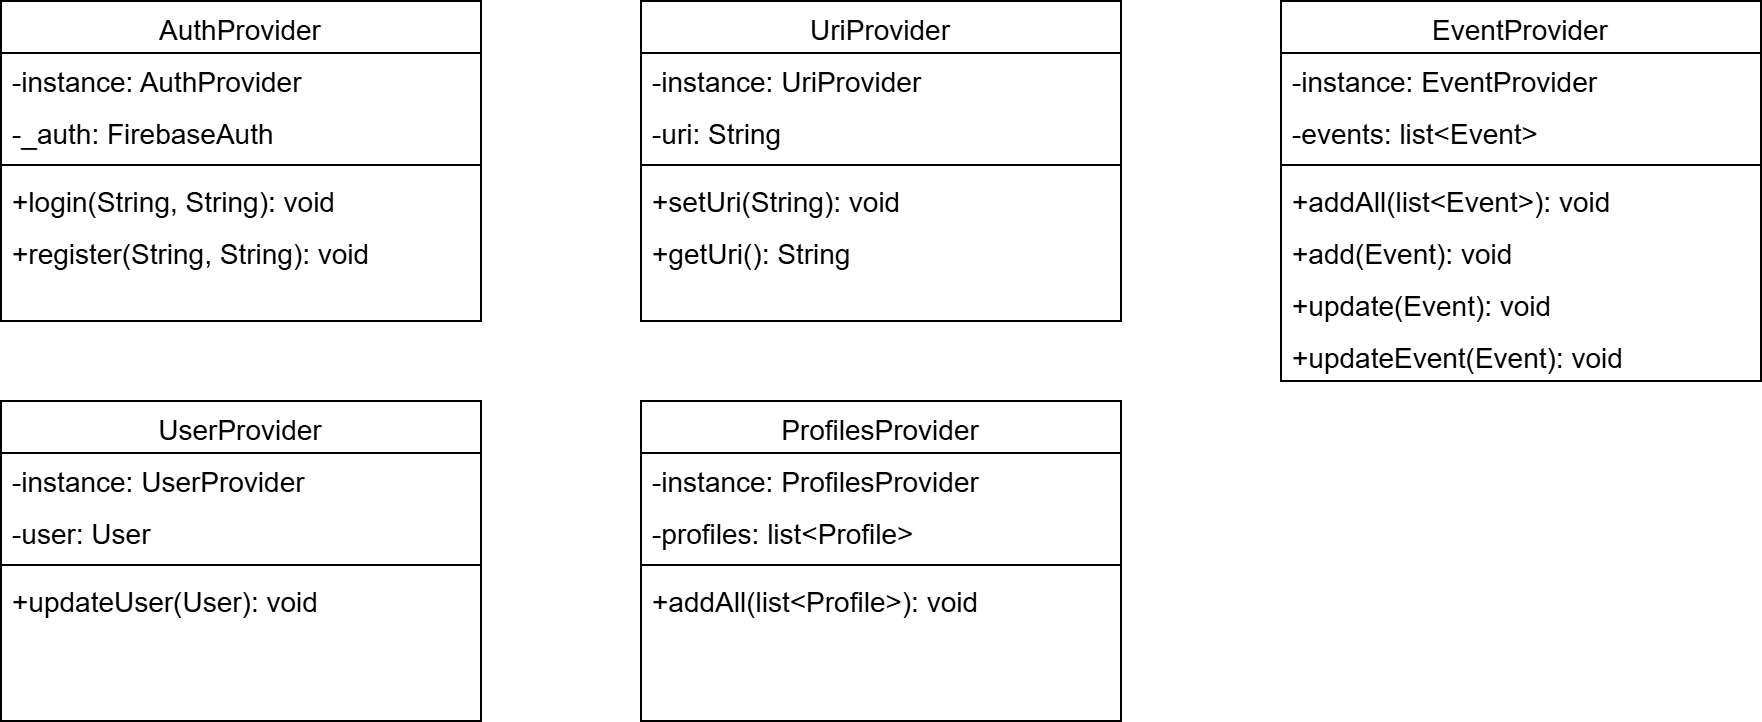
\includegraphics[width=\textwidth]{FrontProviderClassDiagram.png}
    \caption{Classi provider all'interno dell'applicazione}
\end{figure}	
La cache locale viene suddivisa in base alle classi logiche del dominio, ed è accessibile tramite servizi dedicati. 
In particolare, grazie a componenti di tipologia provider è possibile aggiornare in automatico le parti dell’applicazione interessate dalle modifiche. 
Al termine di una richiesta dati al server, il provider viene notificato, salvando il dato in memoria e scatenando un aggiornamento a catena sui componenti interessati.\\
\\
La cache deve essere unica e disponibile in tutto il programma. 
I provider attraverso cui si realizza la cache locale seguiranno il pattern singleton, che garantisce l’unicità dell’elemento all’interno del programma. 
Una volta creati all’avvio del programma, infatti, tutti gli elementi dell’applicazione avranno accesso agli stessi dati, quando necessario.

\begin{figure}[h!]
    \centering
    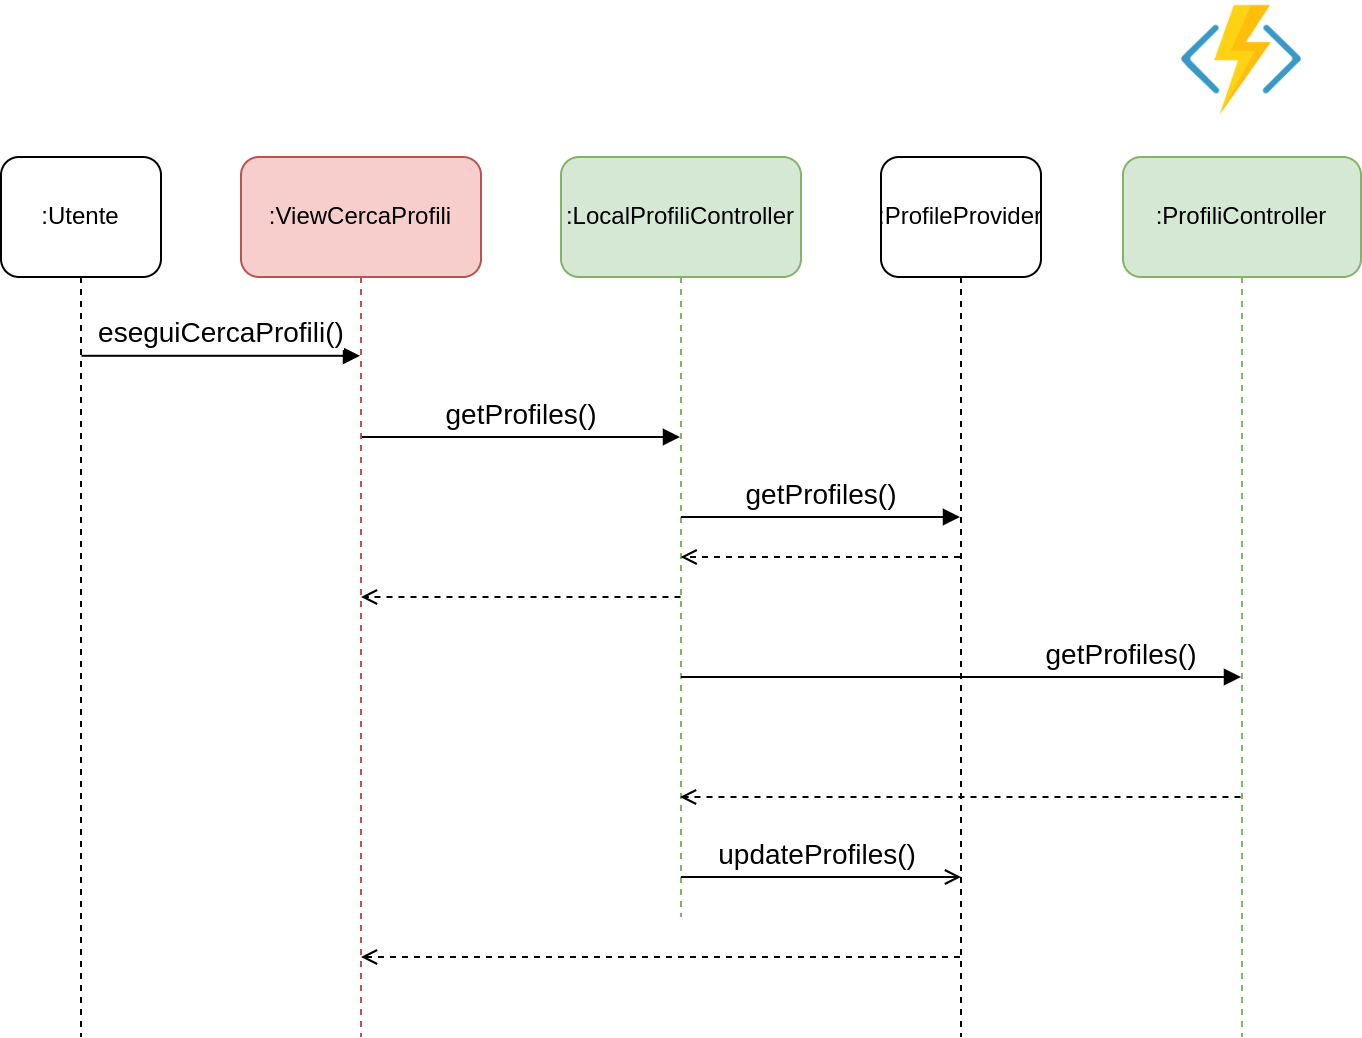
\includegraphics[width=\textwidth]{Providers.png}
    \caption{Esempio di interazione logica tra i componenti del client}
\end{figure}	

eventualmente salvataggio delle modifiche offline per caricarle quando si torna online. \\
\clearpage
\subsubsection{ L'allineamento con la memoria centrale}

il client ha la responsabilità di tenere allineata la propria cache ai valori della memoria centrale. 
Per quanto possa fare temporaneamente affidamento sulle risorse che ha salvato in cache per ridurre i tempi di risposta con l’utente, 
la loro validità dipende dalla certezza che corrispondano ai dati ufficiali. \\
\\

Ogni elemento avrà associato l’ultimo momento in cui è stato aggiornato. 
Allo stesso modo, viene salvato l’ultimo momento in cui è stata attivamente effettuata una richiesta esplicita di aggiornamento.  
Ad ogni avvio dell’applicazione il client invierà una richiesta al server per ricevere tutti gli elementi che hanno subito modifiche successivamente al momento dell’ultimo aggiornamento.\\
\\
La necessità di avere aggiornati tutti gli elementi della cache nel minor tempo possibile dipende anche dalla tipologia dell’elemento. 
Bisogna identificare gli elementi per il quale l’allineamento è critico per il corretto funzionamento dell’applicazione, 
come invece quelli che svolgono ruoli secondari e possono essere aggiornati anche in un secondo momento. 
Ad esempio, la modifica della durata di un evento è necessario venga rilevata il prima possibile, 
mentre la modifica della foto associata ad un profilo ha vincoli di aggiornamento in memoria locale molto più rilassati.\\
\\
Nel caso di dati critici si implementa un meccanismo che esegue, periodicamente, una richiesta degli elementi modificati nell’arco di tempo dall’ultimo aggiornamento, 
per poi aggiornare il loro valore. Invece, nel caso di elementi secondari, 
si possono richiedere allineamenti direttamente nel momento in cui vengono posti espressamente in attenzione dato l’utilizzo dell’app.

\clearpage
\subsection{Aggiornamenti}

Data la natura condivisa dell’applicazione risulta fondamentale che gli utenti siano aggiornati in tempo reale sulle modifiche applicate agli eventi, 
oltre ad essere una prerogativa di tutte le applicazioni moderne, anche per migliorare la user experience. 
Lo spostamento di un appuntamento, la conferma di una presenza o la modifica del luogo di appuntamento sono elementi critici che è bene che gli utenti vengano informati il prima possibile. \\
\\
Il cloud fornisce strumenti per il supporto e lo sviluppo di queste funzionalità, ma, oltre a dover individuare la tecnologia più adatta, bisogna anche essere in grado di integrarla nel resto del progetto.\\
\\
\subsubsection{ Scelta della tecnologia}


La comunicazione con il server finora implementata si basa sul protocollo Hypertext Transfer Protocol (HTTP). HTTP prevede un fornitore di servizi (il server) mettere a disposizione una porta ad un indirizzo fisso rimanendo in attesa di eventuali utilizzatori (client) che, interfacciandosi attivamente alla porta disponibile,  espongono le loro richieste.
La riduzione delle comunicazioni al minimo indispensabile, oltre a non richiedere al server alcuna conoscenza del client, rende il protocollo pratico e scalabile.

Questa dinamica però impedisce ai client di essere notificati di eventuali modifiche apportate, a meno di richieste periodiche frequenti che comportano un sovraccarico da entrambe le parti. Inoltre, l’inversione dei ruoli non è applicabile in quanto i client cambiano costantemente l’indirizzo a loro associato, così come è impossibile distinguere se il dispositivo abbia terminato la connessione o se sia un guasto di altro tipo. 

Si necessita una comunicazione che mantenga in costante contatto i client con le modifiche del server, permettendo una trasmissione attiva degli aggiornamenti.
A basso livello, il protocollo che permette una comunicazione continua più adatto alle tecnologie comunemente diffuse è quello delle WebSocket. Tramite WebSocket infatti si crea un canale diretto tra le parti che consente una comunicazione istantanea. 

Alla necessità di supportare il protocollo delle WebSocket e di inviare istantaneamente i messaggi, si aggiunge la possibilità di creare molteplici canali specifici per indirizzare correttamente le comunicazioni ai soli interessati.


\begin{figure}[h!]
    \centering
    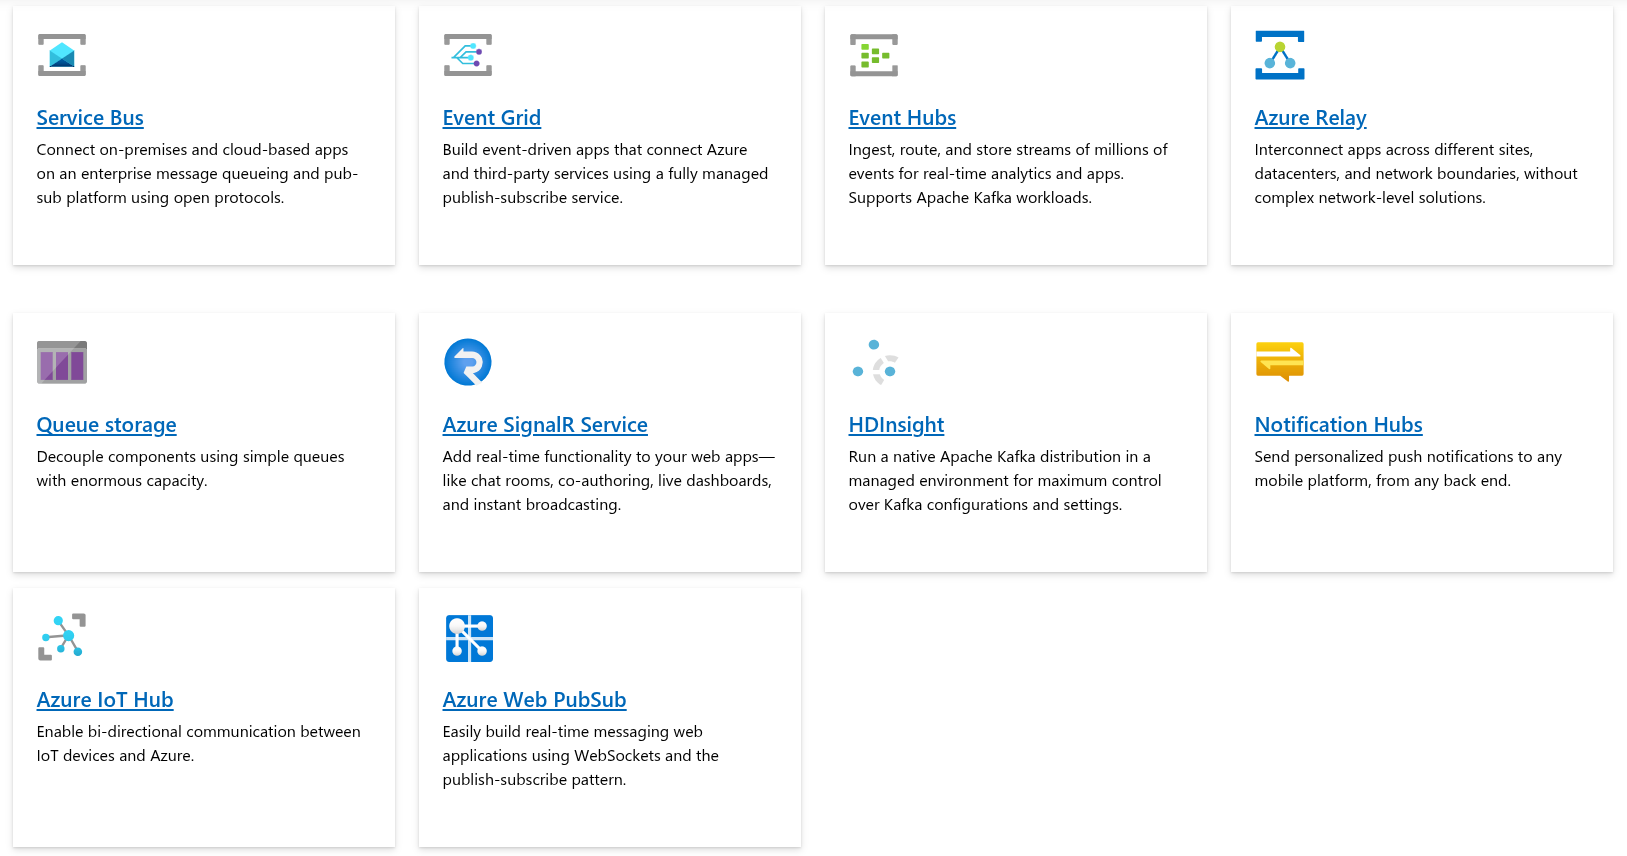
\includegraphics[width=\textwidth]{AzureMessagingServices.png}
    \caption{I servizi di comunicazione istantanea proprietari di Azure}
\end{figure}	


Per individuare la tecnologia più adatta ad aggiornare gli utenti, tra le tante che offrono servizi di collegamento istantaneo tra tecnologie, è fondamentale comprendere  gli scopi per cui sono nate e che problemi quindi risolvono. Infatti, ogni servizio è stato progettato per affrontare specifiche sfide che si differenziano sia per la natura dei servizi a cui si rivolgono che per  modalità di approccio .

La natura degli attori per cui il servizio si specializza determina le prestazioni di scalabilità e le integrazioni supportate. Bisogna quindi considerare la località e la natura delle risorse: in-premise o sul cloud, se appartengono alla stessa piattaforma o se devono comunicare internamente.
Ad esempio, un servizio pensato per collegare tantissimi dispositivi distribuiti con limitato potere computazionale, come nel caso dell’Internet of Things, fornirà  supporto a connessioni esterne e a protocolli standard, e prevederà un’elevata quantità di richieste di limitate dimensioni e frequenza. Viceversa, la necessità di creare una comunicazione tra un numero ristretto di server con prestazioni elevate comporta la creazione di flussi di dati importanti, magari gestiti internamente all’ambiente cloud, astraendo la tecnologia necessaria.

I servizi si differenziano però anche per le caratteristiche delle connessioni gestite.
Proprietà fondamentale è la natura delle comunicazioni. I canali possono essere infatti unidirezionali, permettere la comunicazione da entrambe le parti o implementati come flussi di eventi, in cui le comunicazioni possono essere inviate e ricevute da molteplici attori, senza che il destinatario sia noto al mittente. Inoltre, alcuni servizi offrono la possibilità di individuare categorie di clienti specifiche a cui eventualmente inviare notifiche mirate. Infine, bisogna prendere in considerazione la necessità di persistenza delle comunicazioni, che fornisce, oltre all’aggiornamento in tempo reale, anche la possibilità di recuperare modifiche passate.

Nel progetto si necessita di un servizio che supporti le WebSocket e che permetta di creare una molteplicità di canali unidirezionali differenti. In particolare, deve essere il più indipendente possibile dagli attori con cui comunica per poter garantire il maggior supporto possibile. Dovendo coprire solo le notifiche di aggiornamento, senza responsabilità di rintracciabilità dei dati, la presenza della persistenza non è necessaria.

Gratuito per le prime 20 connessioni, ma eventualmente scalabile per soddisfare ulteriori carichi, il servizio individuato per la gestione delle notifiche in tempo reale è Azure Web Pub Sub (AWPS). Permette infatti la creazione di canali tramite WebSockets e l’integrazione con le Azure Function. Supporta la creazione di canali, sia unidirezionali che bidirezionali, su cui pubblicare eventi, a cui gli utenti possono collegarsi per ricevere gli aggiornamenti. Non prevede l’utilizzo di persistenza ma gestisce completamente la scalabilità e l’affidabilità del sistema.



\subsubsection{Integrazione}

L’integrazione di Azure Web Pub Sub deve avvenire sia con il server che con i devices degli utenti. Seguendo il modello publish subscribe, ogni client si connetterà ad un canale in sola lettura, ricevendo tutti i dati che verranno pubblicati su di esso. Il server avrà il compito di interfacciarsi con il servizio per pubblicare i dati sui canali interessati.

La scelta della definizione del canale deriva da un’ulteriore analisi del dominio. 
Il soggetto interessato alle modifiche sottoposte a notifica è il profilo. 
Se però si creassero i canali in relazione ai profili ogni dispositivo (che riassume l’interazione di un utente) dovrebbe mantenere una connessione per ogni profilo collegato all’utente. La creazione di un canale per ogni device allo stesso modo risulta estremamente inefficiente, in quanto, oltre ad introdurre nuovi requisiti per garantire la tracciabilità dei dispositivi, ne richiederebbe di creazione e gestione in numero elevato. Per queste ragioni i canali verranno creati uno per utente, garantendo inoltre che gli unici utenti a ricevere le notifiche ne posseggano effettivamente l’accesso adeguato.

A seguito di una richiesta che comporta la notifica ai profili interessati, il server avrà il compito di interfacciarsi con AWPS per affidargli le comunicazioni relative. Tuttavia AWPS non supporta la capacità di unire gli elementi in base alle loro relazioni, per cui la responsabilità di trovare gli utenti interessati ricade sul server. 
Ad esempio, la modifica di un evento comporta la notifica a tutti i profili relativi, e quindi una comunicazione a tutti gli utenti che ne posseggono i permessi di notifica per la particolare azione su detti profili. 

L’operazione di ottenimento degli utenti coinvolti data l’azione svolta (nell’esempio, la modifica di un evento) verrà eseguita in un’altra Azure Function dedicata che si occuperà poi, per ogni utente coinvolto, di comunicare  al server AWPS il messaggio da notificare. L’eventuale fallimento della operazione viene inserito tra i log e risulterà durante i monitoraggi, senza coinvolgere la funzione principale.

		
\begin{figure}[h!]
    \centering
    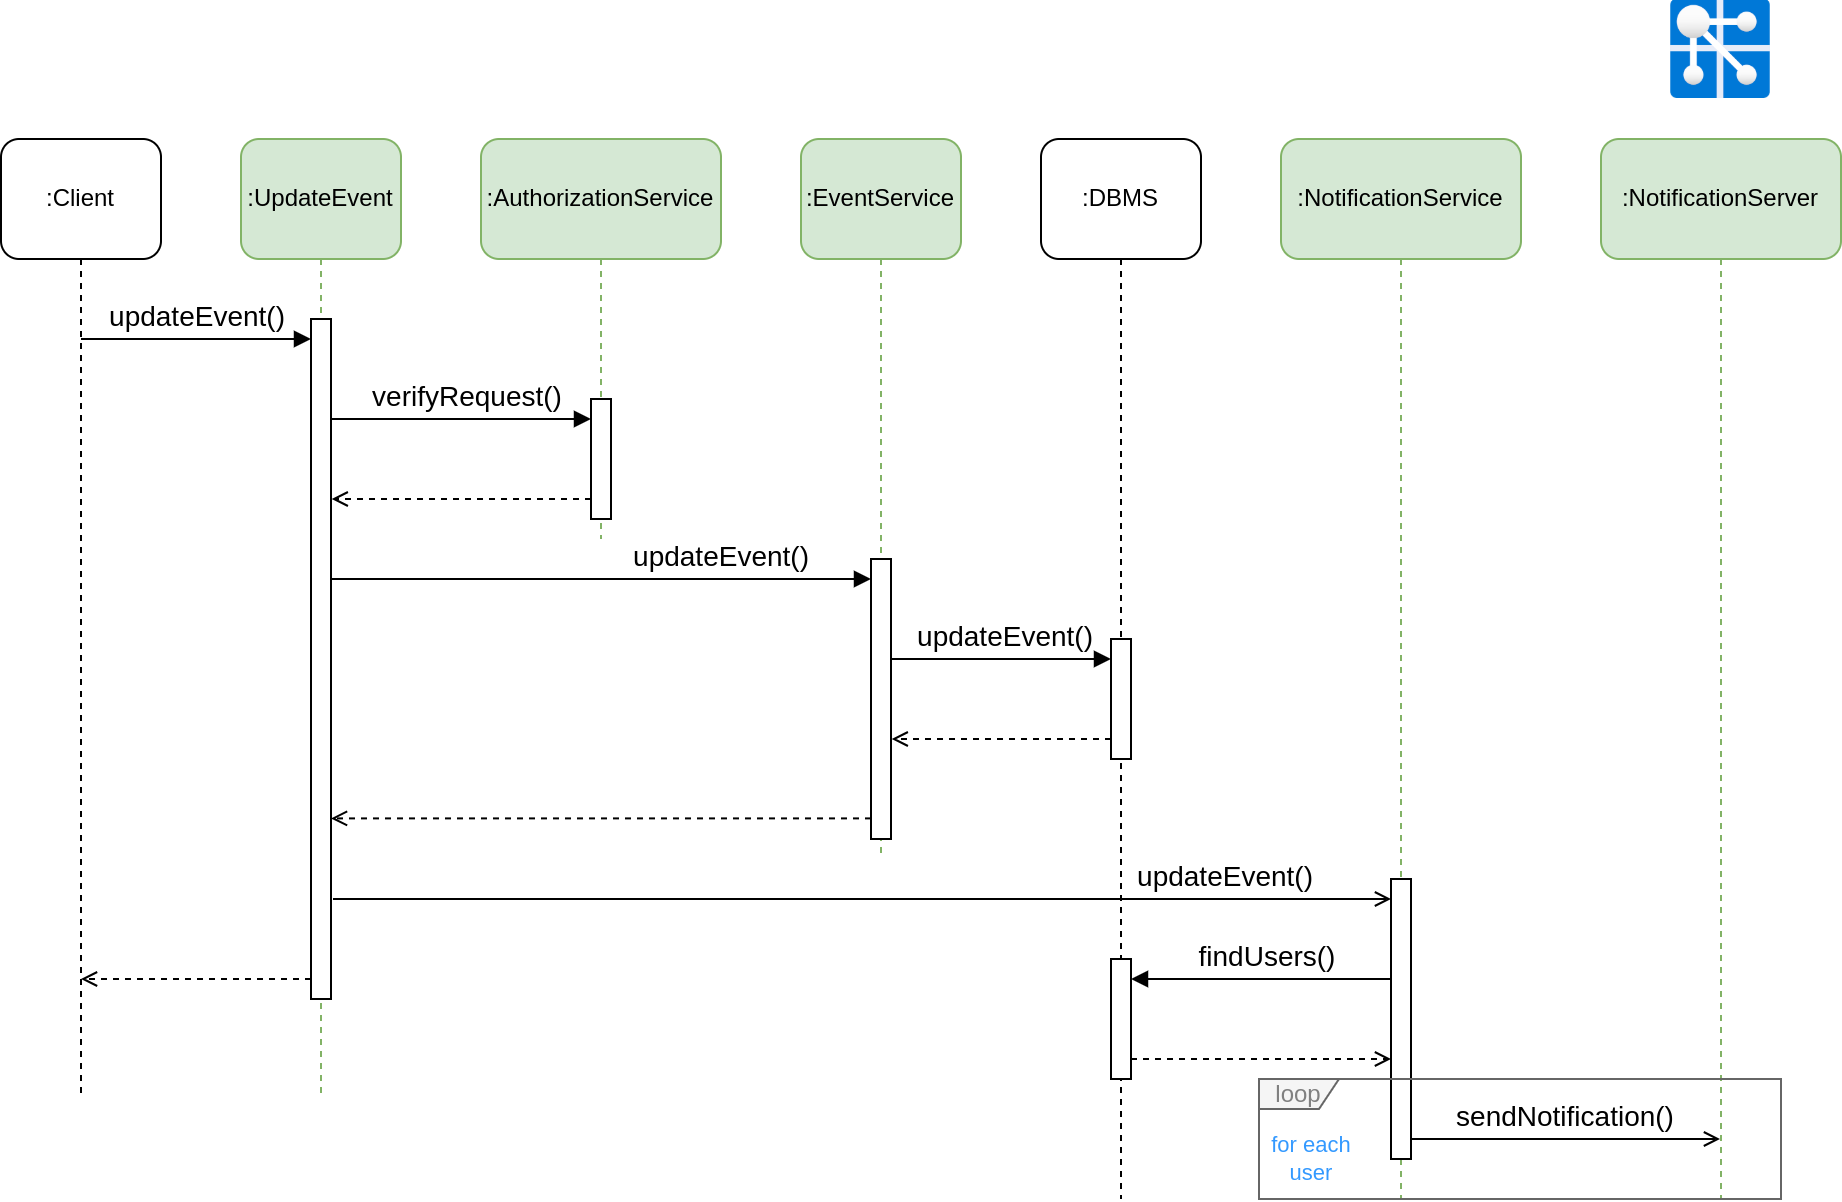
\includegraphics[width=\textwidth]{IIModificaEvento2.png}
    \caption{Interazione delle Azure Functions con AWPS}
\end{figure}	

La ricezione della notifica sul dispositivo dell’utente può comportare la richiesta al server dell’elemento modificato. La scelta di recuperare i dati tramite il server invece di includere i dati direttamente all’interno della notifica permette di uniformare il formato delle notifiche, semplificando la loro gestione e velocizzando l'invio; di diminuisce il volume dei dati trasmessi tramite WebSocket, garantendo la scalabilità delle notifiche; di migliorare la gestione degli errori da parte del server rendendoli più affidabili e di garantisce la possibilità di recuperare solo l’ultimo aggiornamento, riducendo il consumo totale dei dati.


\begin{figure}[h!]
    \centering
    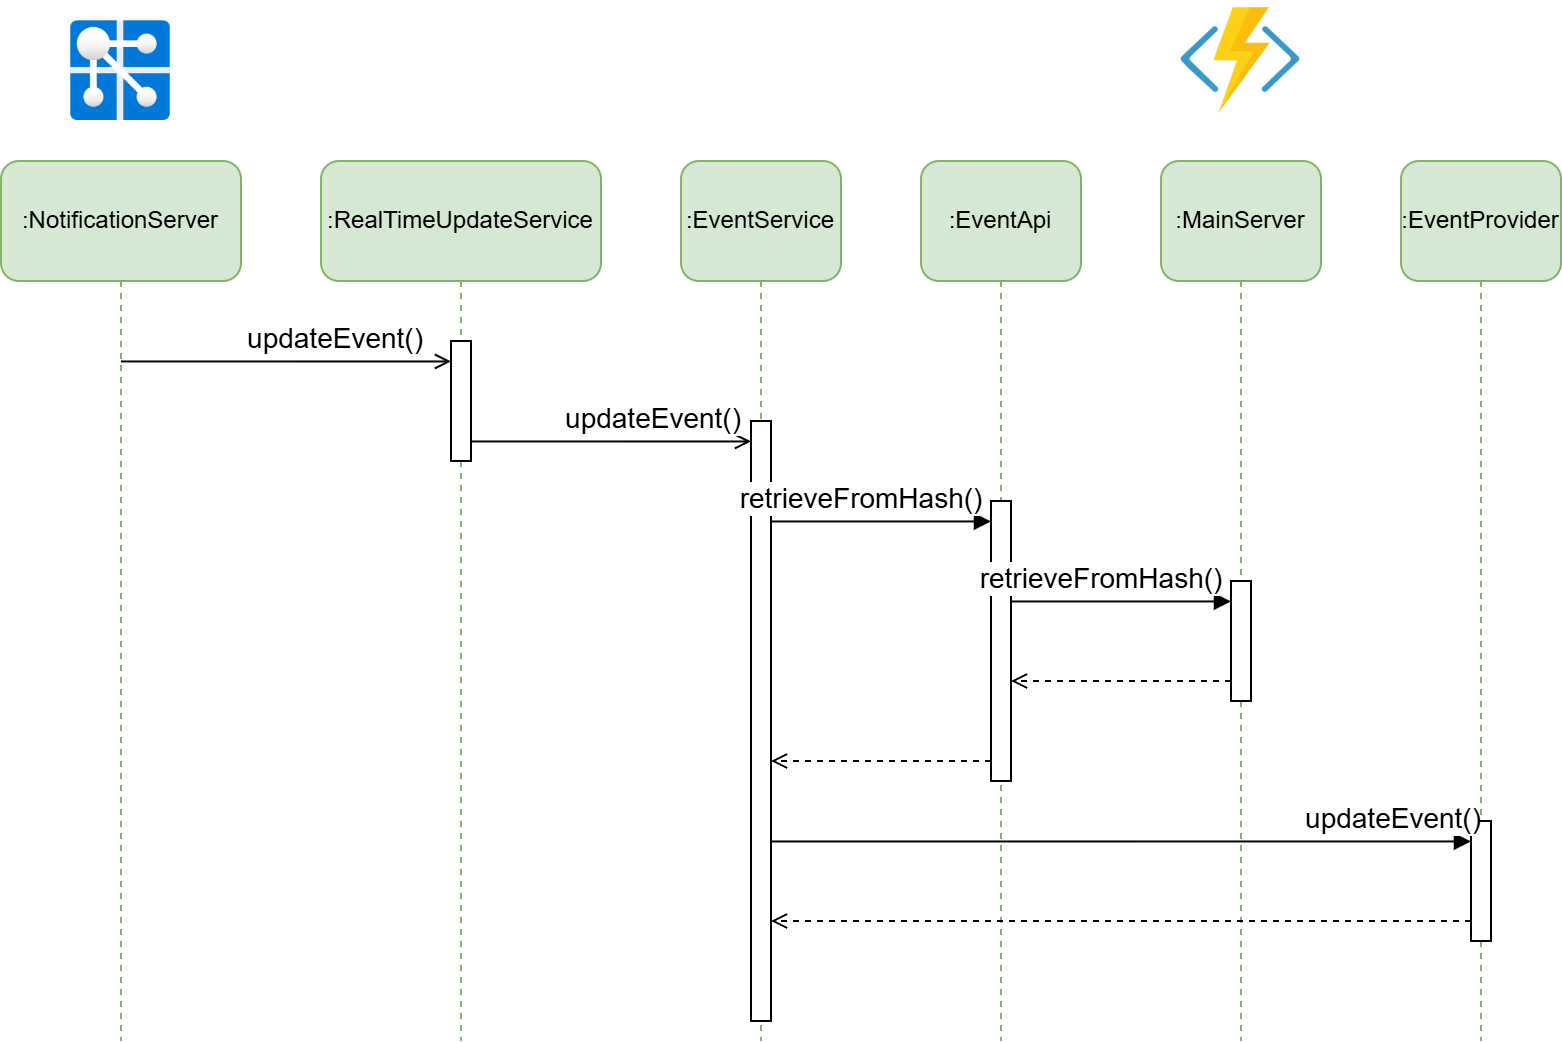
\includegraphics[width=\textwidth]{IIAggiornaEvento.png}
    \caption{Interazione tra AWPS e un client}
\end{figure}	

\clearpage
%\section{Gestione dei dati multimediali}

I file multimediali rappresentano un elemento centrale all’interno di un’applicazione orientata alla condivisione sociale,
contribuendo significativamente all’esperienza utente e all’interazione tra i partecipanti.
La possibilità di acquisire e condividere contenuti visivi, come immagini e video, consente di documentare eventi e attività,
favorendo una memoria collettiva e rafforzando il legame tra gli utenti.
In particolare, l’integrazione di materiale multimediale associato a eventi condivisi permette di preservare una rappresentazione più completa e dettagliata dell’esperienza vissuta,
migliorando l’engagement e la partecipazione all’interno della piattaforma, rappresentando uno dei punti di forza dell’applicazione.\\
\\
Tuttavia, la gestione dei file multimediali introduce complessità operative sia per gli utenti sia per il sistema stesso.
Da un lato, la selezione e l’invio dei contenuti possono rappresentare un onere significativo per l’utente, aumentando l’attrito nell’utilizzo dell’applicazione.
Per ottimizzare il processo e migliorare l’usabilità, è essenziale semplificare al massimo l’interazione richiesta,
automatizzando il recupero dei dati e limitando il ruolo dell’utente alla semplice conferma dei contenuti selezionati.
Questo approccio non solo semplifica l’esperienza d’uso, ma la rende più intuitiva e fruibile,
contribuendo anche a un incremento del tasso di adozione e della frequenza di utilizzo dell’applicazione.\\
\\
Parallelamente, la memorizzazione e il trasferimento di file multimediali pongono sfide significative a livello infrastrutturale,
in quanto tali dati presentano un impatto rilevante sulle risorse computazionali e sulla gestione dello storage.
Il volume elevato di richieste di caricamento e accesso ai file può infatti compromettere le prestazioni del sistema,
introducendo ritardi causati dal traffico di azioni che potrebbero influire negativamente sulle altre operazioni dell’applicazione.
Per garantire un’archiviazione efficiente e scalabile, è quindi necessario implementare una strategia di gestione della memoria
che separi il salvataggio dei file multimediali dal database principale, evitando di sovraccaricare il server applicativo.
Questa soluzione deve inoltre garantire un aggiornamento tempestivo delle informazioni, assicurando la sincronizzazione tra i dati archiviati e le modifiche effettuate dagli utenti.\\
\\
Per affrontare tali problematiche, un primo esame osserverà le modalità di recupero dei file multimediali,
con un focus sulle tecniche di selezione e rilevamento automatico delle immagini, nonché sui vincoli normativi e di sicurezza che ne regolano l’utilizzo.
In un secondo tempo l’analisi si concentrerà invece sulle strategie di salvataggio e gestione dello storage,
analizzando le diverse tipologie di archiviazione disponibili e le soluzioni implementate per garantire scalabilità, efficienza e riduzione dell’impatto sulle prestazioni del sistema.


\clearpage


\subsection{Recupero}

L’aggiunta di immagini a un evento prevede una fase preliminare di recupero, che consente all’utente di selezionare i file multimediali da associare. 
Il sistema offre due modalità principali di acquisizione: la selezione manuale da parte dell’utente, che può scegliere le immagini direttamente dalla memoria del dispositivo, 
e in alternativa, disponibile sui dispositivi mobili, un meccanismo automatizzato, che identifica le foto scattate durante lo svolgimento dell’evento.\\
\\
L’implementazione di questa funzionalità automatica di analisi della galleria per individuare i file multimediali desiderati  richiede l’accesso alla galleria fotografica del dispositivo, 
un’operazione subordinata al consenso esplicito dell’utente. 
Al primo avvio dell’applicazione perciò, il sistema richiede l’autorizzazione per accedere ai file multimediali, unitamente al permesso per la gestione delle notifiche. 
Nel caso in cui l’utente neghi l’accesso, la richiesta verrà riproposta ogni qualvolta il sistema rilevi la necessità di accedere alla galleria per il recupero delle immagini.\\
\\
Al termine di ogni evento, non appena possibile, l’applicazione avvia automaticamente un’analisi della galleria locale, individuando le immagini scattate durante tutta la durata dell’evento. 
Se il sistema rileva la presenza di contenuti pertinenti, ne memorizza temporaneamente i riferimenti in una memoria locale per poi inviare una notifica all’utente, 
informandolo del ritrovamento delle immagini. A questo punto, l’utente ha la possibilità di esaminare le immagini suggerite, escluderne alcune o confermarne l’intero set per il caricamento.\\
\clearpage
\begin{figure}[htb]
    \centering
    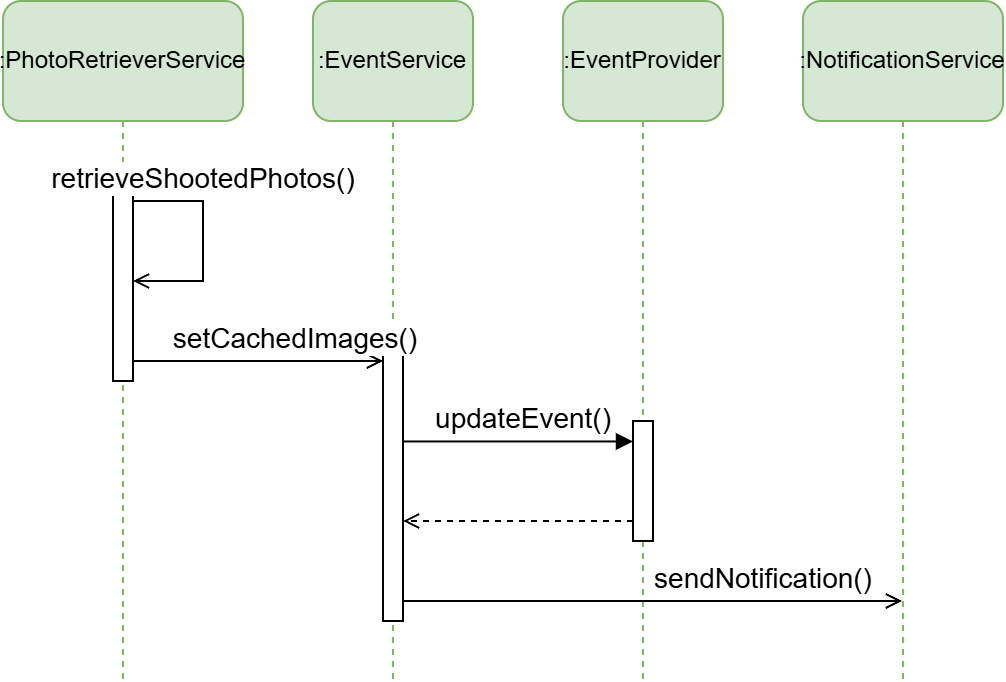
\includegraphics[height=0.45\textheight]{IIRecuperaImmagini.png}
    \caption{Interazione tra i componenti per il recupero delle immagini}
\end{figure}

Questa fase di conferma, oltre a garantire la trasparenza del servizio nei confronti dell’utente, 
riducendo il rischio di errori o caricamenti indesiderati, presenta anche vantaggi in termini di ottimizzazione delle prestazioni. 
\clearpage
Da un punto di vista normativo, la procedura di recupero e selezione automatica delle immagini è esplicitamente descritta nelle condizioni d’uso dell’applicazione, 
alle quali l’utente deve aderire con accettazione espressa prima di utilizzare il servizio. 
Tuttavia, la fase di conferma dell’utente non rappresenta un obbligo giuridico, 
poiché la responsabilità della pubblicazione di contenuti multimediali ricade sul soggetto che realizza la fotografia. 
In conformità con la normativa vigente in materia di tutela dell’immagine (art. 10 c.c. e artt. 96-97 della Legge n. 633/1941) e protezione dei dati personali (Regolamento UE 2016/679 – GDPR), 
chi scatta una fotografia è tenuto a ottenere il consenso delle persone ritratte prima di procedere alla sua pubblicazione.\\
\\
Come già affrontato nel capitolo precedente, le operazioni che coinvolgono la modifica di uno stesso componente del sistema 
sono soggette a vincoli di concorrenza per l’accesso alla risorsa di interesse. 
La conclusione di un evento condiviso tra più utenti potrebbe generare richieste simultanee per l’aggiunta di immagini associate a un medesimo evento. 
L’introduzione della fase di selezione introduce un ritardo nella fase di caricamento, 
dilatando la distribuzione temporale delle richieste e riducendo la probabilità di collisioni dovute a operazioni concorrenti sullo stesso elemento.
L’attesa della conferma dell’utente prevede infatti un ritardo fisiologico tra la fine dell’evento e l’effettivo caricamento delle immagini, 
contribuendo a distribuire le richieste nel tempo e limitando il rischio di congestione del server dovuta a operazioni simultanee su un singolo evento.\\
\\
Una volta completata la selezione da parte dell’utente, le immagini vengono inviate al server, che provvede al loro salvataggio e all’associazione con l’evento corrispondente.


\clearpage

\subsection{Salvataggio}

A differenza dei dati tradizionalmente scambiati all’interno del sistema, i file multimediali presentano dimensioni significativamente superiori, 
con diversità che si manifestano su ordini di grandezza rilevanti. 
Un salvataggio di tali file nel flusso di dati standard, allineandoli agli elementi logici, 
comporterebbe un rallentamento generale delle operazioni e un impatto significativo sulle prestazioni complessive del sistema. 
Per questo motivo, è necessaria una gestione della memoria specificamente progettata per l’archiviazione e il recupero di contenuti multimediali.	\\
\\
Inoltre, Le dimensioni delle immagini e dei video influenzano direttamente il tempo di elaborazione e il volume delle richieste, 
aumentando il carico computazionale su tutti i componenti del sistema. 
In aggiunta, la possibilità di allegare più file a un singolo evento implica che i tempi di caricamento più elevati dei file multimediali 
possano prolungare sensibilmente la durata delle transazioni necessarie per la modifica degli eventi, incidendo sulla reattività del sistema.\\
\\
\clearpage
\subsubsection{Persistenza}

La visualizzazione dei file multimediali riveste un'importanza secondaria rispetto ad altre funzionalità offerte dall'applicazione. 
Di conseguenza, è possibile accettare un maggiore tempo di caricamento, a condizione che ciò contribuisca a ridurre la latenza delle operazioni invece più rilevanti. 
Il salvataggio dei file multimediali direttamente nel database centrale comporterebbe un aumento significativo del volume delle richieste, 
determinando un maggiore impiego di risorse computazionali e un incremento dei tempi di caricamento. 
Questo fenomeno potrebbe incidere negativamente sulle prestazioni complessive del sistema, penalizzando l’esecuzione simultanea di altre operazioni.\\
\\
Per ottimizzare la gestione dei file multimediali, si adotta una distinzione della relazione tra l’oggetto logico e l'evento dai dati binari che lo compongono. 
In questo modo, la relazione tra il file e l’evento associato viene mantenuta indipendentemente dai dati binari che lo compongono. 
Una volta recuperati i riferimenti ai file multimediali associati all’evento in questione, sarà possibile ottenere poi i loro contenuti binari in un secondo momento, solo quando necessario.
Il modello del dominio illustrato in precedenza evidenzia la relazione logica tra gli eventi e i file associati (Photo).\\
\\
Considerando la necessità e la possibilità di archiviare i file multimediali su risorse differenti dal database centrale, 
è fondamentale individuare la soluzione più adatta alla loro persistenza. 
I principali servizi cloud per l’archiviazione di file multimediali si suddividono in tre categorie: Object Storage, File Storage e Block Storage.
Gli Object Storage gestiscono i file in un unico livello, con la possibilità di aggiungere metadati agli oggetti. 
A ciascun elemento viene associato un identificativo univoco che ne consente il recupero. 
L’accesso ai dati avviene tipicamente tramite API RESTful, che oltre ad offrire la possibilità di gestire i permessi, garantisce l’utilizzo su ampia scala. 
La presenza di un unico livello di indirizzamento permette una scalabilità pressoché illimitata, e un costo variabile in base alla quantità di dati memorizzati.
I File Storage organizzano i file in una struttura gerarchica di cartelle e sottocartelle, semplificando la gestione dei file e il controllo degli accessi. 
Oltre a facilitare un controllo ulteriore agli utenti, questa soluzione è compatibile con protocolli di accesso particolari. 
Tuttavia, la sua capacità e scalabilità, così come il costo effettivo, sono legati alla struttura dei file e alla capacità prevista dal piano selezionato.
Infine, i Block Storage gestiscono la memoria tramite la suddivisione dei dati in blocchi logici, salvati separatamente e ognuno dotato di identificativo univoco. 
Questa tecnologia offre elevate prestazioni per il recupero e la modifica dei dati, ma i costi aumentano all'incremento della quantità di dati presenti. 
La scalabilità è quindi limitata alla capacità assegnata al volume. Oltretutto, i costi sono elevati, particolarmente riguardo moli di grandi entità.\\
\\
Tra queste soluzioni, la categoria degli Object Storage risulta la più adatta alle esigenze del progetto di salvataggio dei file multimediali. 
La sua scalabilità illimitata consente di gestire grandi volumi di elementi con una ridotta interdipendenza tra loro. 
Inoltre, l’identificazione univoca di ciascun oggetto garantisce una rapida individuazione dei dati e un’efficiente risposta prestazionale a numerose richieste contemporanee.\\
\\
Nel contesto di Azure, il servizio di Object Storage fornito è rappresentato da Azure Blob Storage (ABS). 
ABS adotta un’organizzazione centrata su Container, entità logiche che raggruppano più file multimediali e introducono un livello di indirizzamento aggiuntivo. 
L’accesso in lettura ai dati avviene tramite protocollo API RESTful, con autenticazione per l’aggiunta di nuovi elementi. 
Per ogni evento viene creato un Container dedicato, contenente le immagini corrispondenti.\\
\\
Terminata la selezione dei file multimediali, prima dell’invio al server, i dispositivi client eseguono la compressione delle immagini, 
riducendo il consumo di banda e il volume dei dati totali trasmessi. 
Questa strategia consente di diminuire il carico computazionale sul server, migliorando l’efficienza complessiva del sistema.\\
\\
Il server, una volta ricevuta la richiesta, esegue una verifica dei permessi di accesso necessari e procede con il caricamento delle immagini nel Container associato all’evento. 
Al termine dell’operazione, il database viene aggiornato con i riferimenti ai nuovi file multimediali, e gli utenti vengono notificati della modifica avvenuta.\\
\\
La visualizzazione di un evento con immagini allegate comporta la richiesta parallela da parte delle singole immagini del dispositivo client verso ABS. 
Le immagini vengono identificate univocamente attraverso la combinazione dell’hash dell’immagine con quello del Container associato all’evento.\\
\\

\begin{figure}[h!]
    \centering
    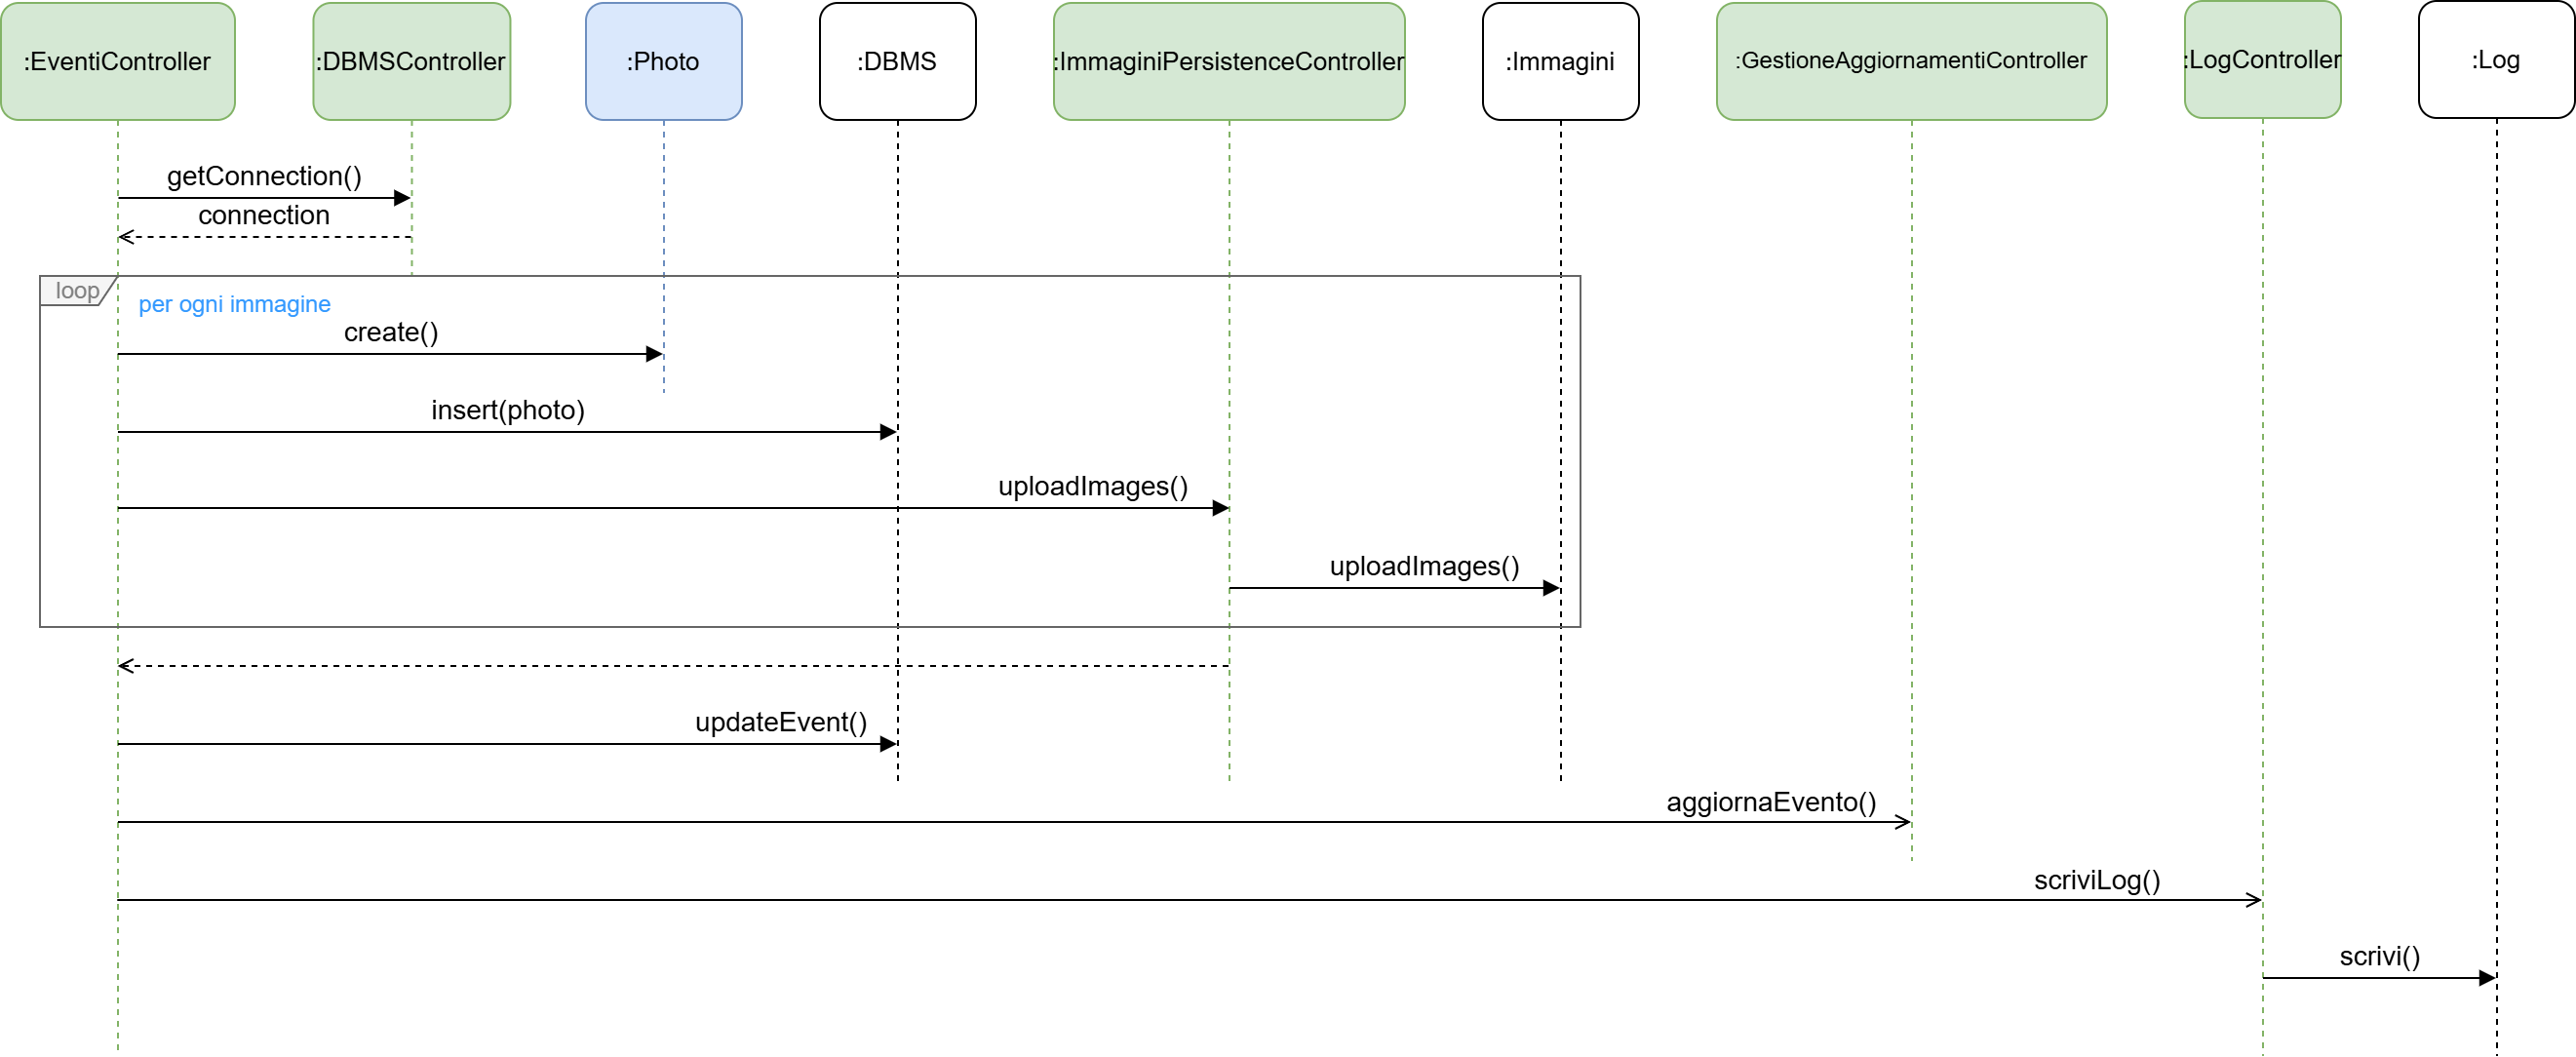
\includegraphics[width=\textwidth]{PIConfermaImmagini2.png}
    \caption{Interazione progettuale del server per il caricamento delle immagini }
\end{figure}

Tuttavia, l’accesso in lettura ai file multimediali in ABS risulta pubblico per impostazione predefinita, 
poiché la mancata definizione di ruoli comporta l’assenza di controlli espliciti sulle autorizzazioni delle richieste. 
Questo aspetto viene mitigato mediante l’uso di hash randomici sufficientemente lunghi, che riducono drasticamente la probabilità di collisione. 
Senza la conoscenza dell’hash corretto, un accesso non autorizzato alle immagini 
richiederebbe tentativi casuali estremamente numerosi nella speranza di trovare una combinazione corretta, rendendo un attacco altamente improbabile. 
Inoltre, anche in caso di compromissione di un hash, l’accesso sarebbe limitato a una singola immagine, senza fornire ulteriori informazioni sugli altri file memorizzati.

\clearpage

\subsubsection{Concorrenza }

Il caricamento delle immagini dalle Azure Functions al Container associato all’evento rappresenta un'operazione relativamente onerosa in termini di tempo, 
soprattutto se confrontata con le altre operazioni eseguite dal sistema. 
La gestione delle connessioni tra il server e il database relazionale richiede dunque scelte di dominio e sviluppo mirate a garantire un uso ottimale delle risorse, 
minimizzando il tempo di blocco e migliorando l'efficienza complessiva.\\
\\
Un elemento centrale nel processo di invio dati è la gestione dell’hash dell’elemento Photo, che deve corrispondere al file caricato. 
L’hash viene generato al momento della creazione dell’oggetto, ma il suo salvataggio nel database avviene solo dopo il completamento del caricamento del file multimediale. 
Questa strategia evita operazioni di scrittura e cancellazione superflue, ottimizzando le prestazioni del sistema. 
Ne consegue che il momento della creazione dell’oggetto Photo deve essere logicamente distinto dal suo effettivo salvataggio nel database.

Per realizzare un’astrazione ad alto livello della relazione con il database, Entity Framework Core (EF Core) fornisce una rappresentazione logica degli elementi, 
mantenendo un collegamento con le relative controparti fisiche. 
Grazie a questa caratteristica, è possibile creare un oggetto senza doverlo immediatamente memorizzare, consentendo un controllo più preciso e immediato sul flusso dei dati.\\
\\
La relazione uno a molti tra gli eventi e le immagini è implementata mappando fisicamente  sugli oggetti Photo, 
i quali contengono un riferimento all’identificativo dell’evento associato. 
Al momento del salvataggio, viene modificata esclusivamente la tabella relativa a Photo; 
tuttavia, tale operazione implica un blocco in scrittura anche sull’oggetto Event. 
Ciò avviene poiché l’oggetto Event è coinvolto a livello logico, come dimostrato anche dalla presenza di una lista virtuale contenente le immagini associate tra i suoi attributi.\\
\\
Per migliorare l’efficienza del caricamento, la trasmissione dei file multimediali verso il Container avviene in parallelo, 
riducendo il tempo complessivo necessario per completare l’operazione. 
Tuttavia, l’inserimento immediato di ciascun oggetto Photo nel database al termine di ogni caricamento comporterebbe un rischio di conflitti sull’oggetto Event 
e un potenziale sovraccarico del database. Per mitigare questi problemi, 
gli oggetti logici Photo delle trasmissioni avvenute con successo vengono temporaneamente conservati in memoria per essere salvati successivamente  in un’unica operazione.\\
\\
L'inserimento simultaneo di tutti gli elementi Photo validi all'interno di una stessa transazione consente di ottimizzare l’impatto sul database, 
riducendo i tempi di blocco sull’oggetto Event e minimizzando il rischio di collisioni tra richieste concorrenti. 
Questo approccio garantisce una maggiore scalabilità e una gestione più efficiente delle risorse del sistema coinvolte.\\
\\

\begin{figure}[h!]
    \centering
    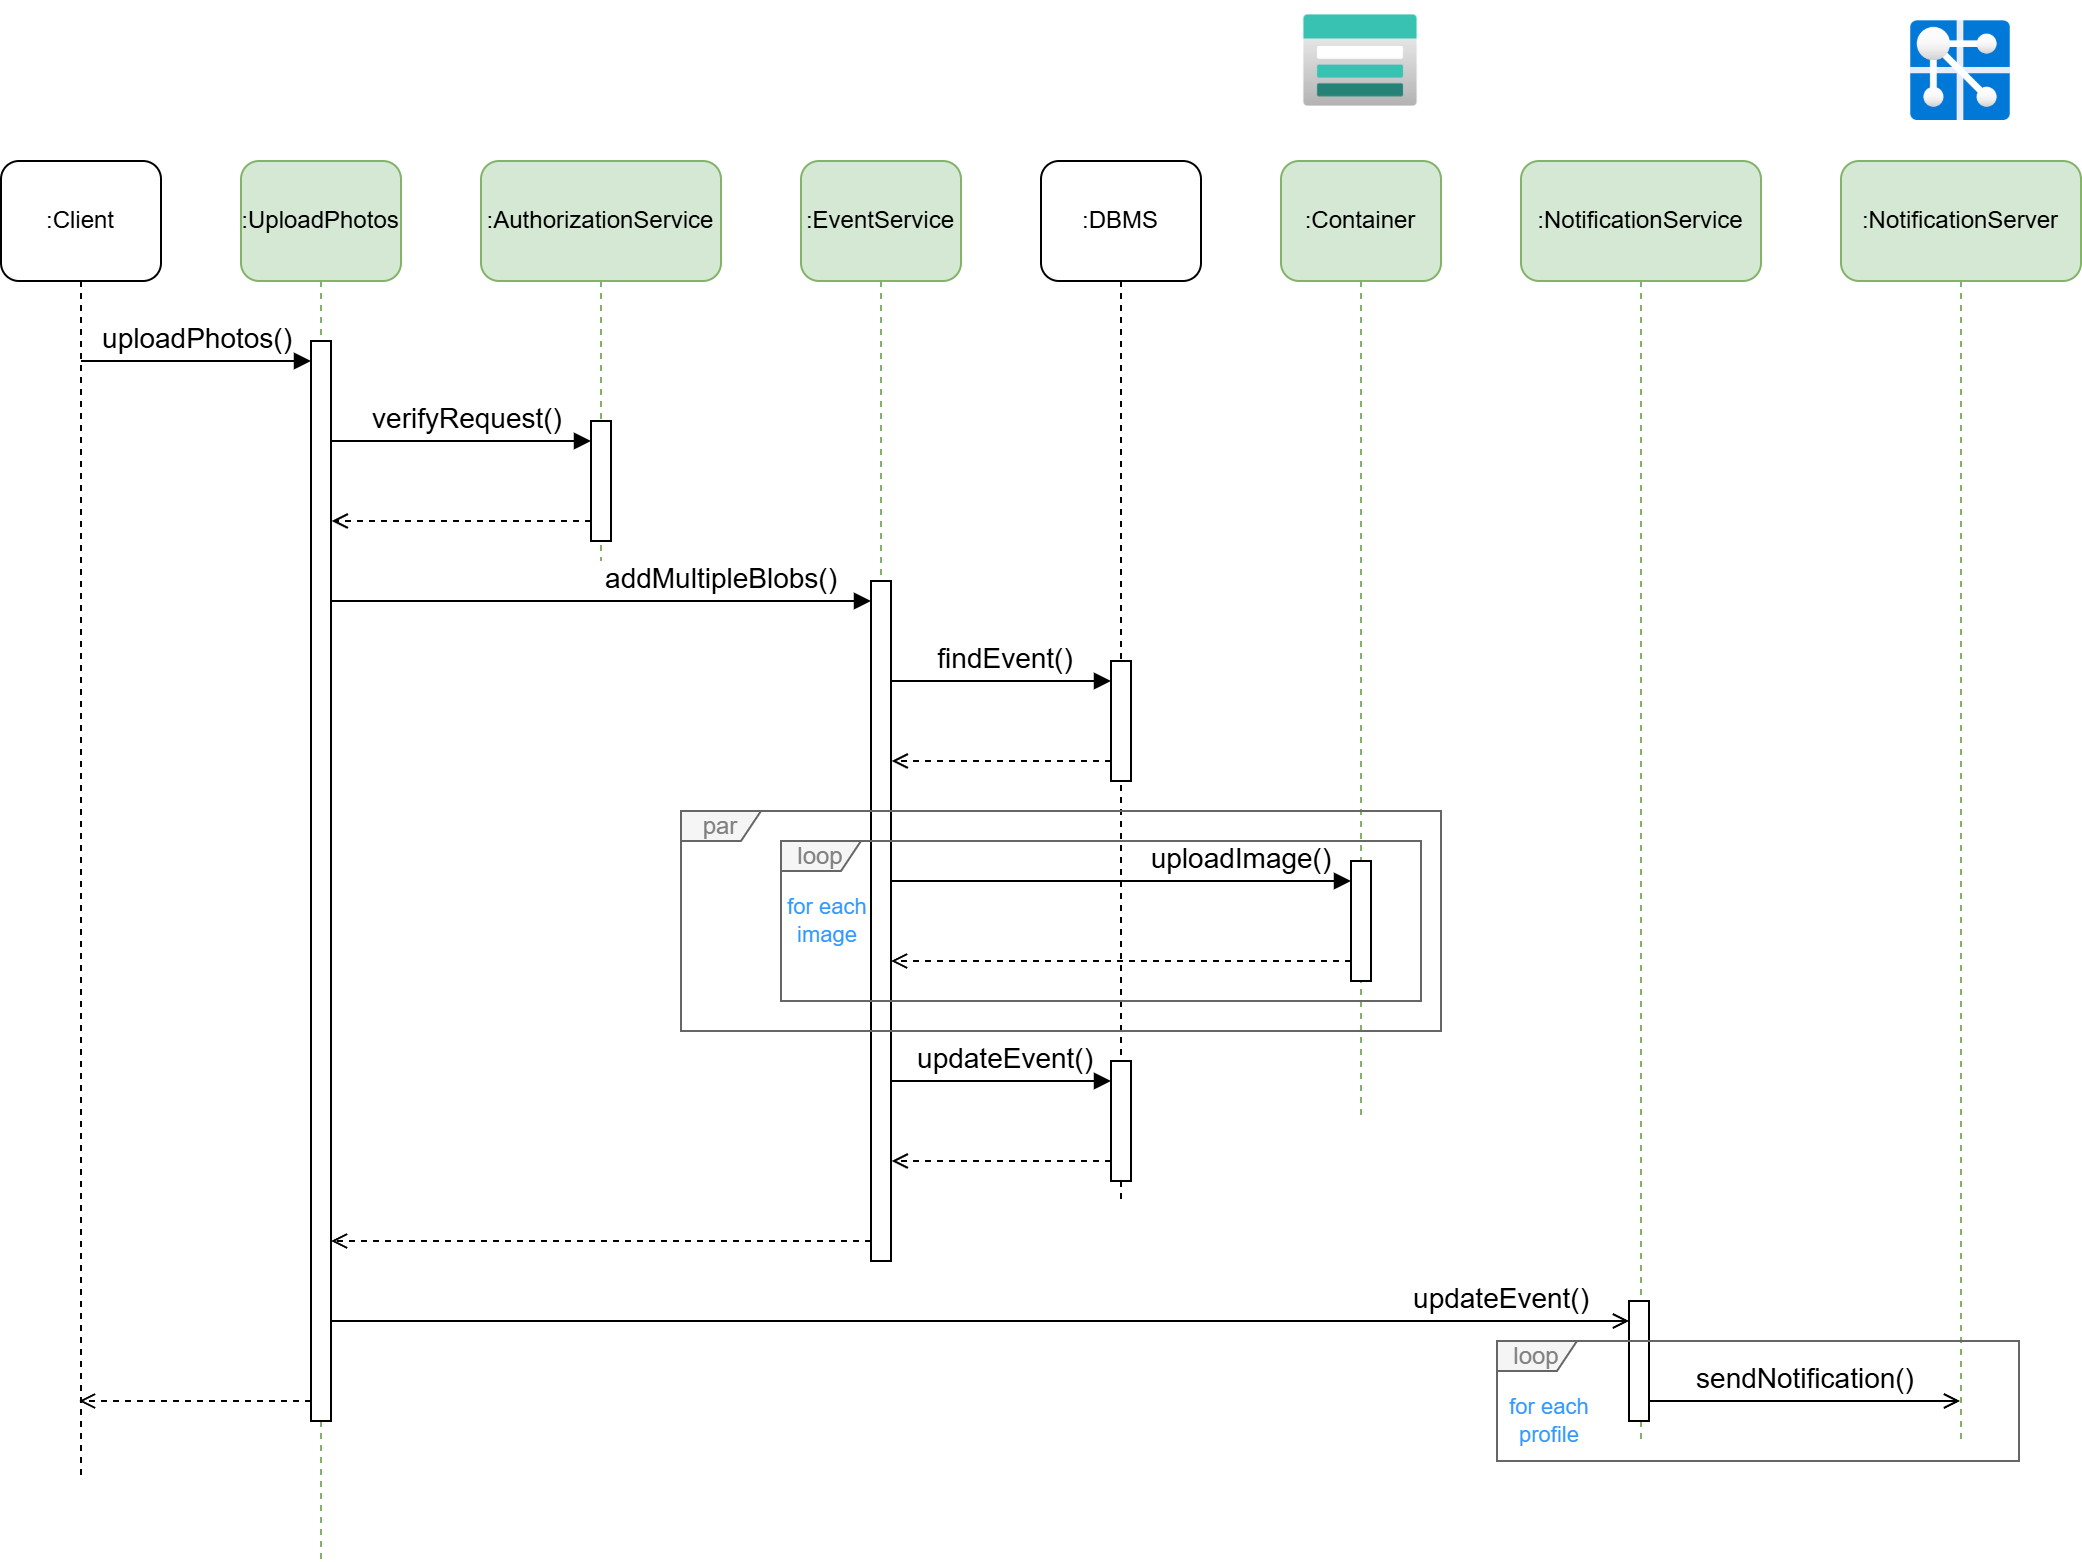
\includegraphics[width=\textwidth]{IICaricaImmagini.png}
    \caption{Interazione logica del server per il caricamento delle immagini }
\end{figure}

\clearpage
%
\chapter{Risultati}

\section{Velocità in lettura}

\begin{figure}[htbp]
    \begin{center}
        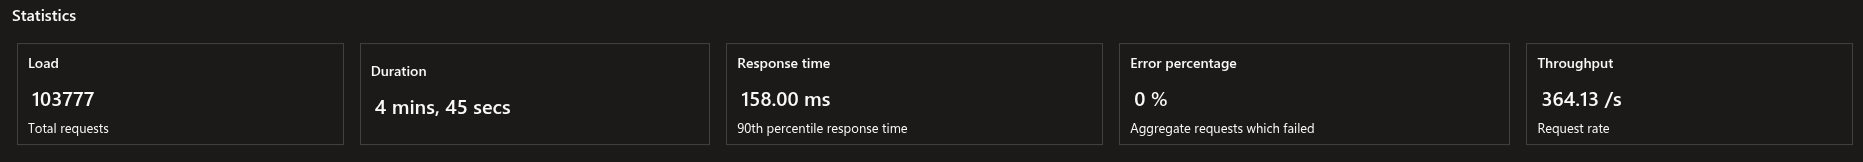
\includegraphics[width=\textwidth]{TestLettura1.png}
        \caption{158 ms su una media di 364 richieste al secondo}
    \end{center}
\end{figure}

\begin{figure}[htbp]
    \begin{center}
        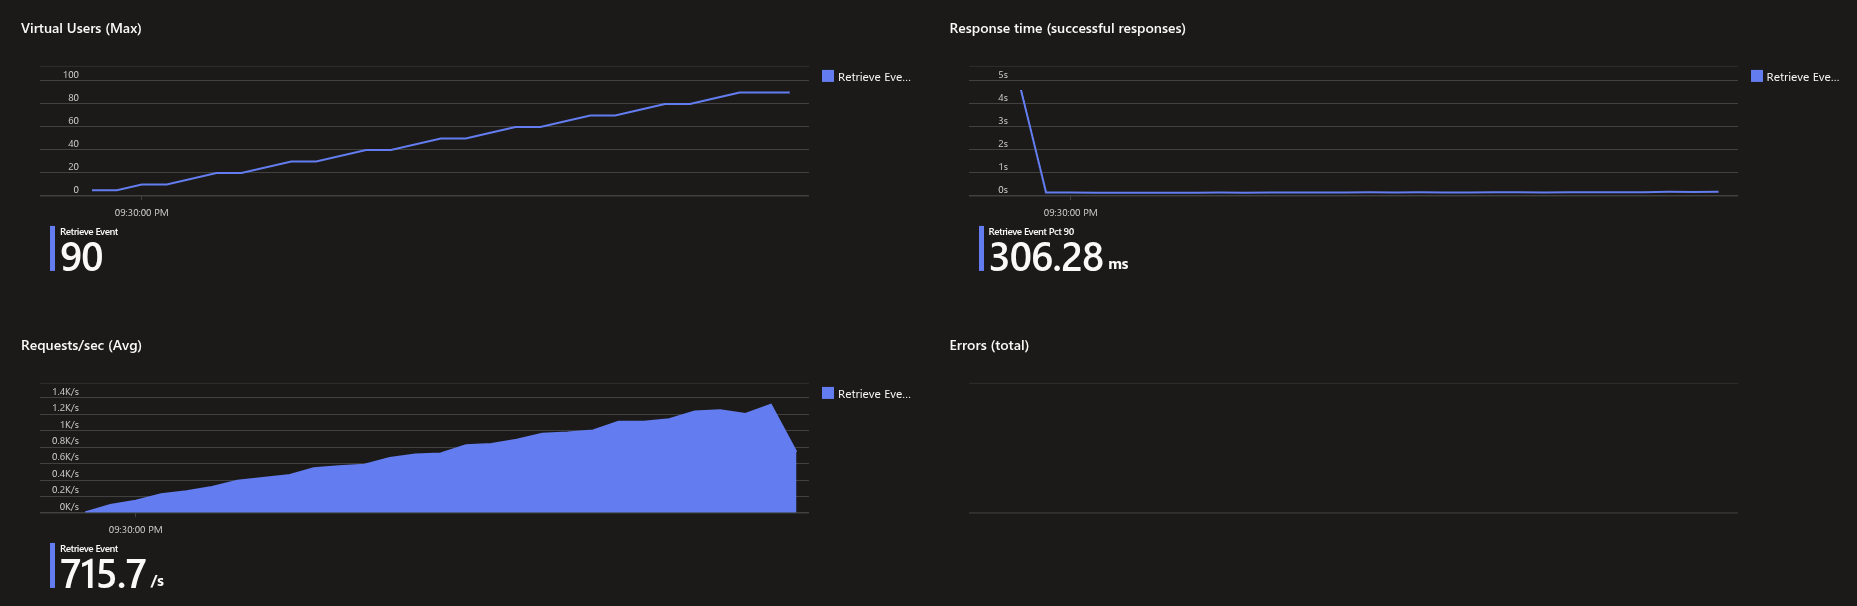
\includegraphics[width=\textwidth]{TestLettura2.png}
        \caption{il tempo di risposta non varia in base al numero di richieste}
    \end{center}
\end{figure}

\begin{figure}[htbp]
    \begin{center}
        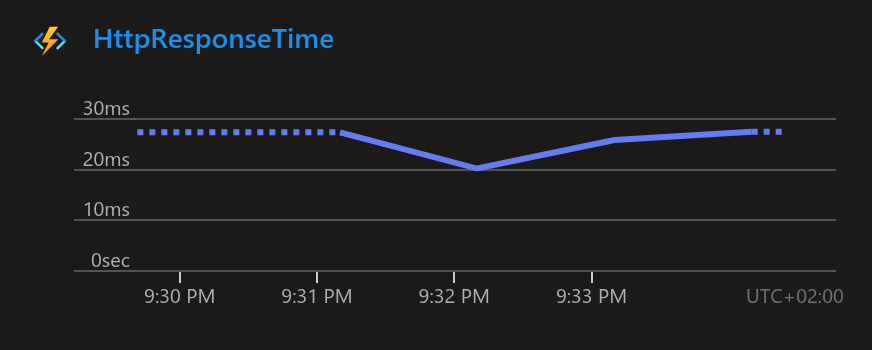
\includegraphics[width=\textwidth]{TestLettura3.png}
        \caption{Dettaglio della velocità senza tempo di trasmissione}
    \end{center}
\end{figure}
\clearpage
\section{Caricamento di immagini concorrenti}

\begin{figure}[htbp]
    \begin{center}
        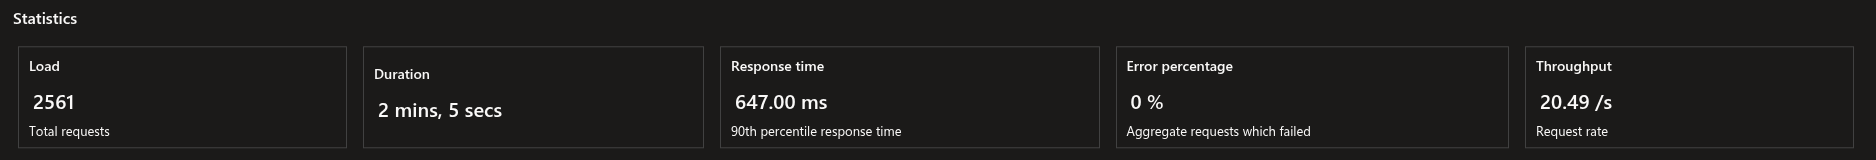
\includegraphics[width=\textwidth]{UploadImages1.png}
        \caption{2 MB di immagini in 600 ms 20 volte al secondo}  
    \end{center}
\end{figure}

\begin{figure}[htbp]
    \begin{center}
        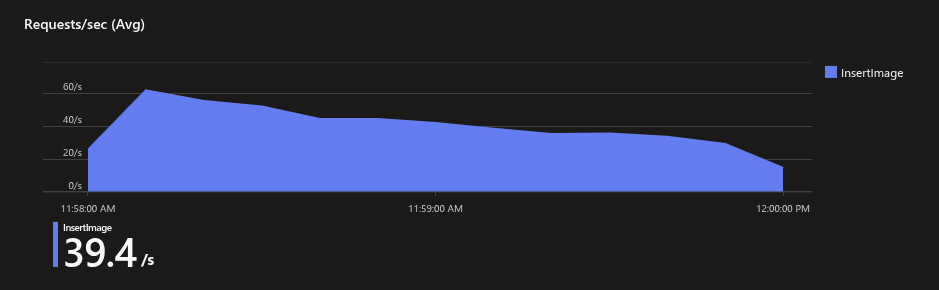
\includegraphics[width=\textwidth]{UploadImages3.png}
        \caption{Andamento delle richieste}  
    \end{center}
\end{figure}

\begin{figure}[htbp]
    \begin{center}
        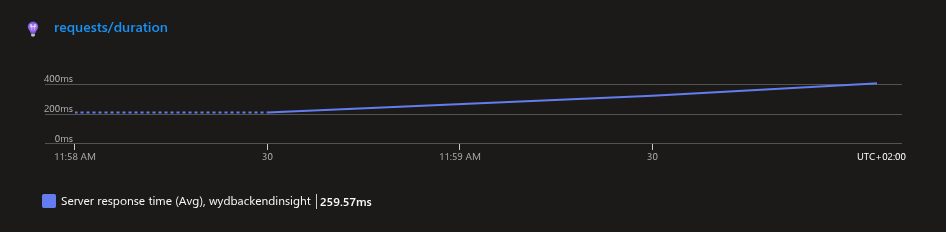
\includegraphics[width=\textwidth]{UploadImages2.png}
        \caption{Dettaglio della velocità richiesta dal server}
    \end{center}
\end{figure}


\clearpage
\chapter*{Conclusione}
\addcontentsline{toc}{chapter}{Conclusione}

\begin{figure}[htbp]
    \begin{center}
        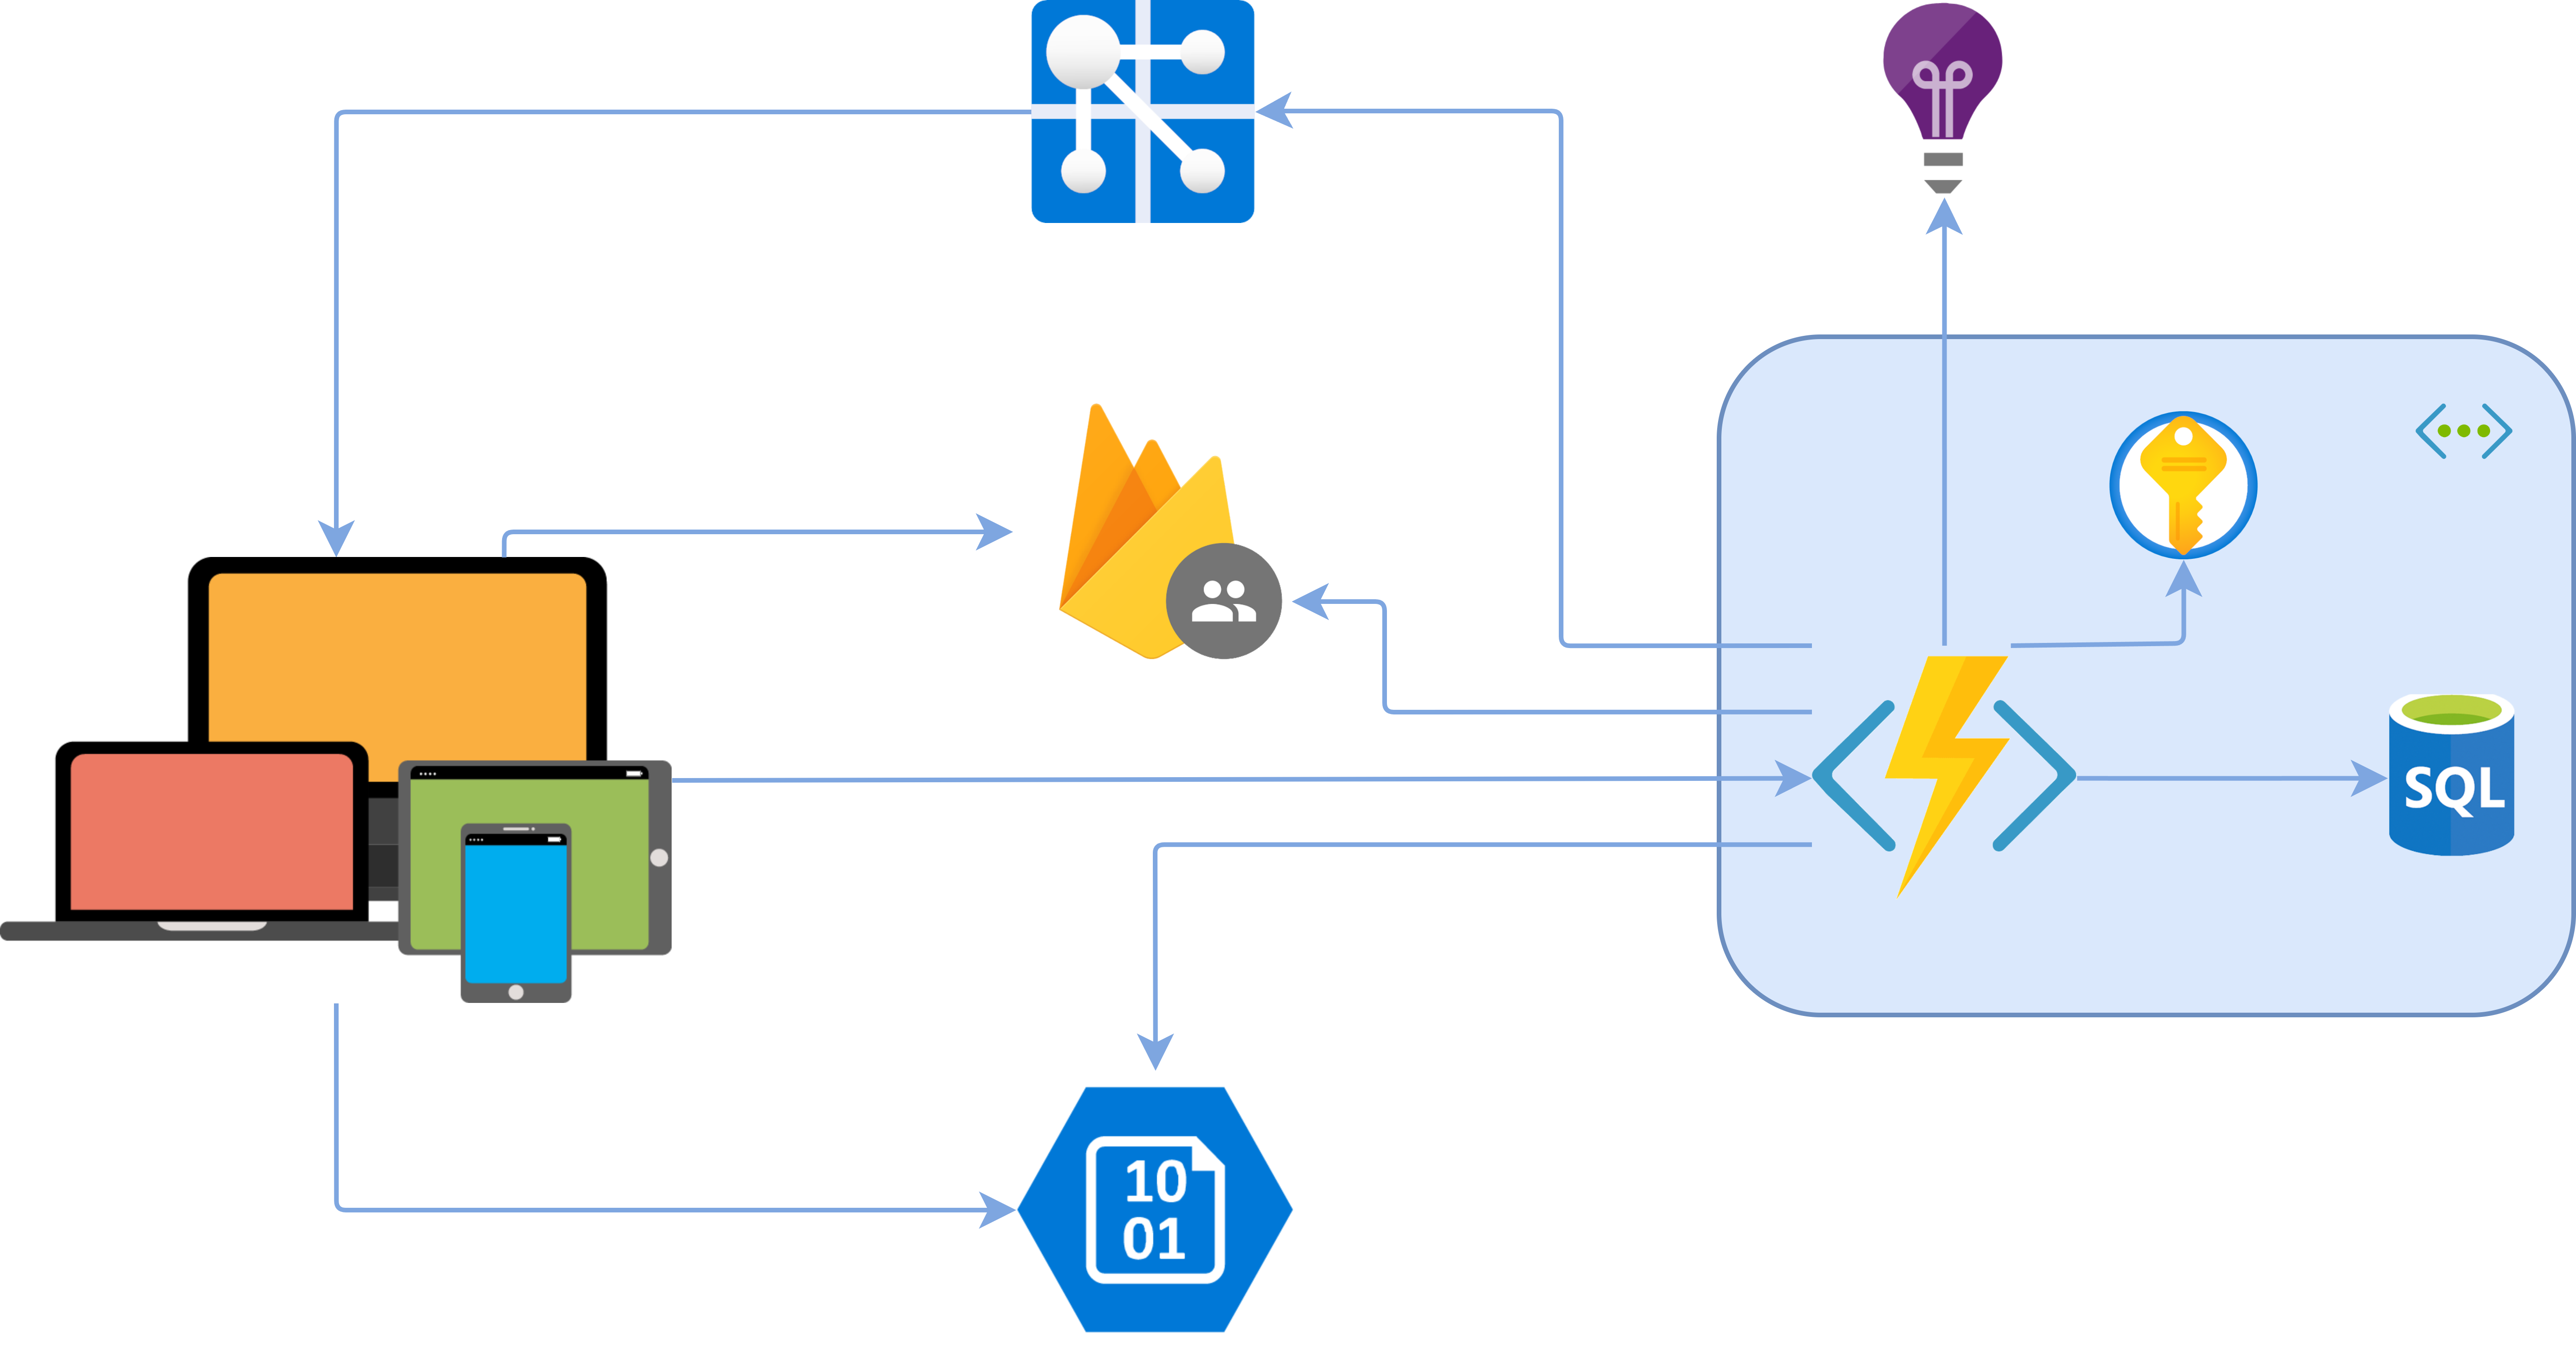
\includegraphics[width=\textwidth]{ImplementazioneArchitettura.png}
        \caption{Grafico dell'architettura finale}
    \end{center}
\end{figure}
\clearpage

\section{Sviluppi futuri}
Gli sviluppi futuri potranno comprendere, in base a decisioni di marketing:
\begin{itemize}
    \item La visualizzazione degli impegni degli altri profili
    \item L'implementazione di una chat per ogni gruppo
    \item Sviluppo di strumenti utili all'organizzazione dei gruppi, quali:
          \begin{itemize}
              \item form per combinare le disponibilità reciproche
              \item appunti condivisi(liste della spesa o note su chi porta cosa)
              \item calcolo delle spese compiute da ciascun componente
          \end{itemize}
    \item La creazione di profili pubblici che possono essere seguiti
    \item La creazione di eventi pubblici
    \item Una funzionalità di ricerca degli eventi o dei profili pubblici
    \item Supporto alla gestione di prenotazione e organizzazione degli eventi, dalle liste di attesa alla vendita dei biglietti
    \item La possibilità per le aziende di gestire in locale il proprio server e i relativi dati
\end{itemize}
\clearpage

\chapter*{Fonti bibliografiche e sitografia}
\addcontentsline{toc}{chapter}{Fonti bibliografiche e sitografia}

Object Management Group, OMG Unified Modelling Language Version 2.5.1, December 2017, https://www.omg.org/spec/UML/2.5.1/PDF

\end{document}